\documentclass[12pt]{extarticle}
\usepackage[paperwidth=15in,paperheight=7.2in]{geometry}
\usepackage{amsmath}
\usepackage{hyperref}
\usepackage{multirow}
\usepackage{pdfpages}
\usepackage[utf8]{inputenc}
\title{Kaon mixing: chiral and continuum extrapolations}
\author{R Mukherjee}
\date{\today}
\begin{document}
\maketitle
\tableofcontents
\clearpage
\begin{figure}
\centering
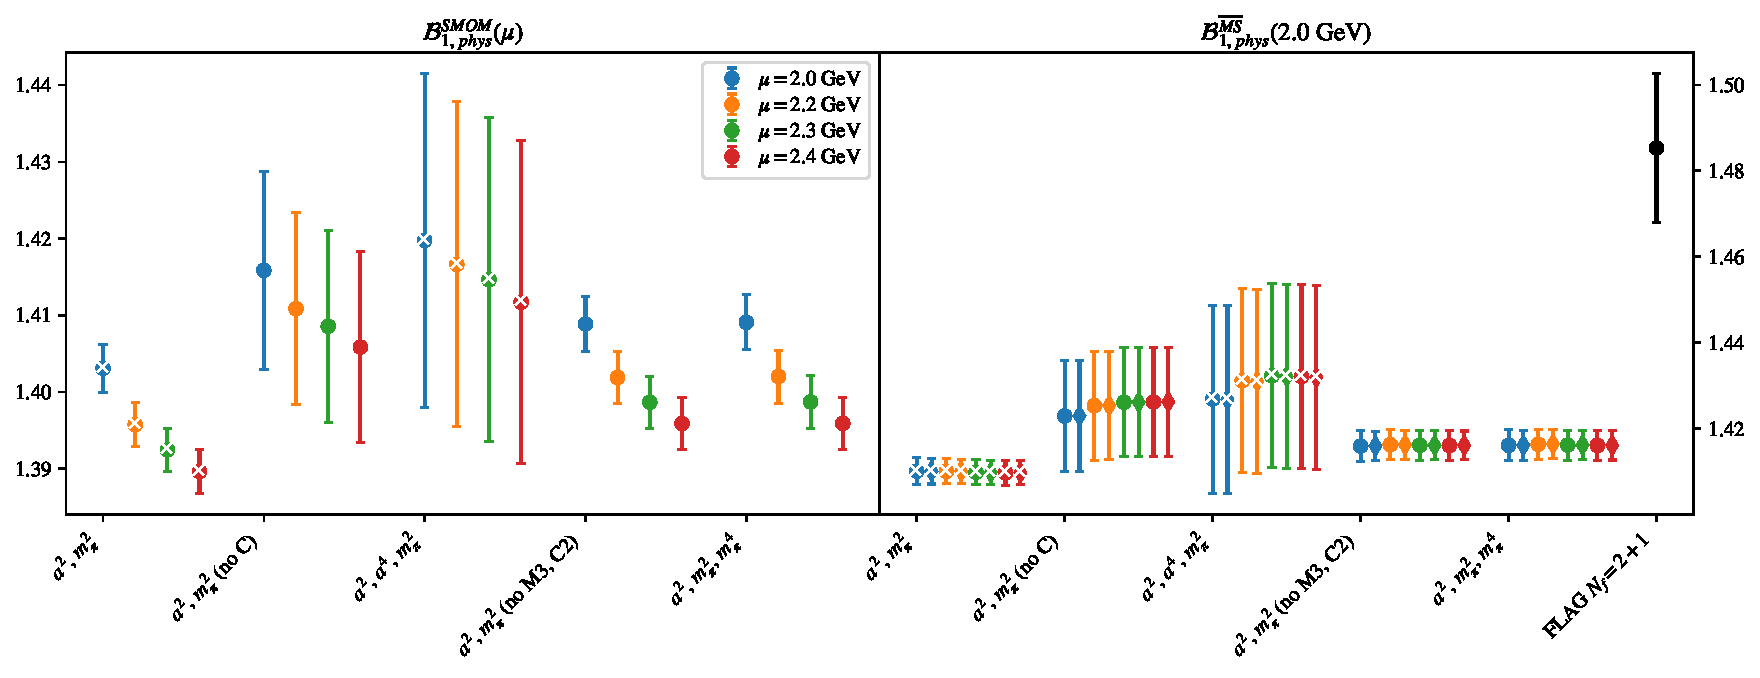
\includegraphics[page=1, width=1.1\textwidth]{VVpAA/SUSY/fit_summary_bag.pdf}
\caption{$\mathcal{B}_{1}$\\(left) $\mathcal{B}_{phys}$ in RI/SMOM scheme from fit variations (fits with $p$-value $<0.05$ marked with ``$\times$"). \\(right) $\mathcal{B}_{phys}$ in $\overline{MS}$ computed using $\mathcal{B}^{\overline{MS}} = R^{\overline{MS}\leftarrow SMOM}(2.0)\sigma_{npt}(2.0,\mu) \mathcal{B}^{SMOM}(\mu)$.}
\end{figure}
\clearpage
\begin{figure}
\centering
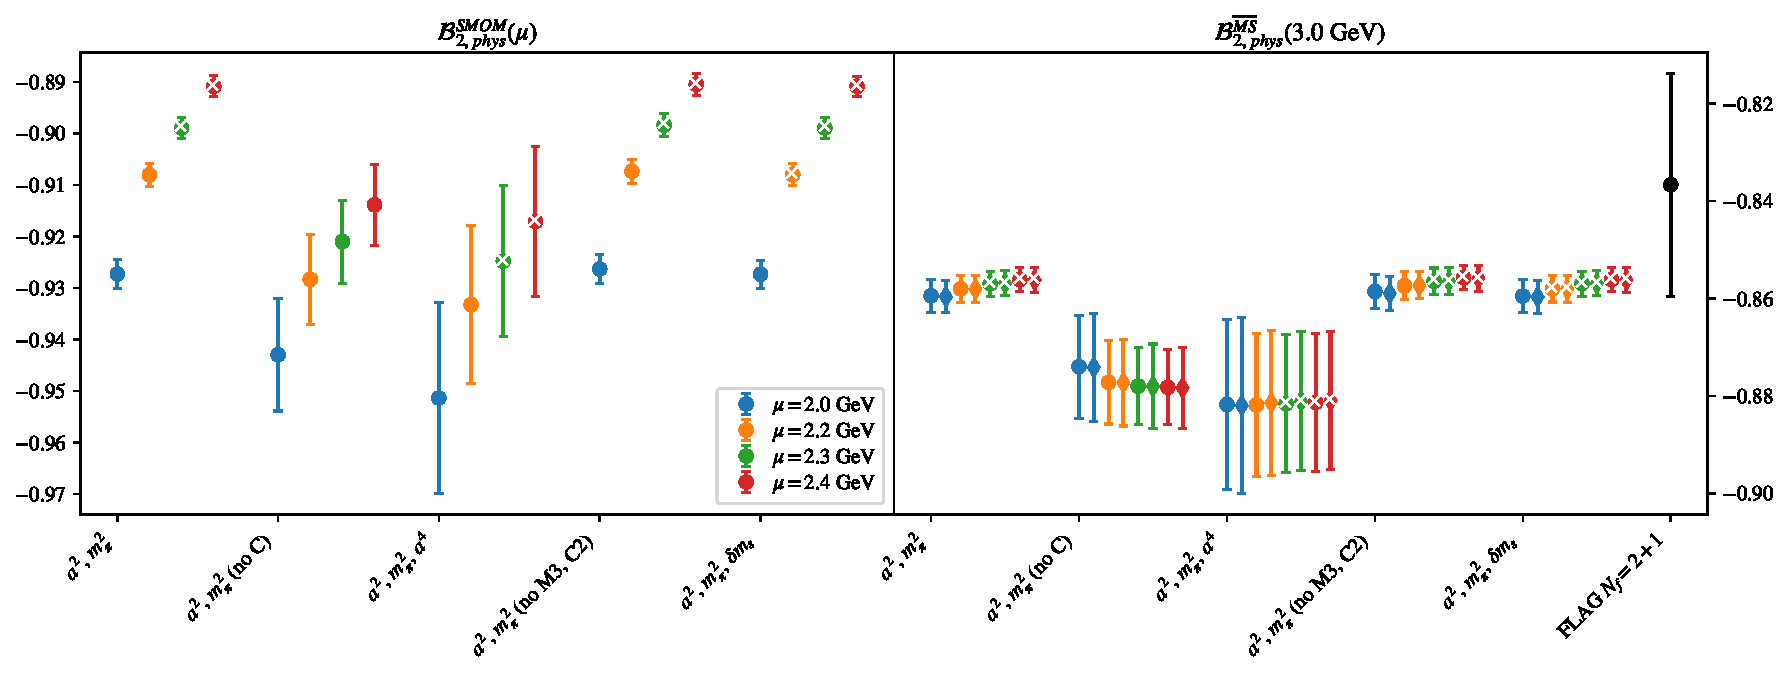
\includegraphics[page=1, width=1.1\textwidth]{VVmAA/SUSY/fit_summary_bag.pdf}
\caption{$\mathcal{B}_{2}$\\(left) $\mathcal{B}_{phys}$ in RI/SMOM scheme from fit variations (fits with $p$-value $<0.05$ marked with ``$\times$"). \\(right) $\mathcal{B}_{phys}$ in $\overline{MS}$ computed using $\mathcal{B}^{\overline{MS}} = R^{\overline{MS}\leftarrow SMOM}(3.0)\sigma_{npt}(3.0,\mu) \mathcal{B}^{SMOM}(\mu)$.}
\end{figure}
\clearpage
\begin{figure}
\centering
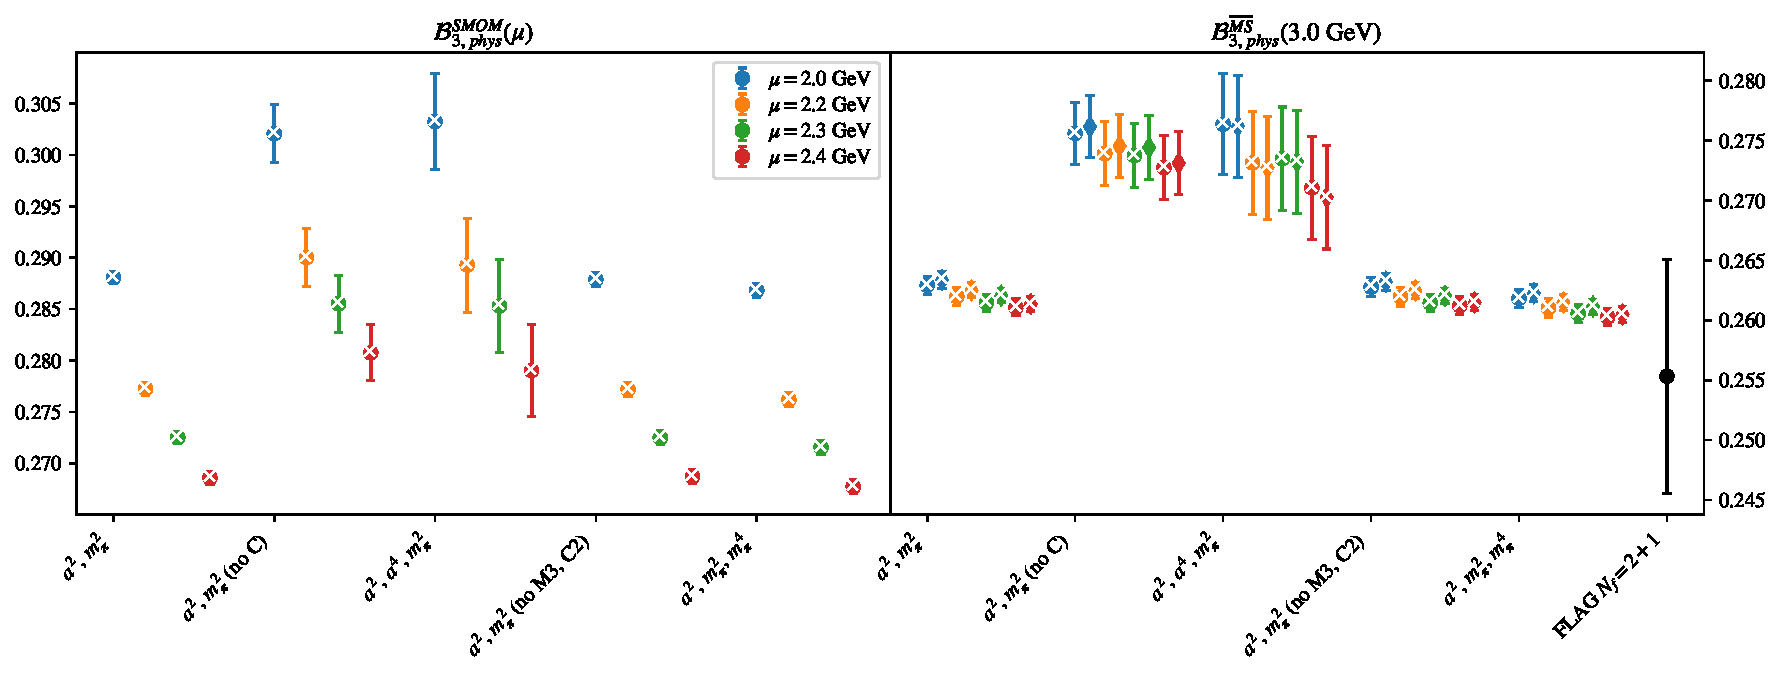
\includegraphics[page=1, width=1.1\textwidth]{SSmPP/SUSY/fit_summary_bag.pdf}
\caption{$\mathcal{B}_{3}$\\(left) $\mathcal{B}_{phys}$ in RI/SMOM scheme from fit variations (fits with $p$-value $<0.05$ marked with ``$\times$"). \\(right) $\mathcal{B}_{phys}$ in $\overline{MS}$ computed using $\mathcal{B}^{\overline{MS}} = R^{\overline{MS}\leftarrow SMOM}(3.0)\sigma_{npt}(3.0,\mu) \mathcal{B}^{SMOM}(\mu)$.}
\end{figure}
\clearpage
\begin{figure}
\centering
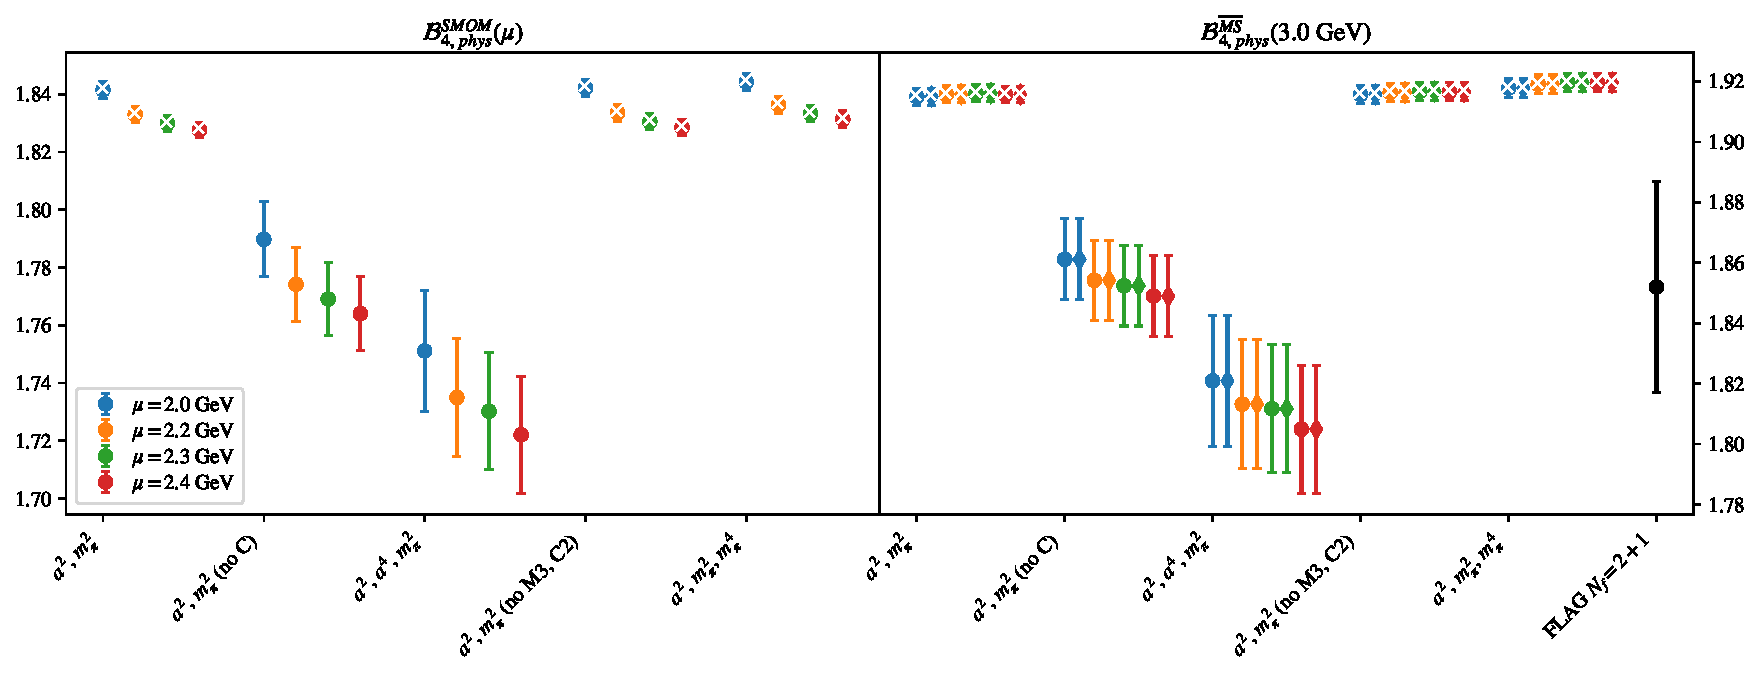
\includegraphics[page=1, width=1.1\textwidth]{SSpPP/SUSY/fit_summary_bag.pdf}
\caption{$\mathcal{B}_{4}$\\(left) $\mathcal{B}_{phys}$ in RI/SMOM scheme from fit variations (fits with $p$-value $<0.05$ marked with ``$\times$"). \\(right) $\mathcal{B}_{phys}$ in $\overline{MS}$ computed using $\mathcal{B}^{\overline{MS}} = R^{\overline{MS}\leftarrow SMOM}(3.0)\sigma_{npt}(3.0,\mu) \mathcal{B}^{SMOM}(\mu)$.}
\end{figure}
\clearpage
\begin{figure}
\centering
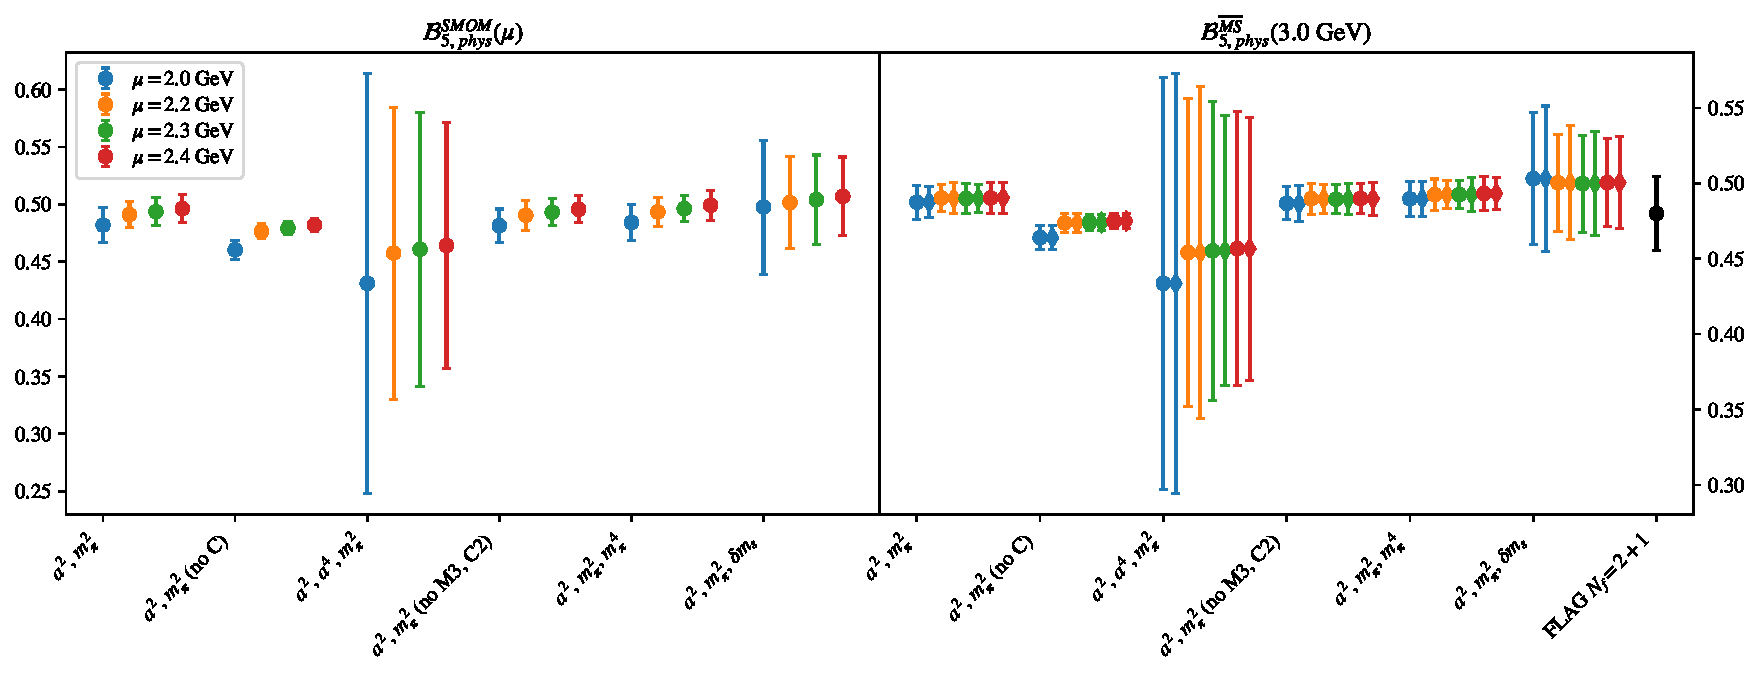
\includegraphics[page=1, width=1.1\textwidth]{TT/SUSY/fit_summary_bag.pdf}
\caption{$\mathcal{B}_{5}$\\(left) $\mathcal{B}_{phys}$ in RI/SMOM scheme from fit variations (fits with $p$-value $<0.05$ marked with ``$\times$"). \\(right) $\mathcal{B}_{phys}$ in $\overline{MS}$ computed using $\mathcal{B}^{\overline{MS}} = R^{\overline{MS}\leftarrow SMOM}(3.0)\sigma_{npt}(3.0,\mu) \mathcal{B}^{SMOM}(\mu)$.}
\end{figure}
\clearpage
\section{$\mathcal{B}_1$}
\begin{table}[h!]
\begin{center}
\begin{tabular}{|c|c|c|c|c|c|}
\hline
$\mu$ (GeV) & $a^2$, $m_\pi^2$& $a^2$, $m_\pi^2$ (no C)& $a^2$, $a^4$, $m_\pi^2$& $a^2$, $m_\pi^2$ (no M3, C2)& $a^2$, $m_\pi^2$, $m_\pi^4$\\
\hline
2.0& \hyperlink{VVpAA/SUSY/a2m2_20.pdf.1}{\textbf{1.4039(27)}: 1.85 (0.099)} & \hyperlink{VVpAA/SUSY/a2m2noC_20.pdf.1}{\textbf{1.416(12)}: 0.913 (0.401)} & \hyperlink{VVpAA/SUSY/a2a4m2_20.pdf.1}{\textbf{1.421(21)}: 2.14 (0.073)} & \hyperlink{VVpAA/SUSY/a2m2mcut_20.pdf.1}{\textbf{1.4090(32)}: 0.264 (0.852)} & \hyperlink{VVpAA/SUSY/a2m2m4_20.pdf.1}{\textbf{1.4093(33)}: 0.695 (0.595)}\\
2.2& \hyperlink{VVpAA/SUSY/a2m2_22.pdf.1}{\textbf{1.3964(27)}: 2.182 (0.053)} & \hyperlink{VVpAA/SUSY/a2m2noC_22.pdf.1}{\textbf{1.410(12)}: 1.153 (0.316)} & \hyperlink{VVpAA/SUSY/a2a4m2_22.pdf.1}{\textbf{1.417(21)}: 2.48 (0.042)} & \hyperlink{VVpAA/SUSY/a2m2mcut_22.pdf.1}{\textbf{1.4018(32)}: 0.36 (0.782)} & \hyperlink{VVpAA/SUSY/a2m2m4_22.pdf.1}{\textbf{1.4021(33)}: 0.916 (0.453)}\\
2.3& \hyperlink{VVpAA/SUSY/a2m2_23.pdf.1}{\textbf{1.3931(27)}: 2.268 (0.045)} & \hyperlink{VVpAA/SUSY/a2m2noC_23.pdf.1}{\textbf{1.408(12)}: 1.199 (0.302)} & \hyperlink{VVpAA/SUSY/a2a4m2_23.pdf.1}{\textbf{1.415(21)}: 2.556 (0.037)} & \hyperlink{VVpAA/SUSY/a2m2mcut_23.pdf.1}{\textbf{1.3986(32)}: 0.411 (0.745)} & \hyperlink{VVpAA/SUSY/a2m2m4_23.pdf.1}{\textbf{1.3988(33)}: 0.984 (0.415)}\\
2.4& \hyperlink{VVpAA/SUSY/a2m2_24.pdf.1}{\textbf{1.3902(26)}: 2.318 (0.041)} & \hyperlink{VVpAA/SUSY/a2m2noC_24.pdf.1}{\textbf{1.405(12)}: 1.224 (0.294)} & \hyperlink{VVpAA/SUSY/a2a4m2_24.pdf.1}{\textbf{1.412(21)}: 2.618 (0.033)} & \hyperlink{VVpAA/SUSY/a2m2mcut_24.pdf.1}{\textbf{1.3959(32)}: 0.412 (0.744)} & \hyperlink{VVpAA/SUSY/a2m2m4_24.pdf.1}{\textbf{1.3960(33)}: 1.0 (0.406)}\\
\hline
\end{tabular}
\caption{Physical point value from chiral and continuum extrapolation at renormalisation scale $\mu$. Entries are \textbf{value(error)}: $\chi^2/\text{DOF}$ ($p$-value).}
\end{center}
\end{table}
\begin{table}[h!]
\begin{center}
\begin{tabular}{|c c|c|c|c|c|c|}
\hline
$\mu$ (GeV) &  & $a^2$, $m_\pi^2$& $a^2$, $m_\pi^2$ (no C)& $a^2$, $a^4$, $m_\pi^2$& $a^2$, $m_\pi^2$ (no M3, C2)& $a^2$, $m_\pi^2$, $m_\pi^4$\\
\hline
\multirow{2}{0.5in}{2.0} & $\alpha$ & 0.0935(71)& 0.047(52)& -0.022& 0.0813(83)& 0.0811(83)\\
 & $\beta$ & 0.00261(14)& 0.00224(27)& 0.00264(15)& 0.00188(29)& 0.00033(90)\\
\hline
\multirow{2}{0.5in}{2.2} & $\alpha$ & 0.0977(71)& 0.042(52)& -0.04& 0.0847(83)& 0.0846(83)\\
 & $\beta$ & 0.00262(14)& 0.00221(27)& 0.00265(15)& 0.00183(29)& 0.00021(90)\\
\hline
\multirow{2}{0.5in}{2.3} & $\alpha$ & 0.0992(71)& 0.040(52)& -0.047& 0.0859(83)& 0.0859(83)\\
 & $\beta$ & 0.00262(14)& 0.00221(27)& 0.00266(15)& 0.00183(29)& 0.00019(90)\\
\hline
\multirow{2}{0.5in}{2.4} & $\alpha$ & 0.0999(71)& 0.040(52)& -0.046& 0.0864(83)& 0.0864(83)\\
 & $\beta$ & 0.00263(14)& 0.00221(27)& 0.00267(15)& 0.00184(29)& 0.00017(90)\\
\hline
\end{tabular}
\caption{Fit values of coefficients in $Q = Q_{phys} + \mathbf{\alpha} a^2 + \mathbf{\beta}\left(\frac{m_\pi^2}{f_\pi^2}-\frac{m_{\pi,PDG}^2}{f_\pi^2}\right) + \ldots$.}
\end{center}
\end{table}
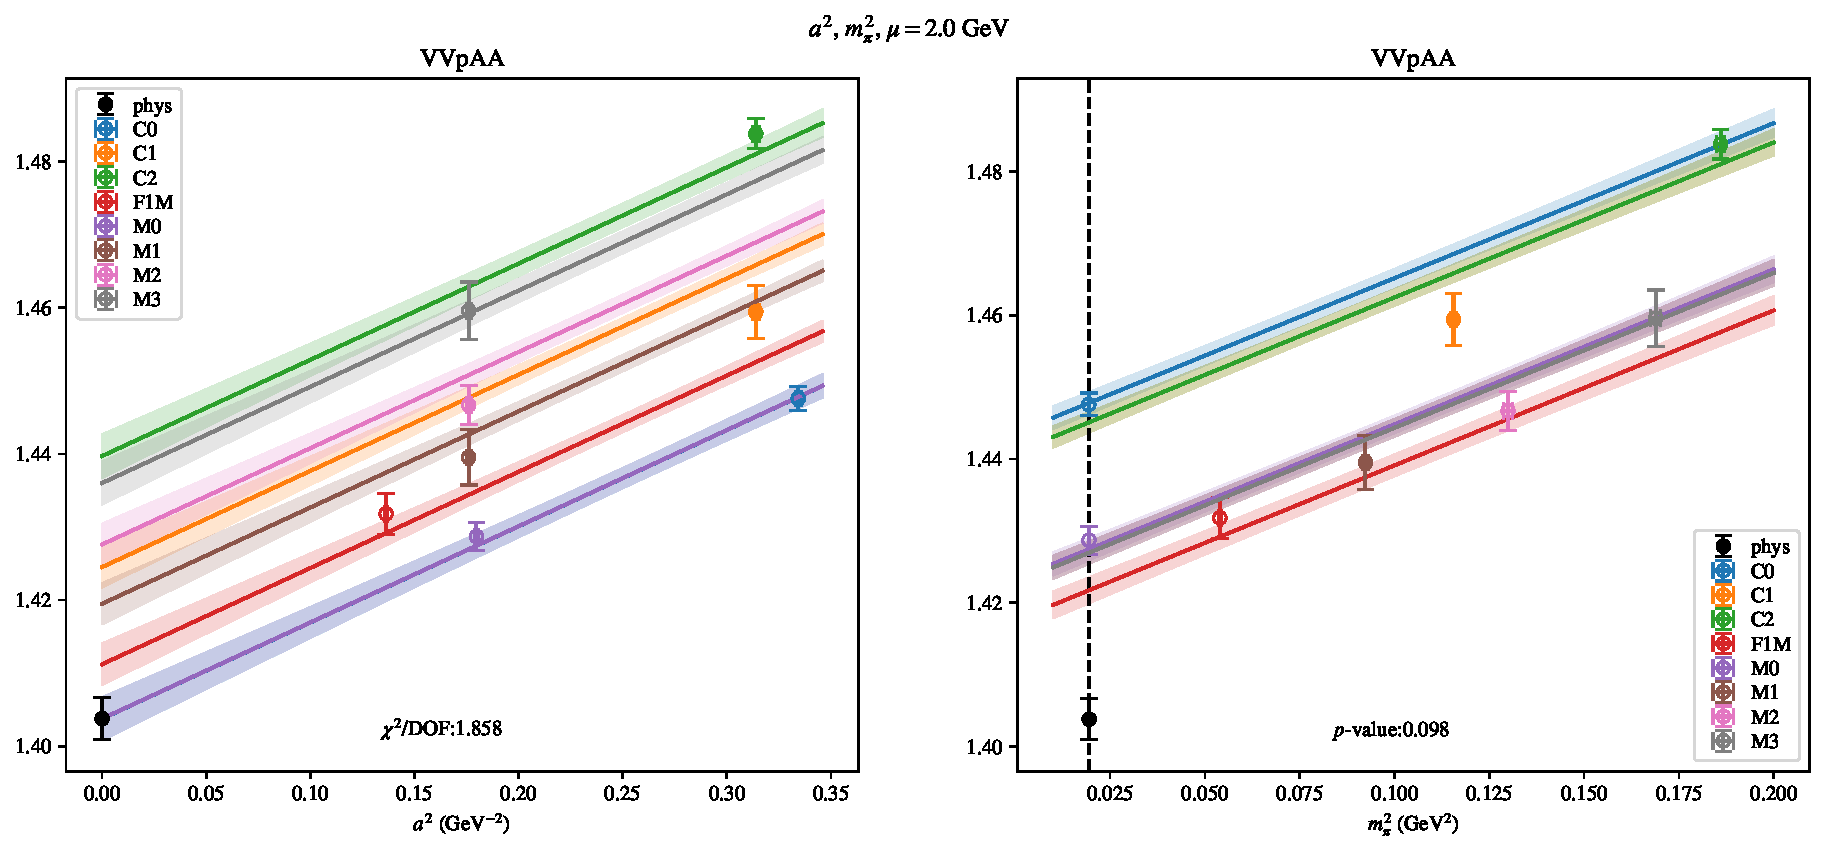
\includepdf[link, pages=-]{VVpAA/SUSY/a2m2_20.pdf}
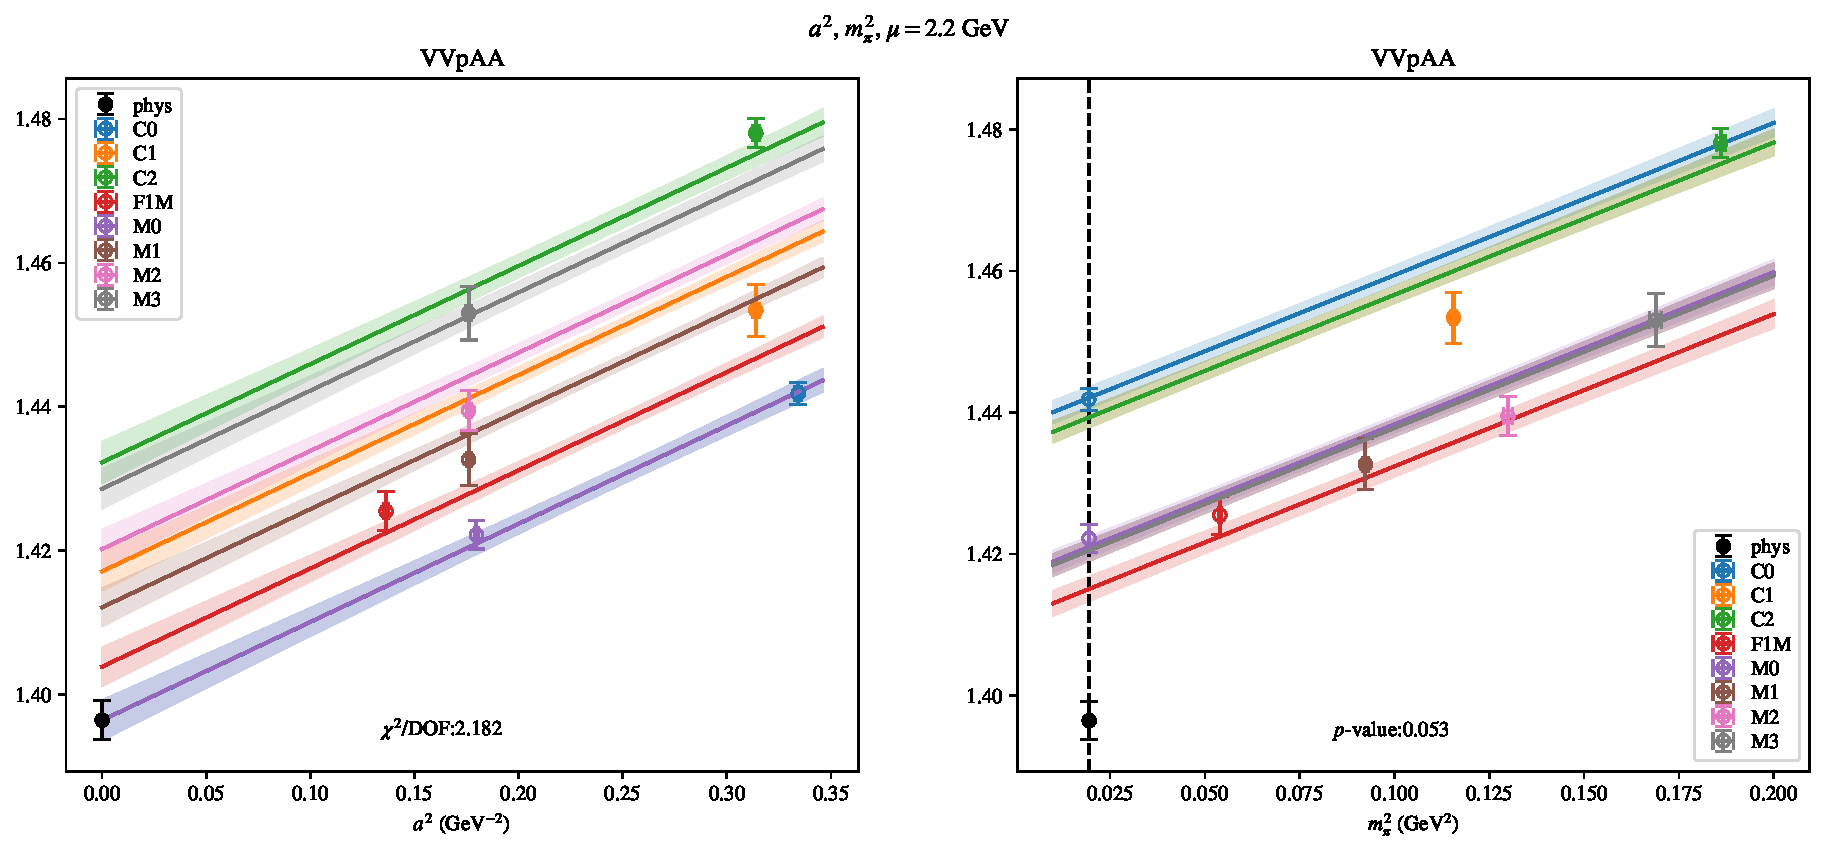
\includepdf[link, pages=-]{VVpAA/SUSY/a2m2_22.pdf}
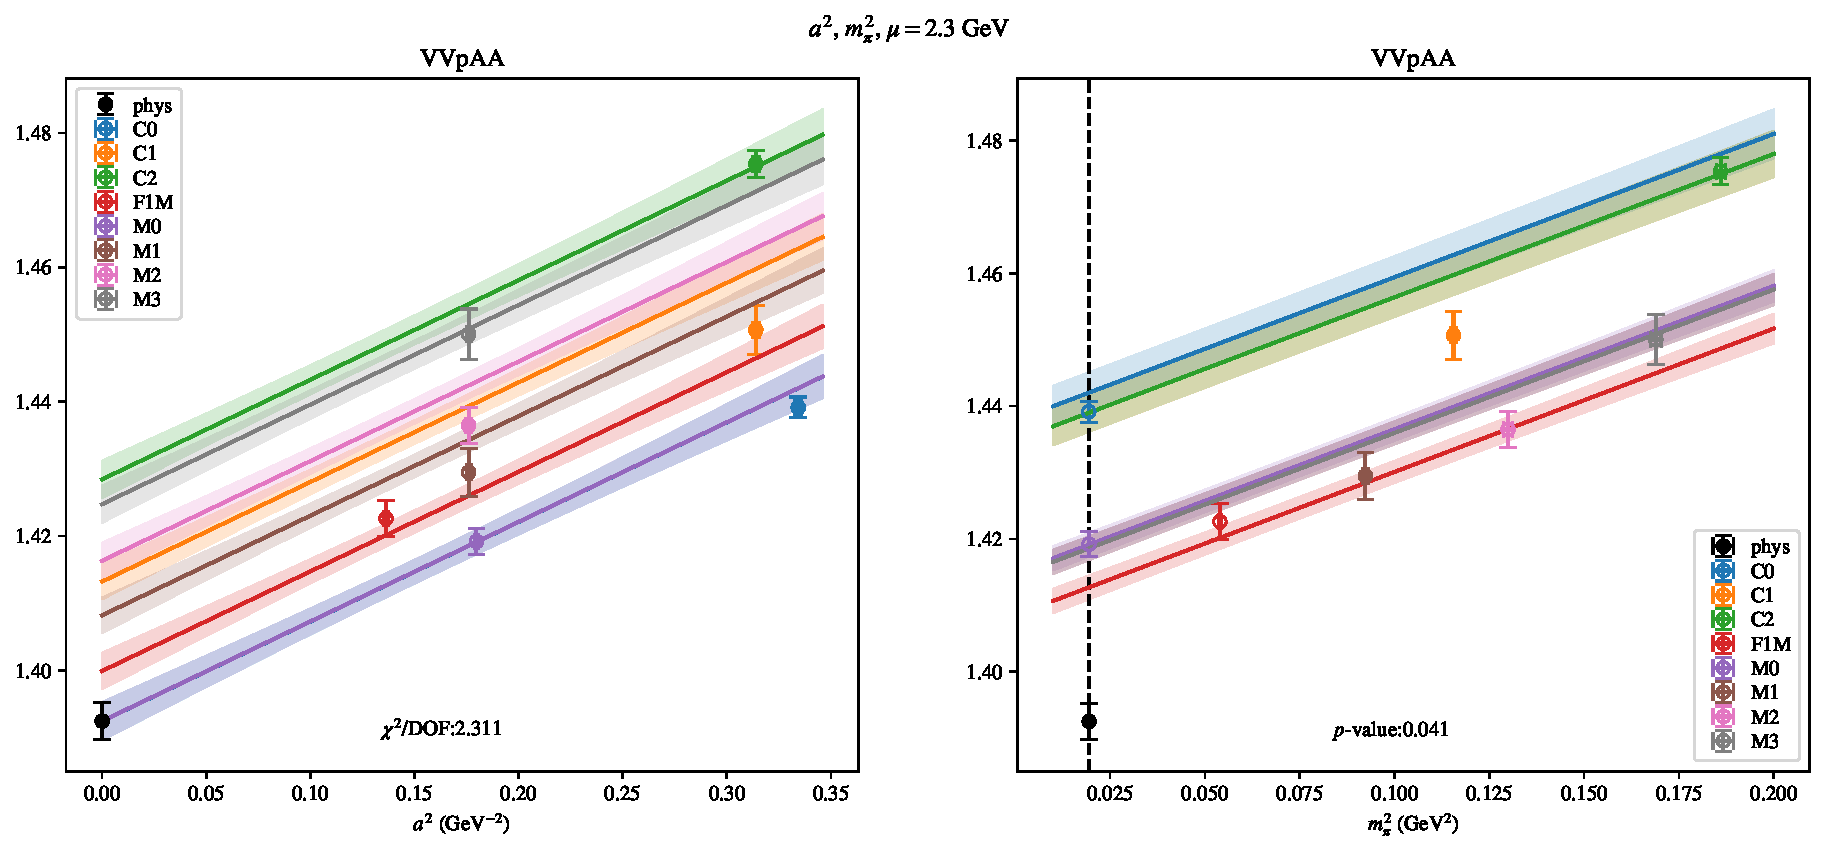
\includepdf[link, pages=-]{VVpAA/SUSY/a2m2_23.pdf}
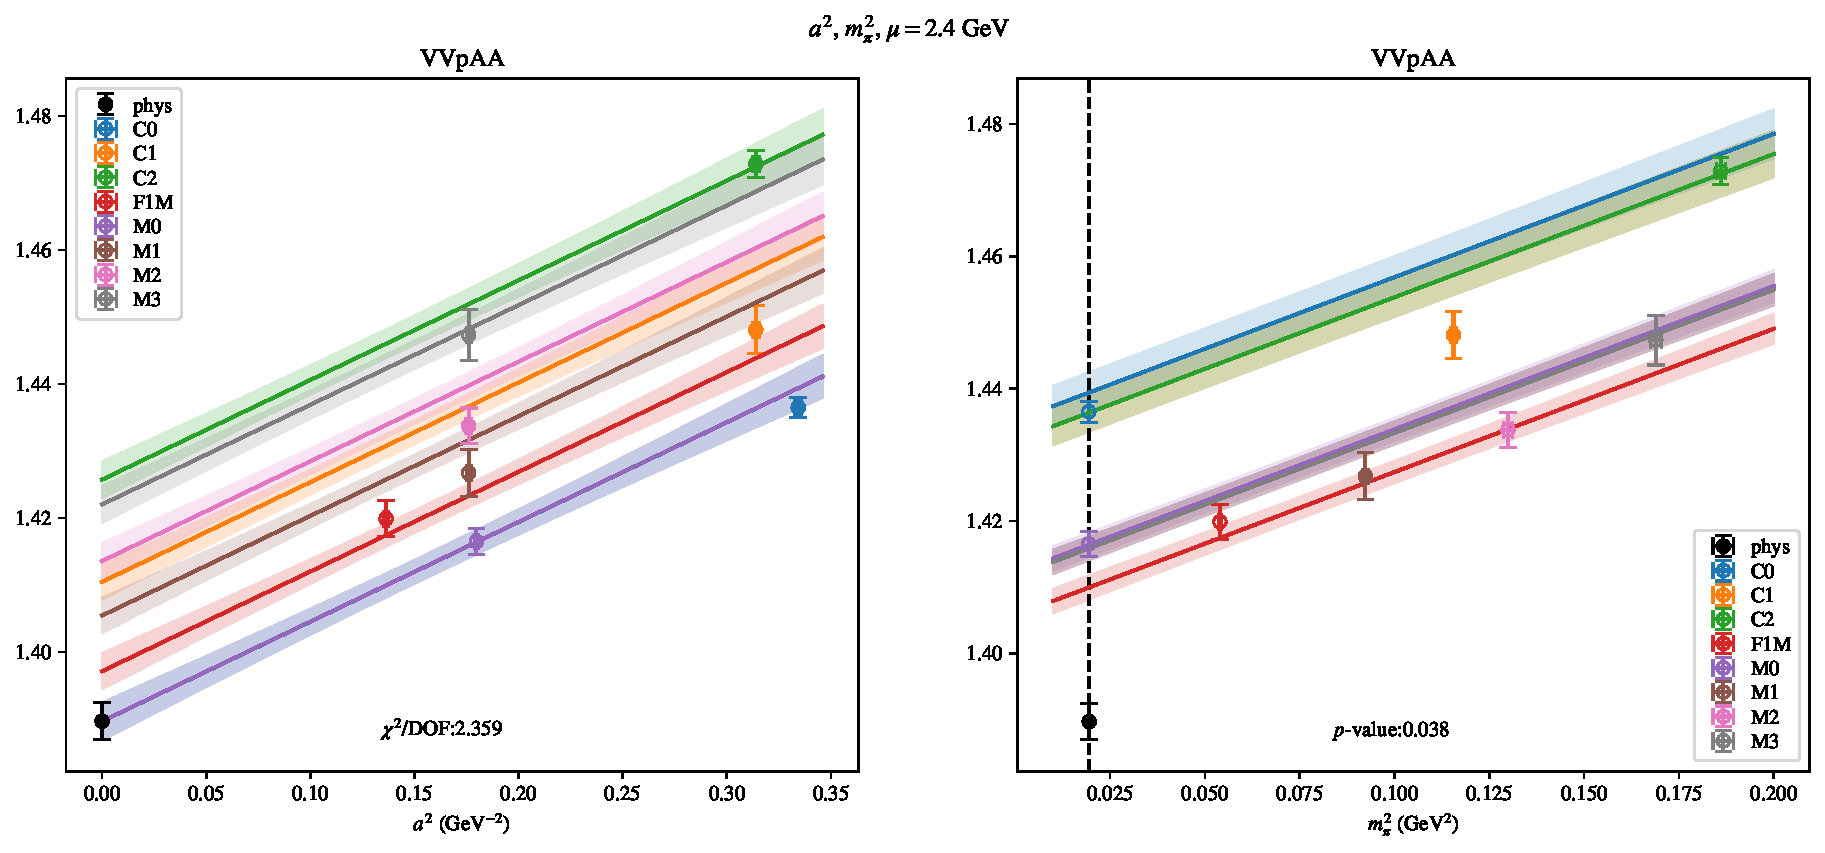
\includepdf[link, pages=-]{VVpAA/SUSY/a2m2_24.pdf}
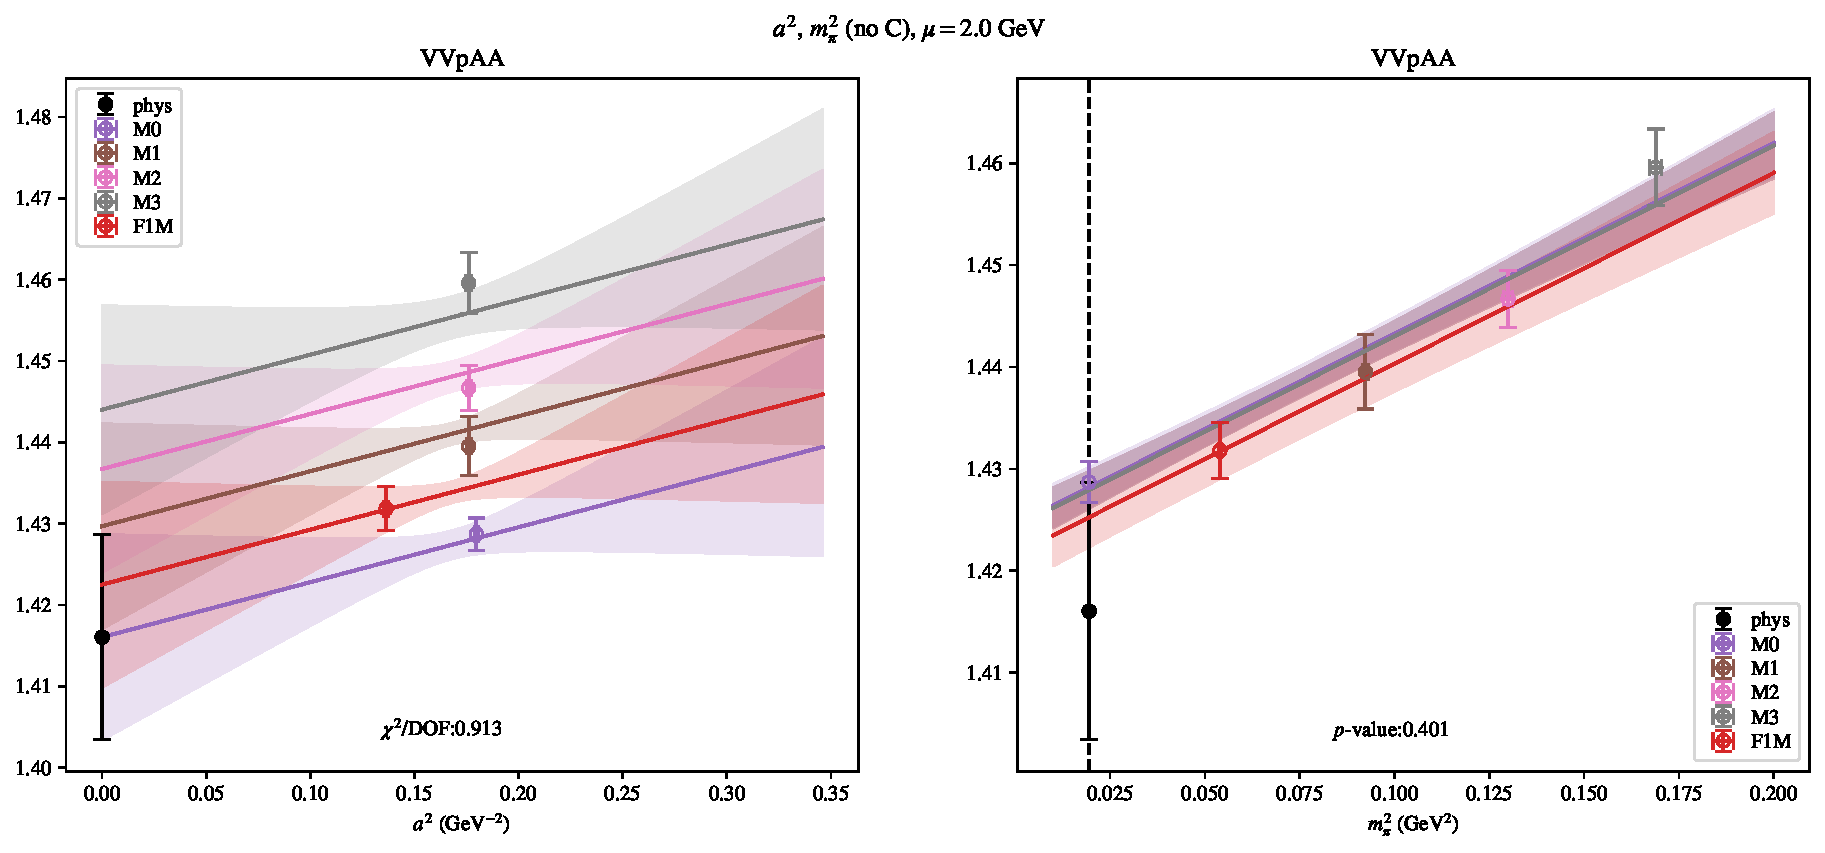
\includepdf[link, pages=-]{VVpAA/SUSY/a2m2noC_20.pdf}
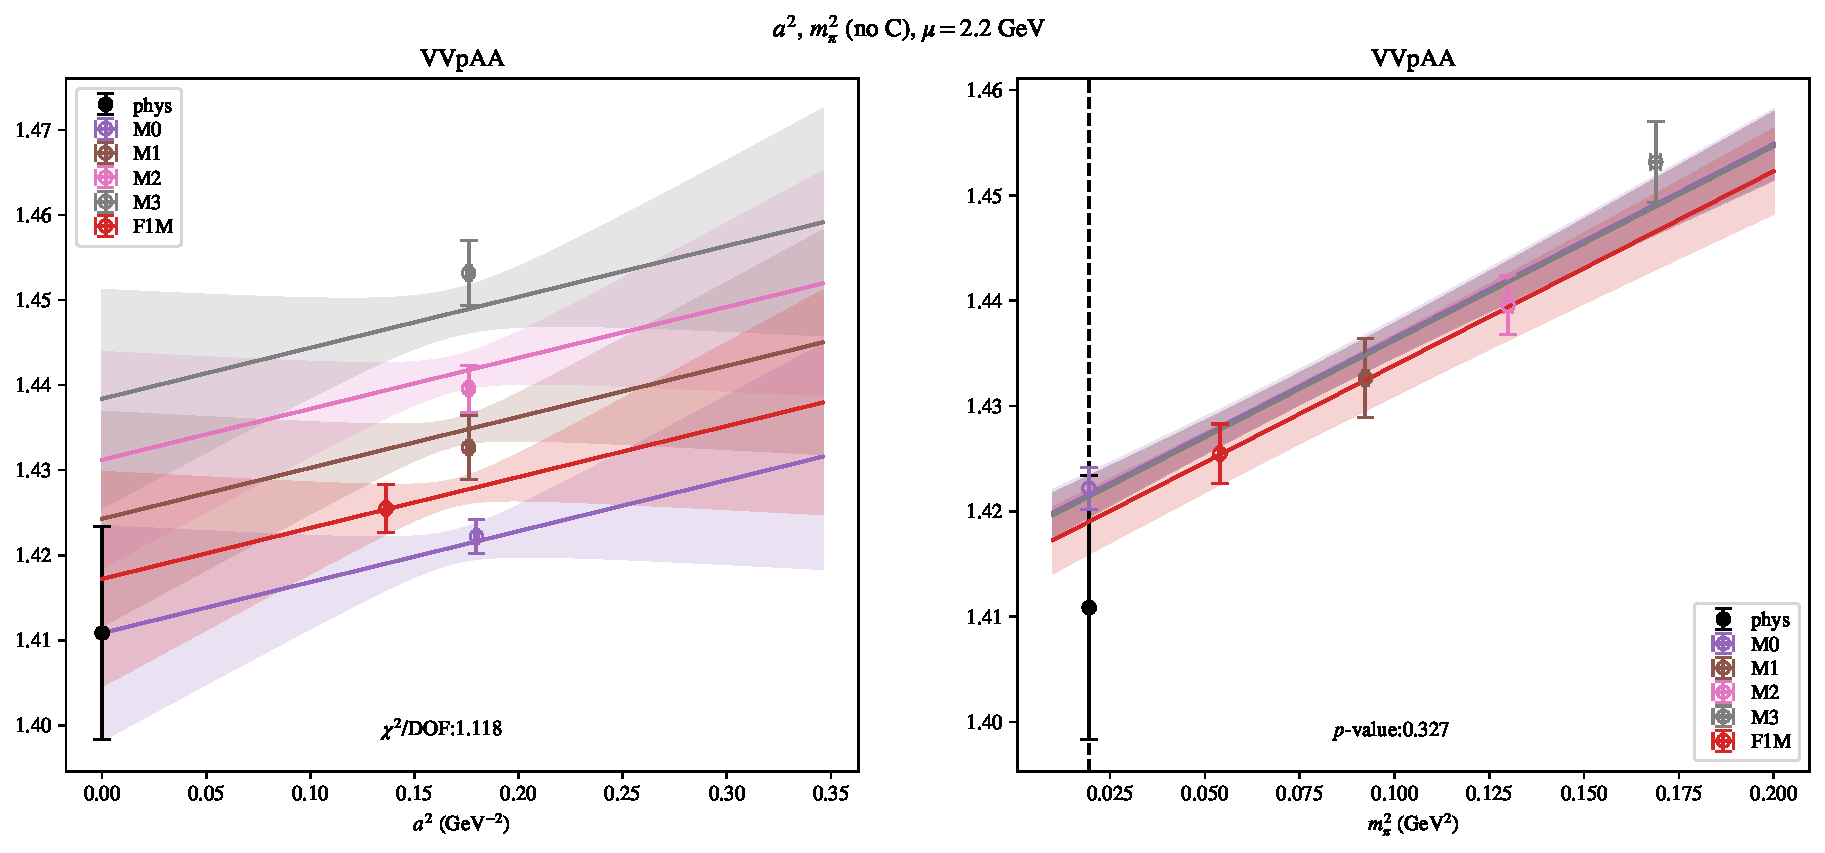
\includepdf[link, pages=-]{VVpAA/SUSY/a2m2noC_22.pdf}
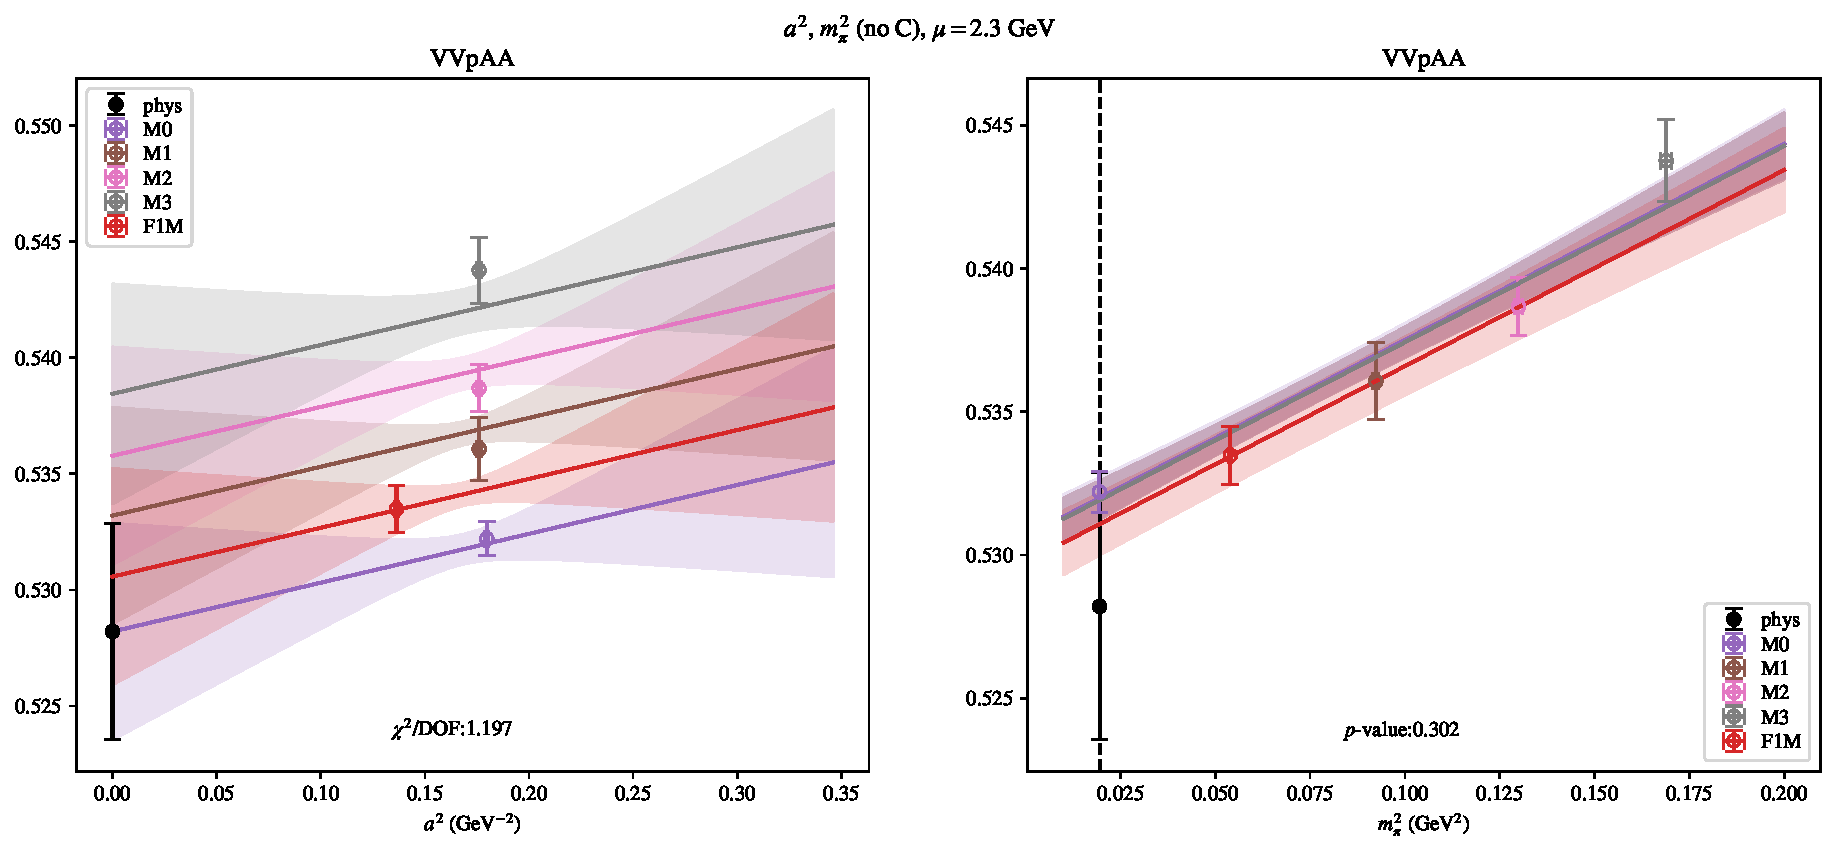
\includepdf[link, pages=-]{VVpAA/SUSY/a2m2noC_23.pdf}
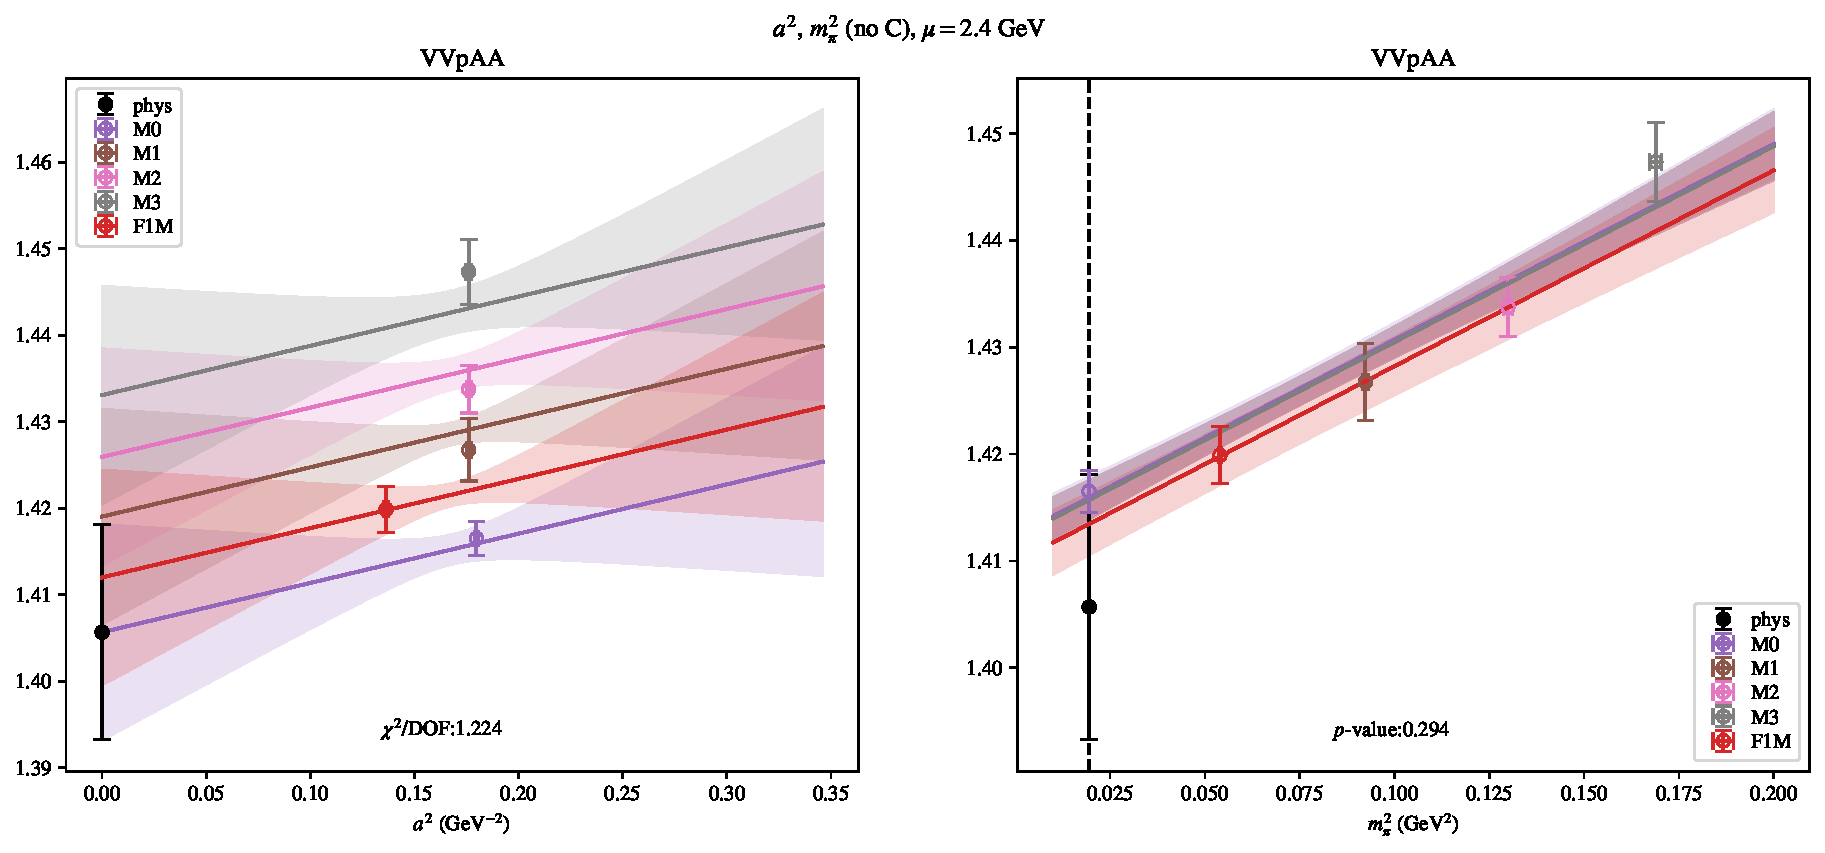
\includepdf[link, pages=-]{VVpAA/SUSY/a2m2noC_24.pdf}
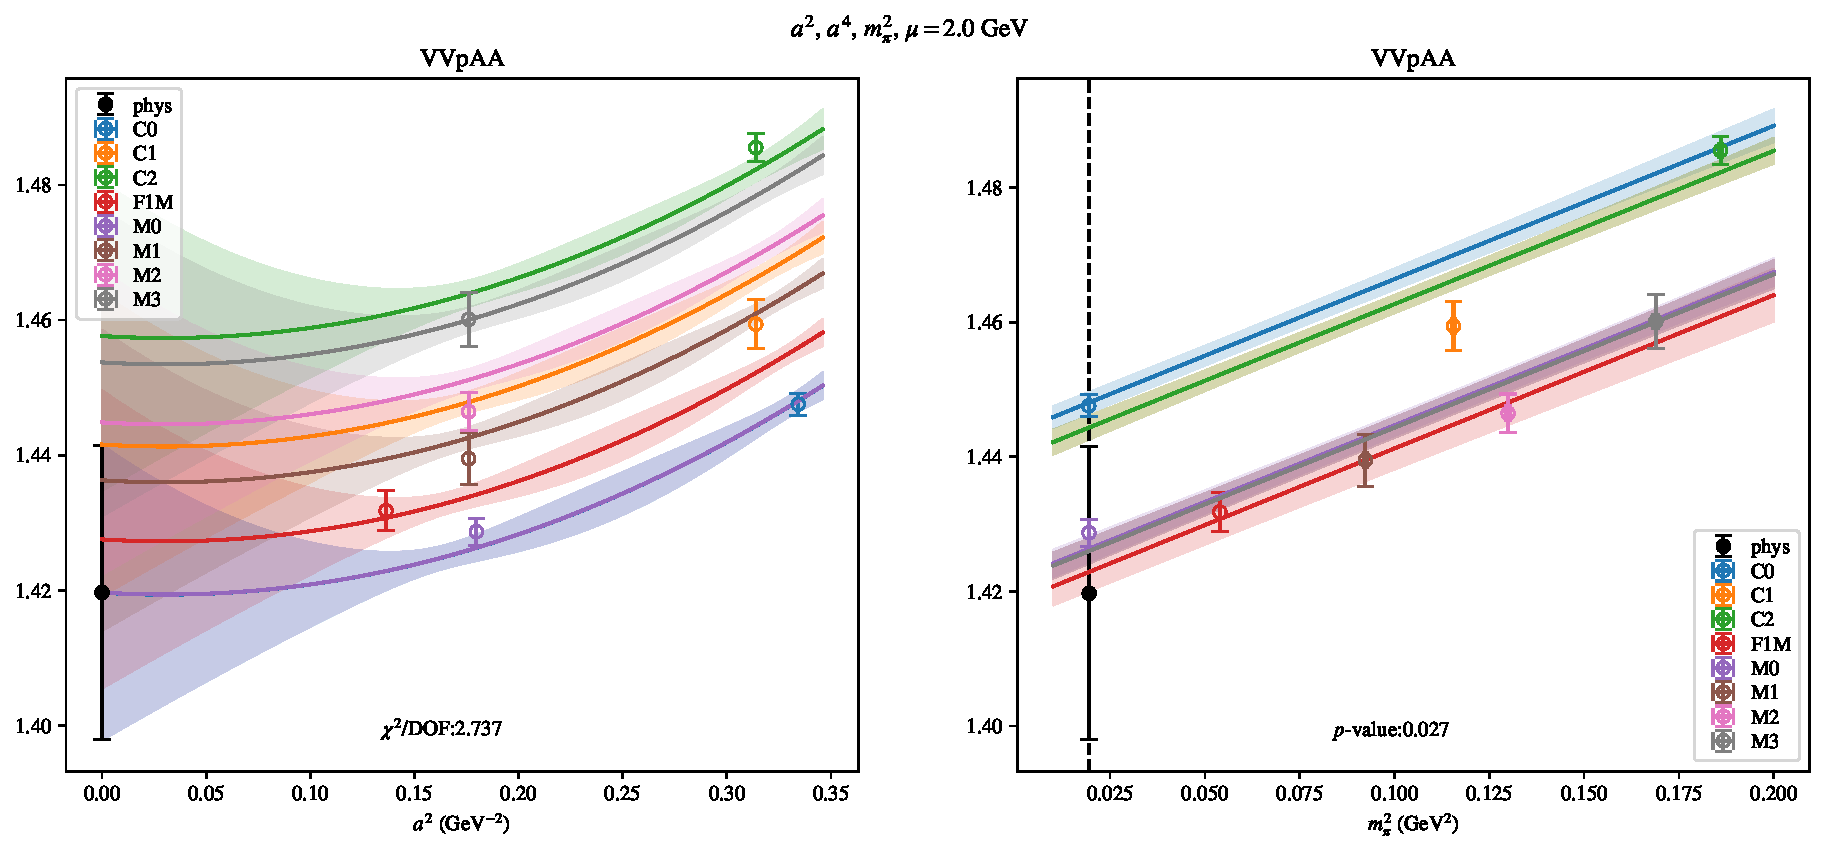
\includepdf[link, pages=-]{VVpAA/SUSY/a2a4m2_20.pdf}
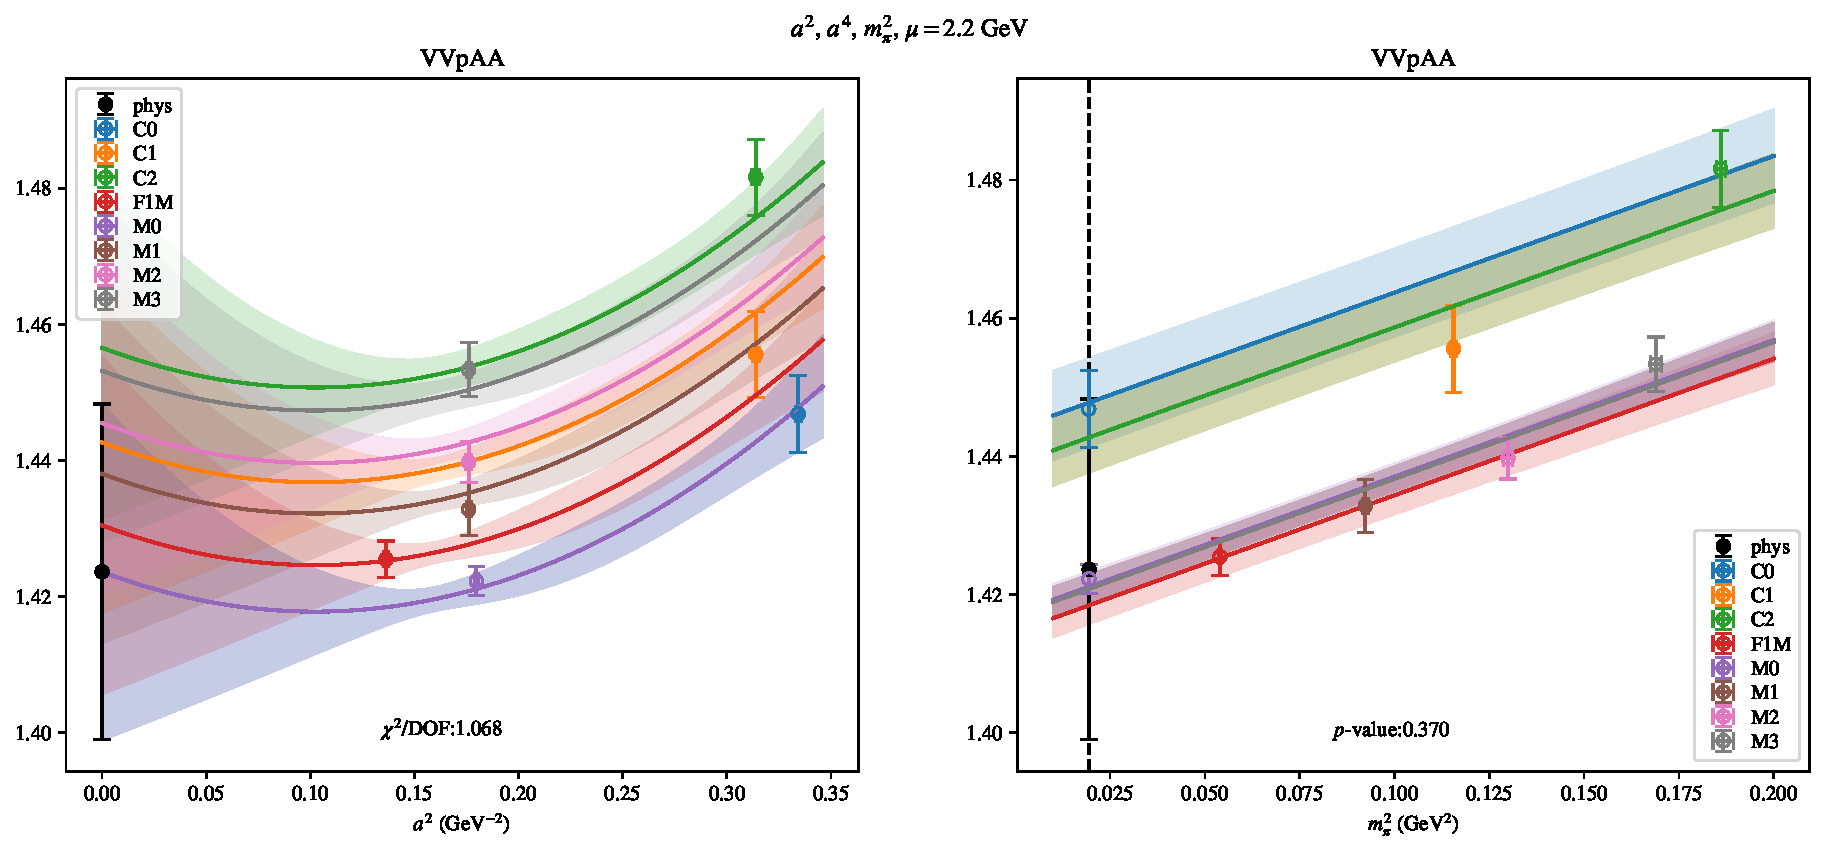
\includepdf[link, pages=-]{VVpAA/SUSY/a2a4m2_22.pdf}
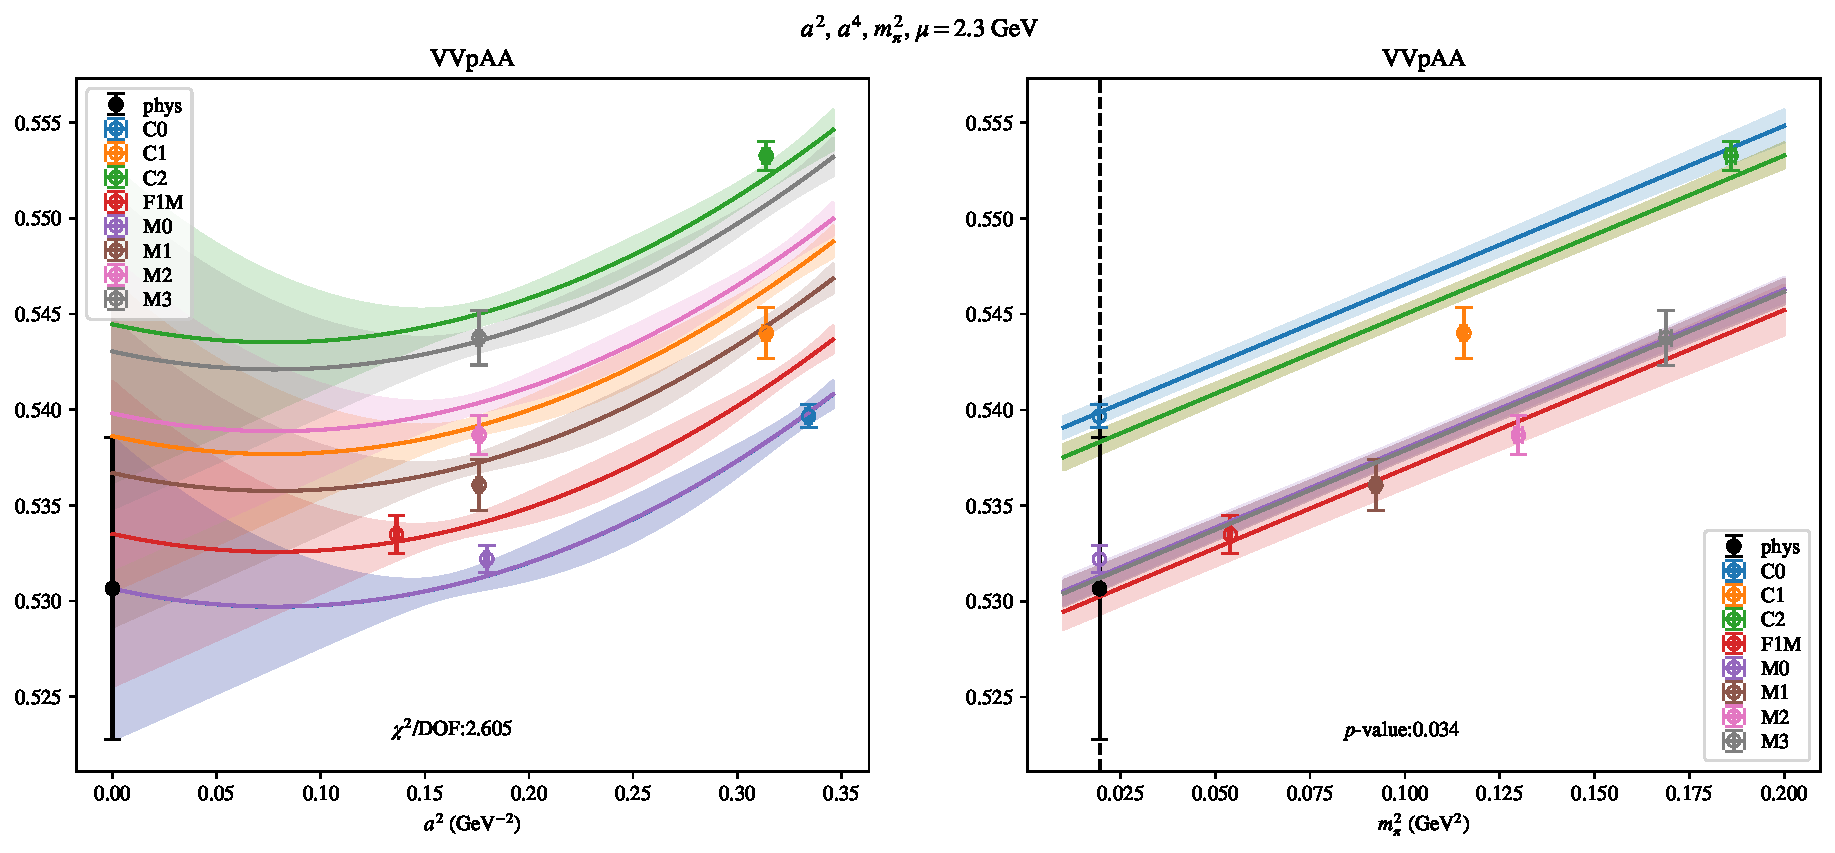
\includepdf[link, pages=-]{VVpAA/SUSY/a2a4m2_23.pdf}
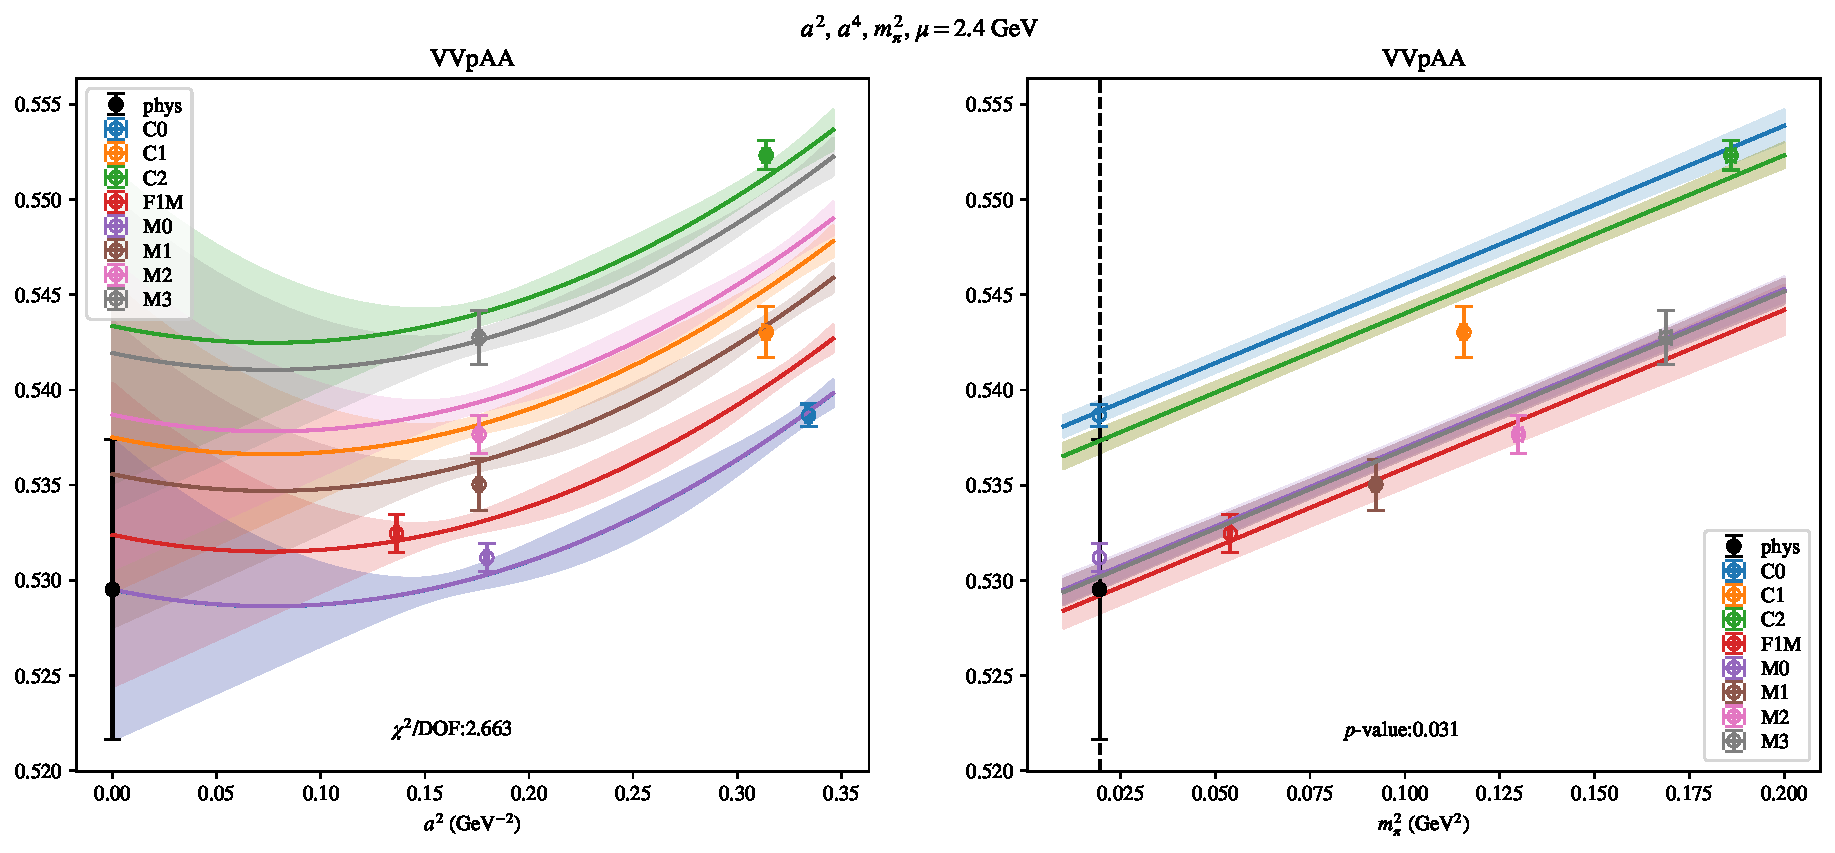
\includepdf[link, pages=-]{VVpAA/SUSY/a2a4m2_24.pdf}
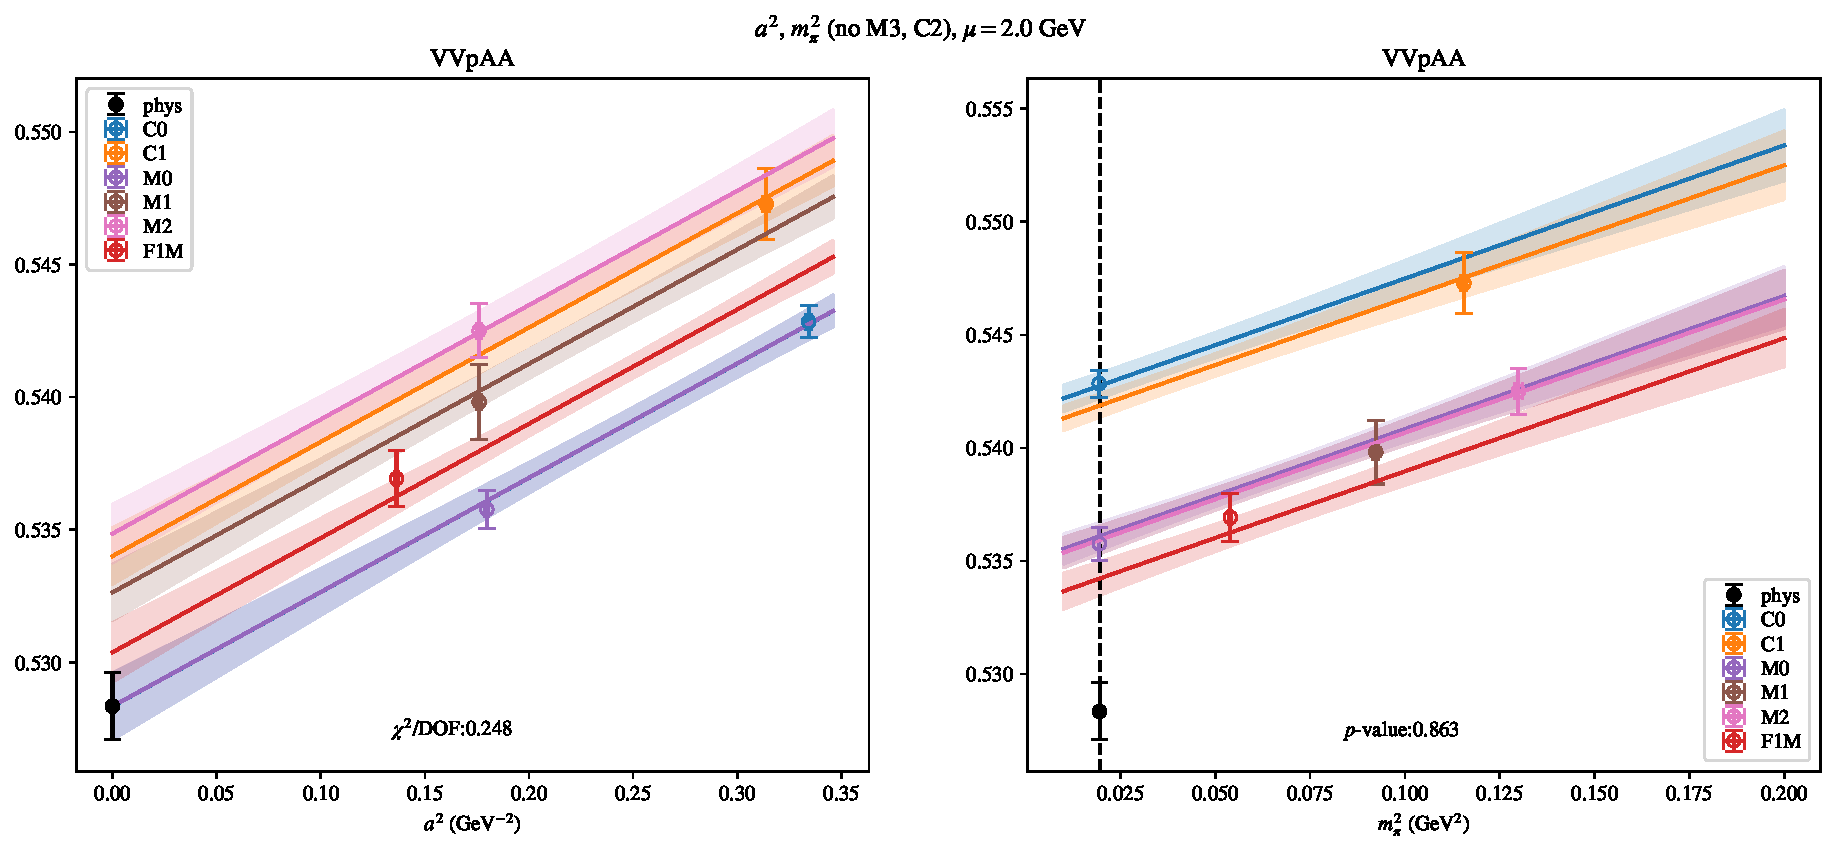
\includepdf[link, pages=-]{VVpAA/SUSY/a2m2mcut_20.pdf}
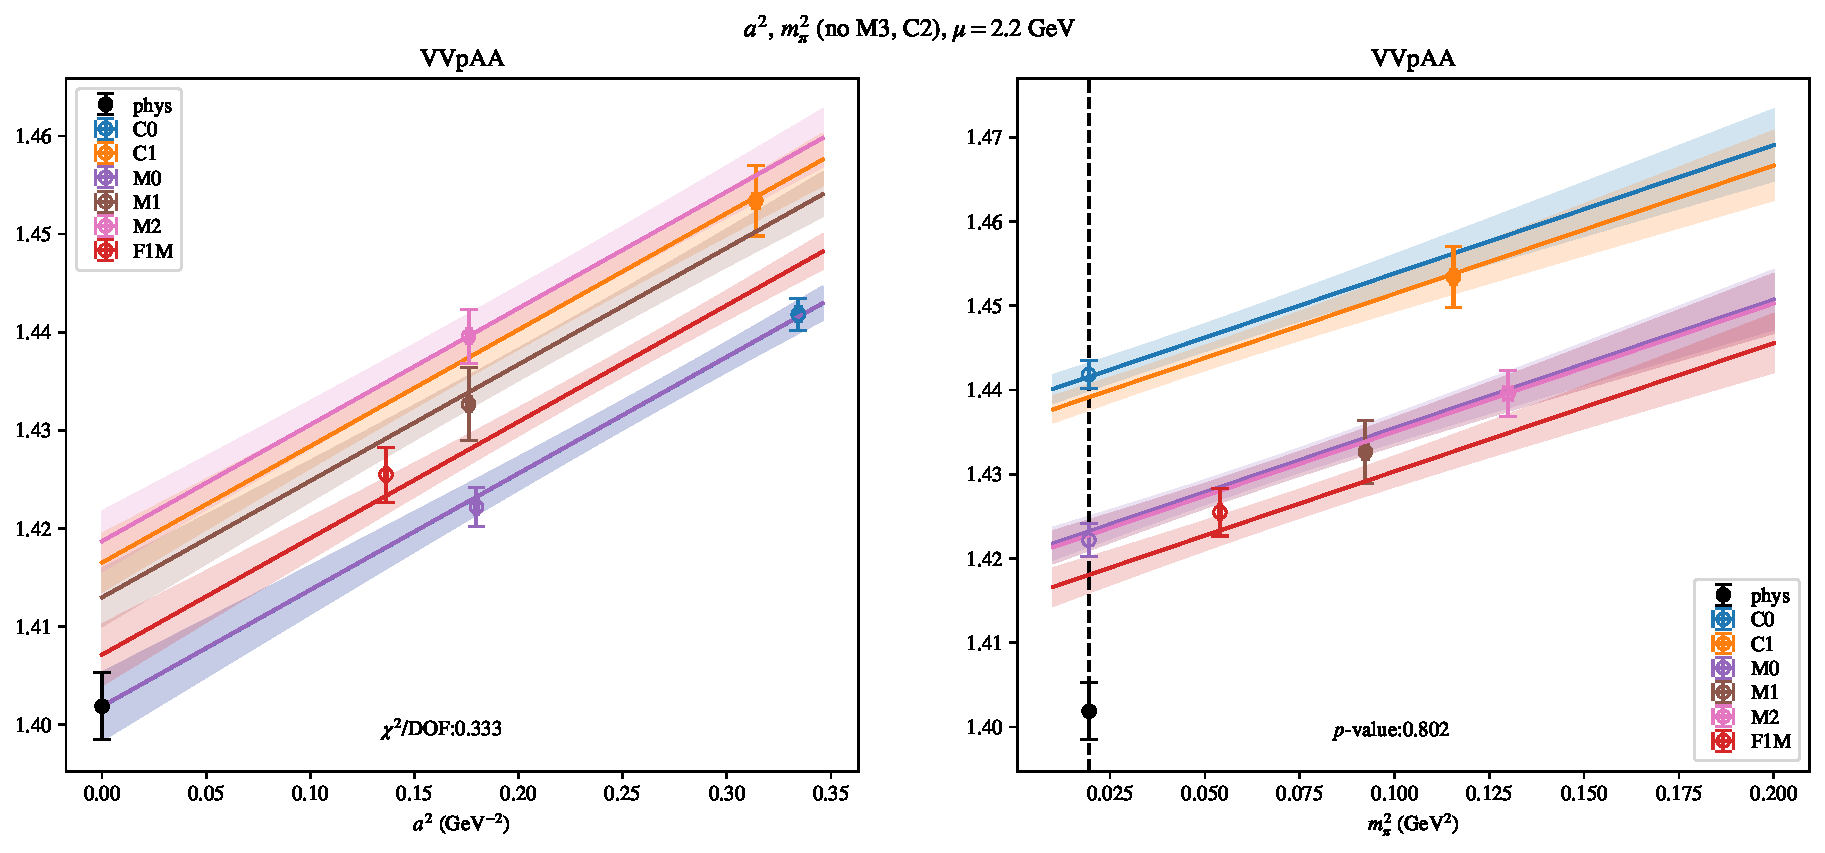
\includepdf[link, pages=-]{VVpAA/SUSY/a2m2mcut_22.pdf}
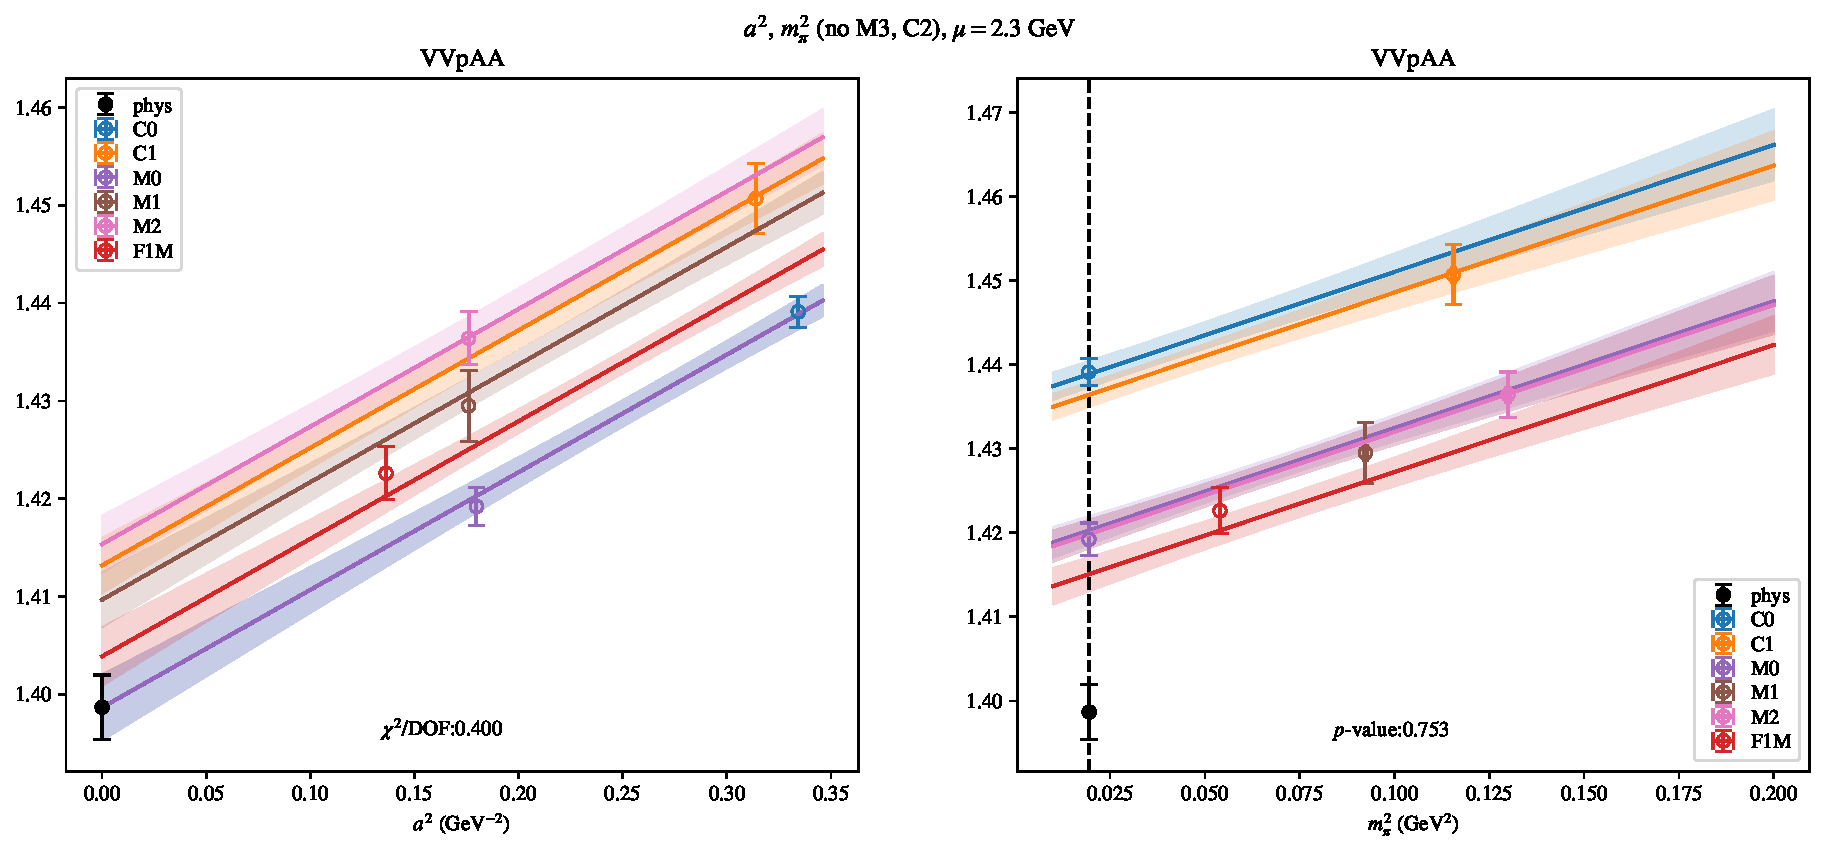
\includepdf[link, pages=-]{VVpAA/SUSY/a2m2mcut_23.pdf}
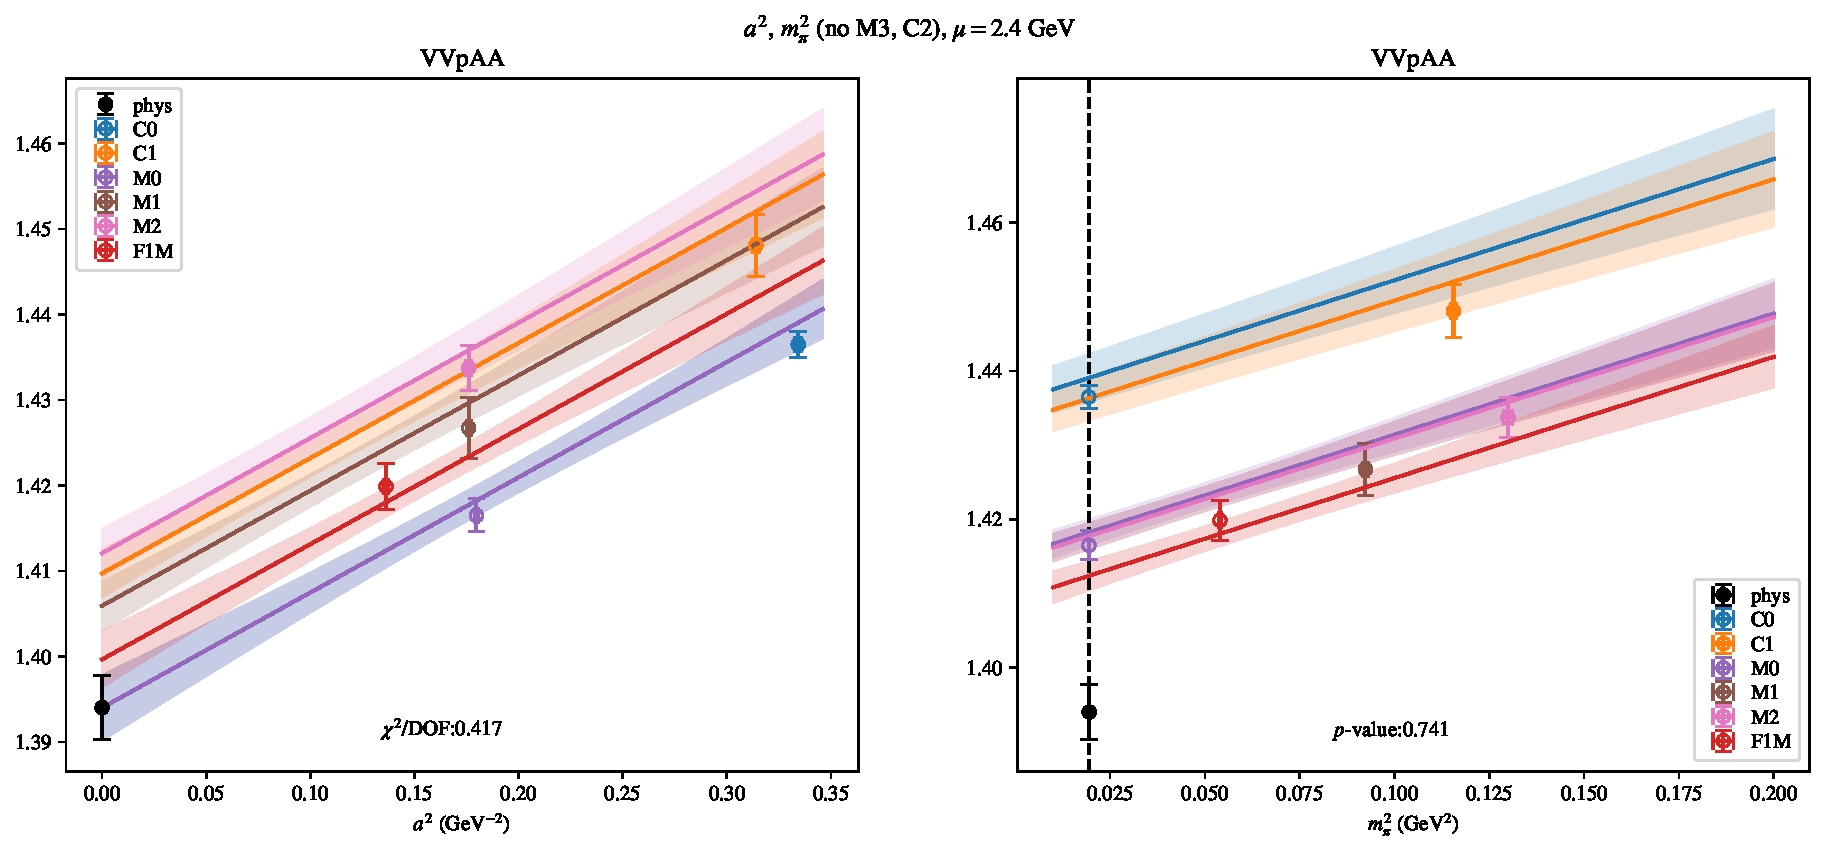
\includepdf[link, pages=-]{VVpAA/SUSY/a2m2mcut_24.pdf}
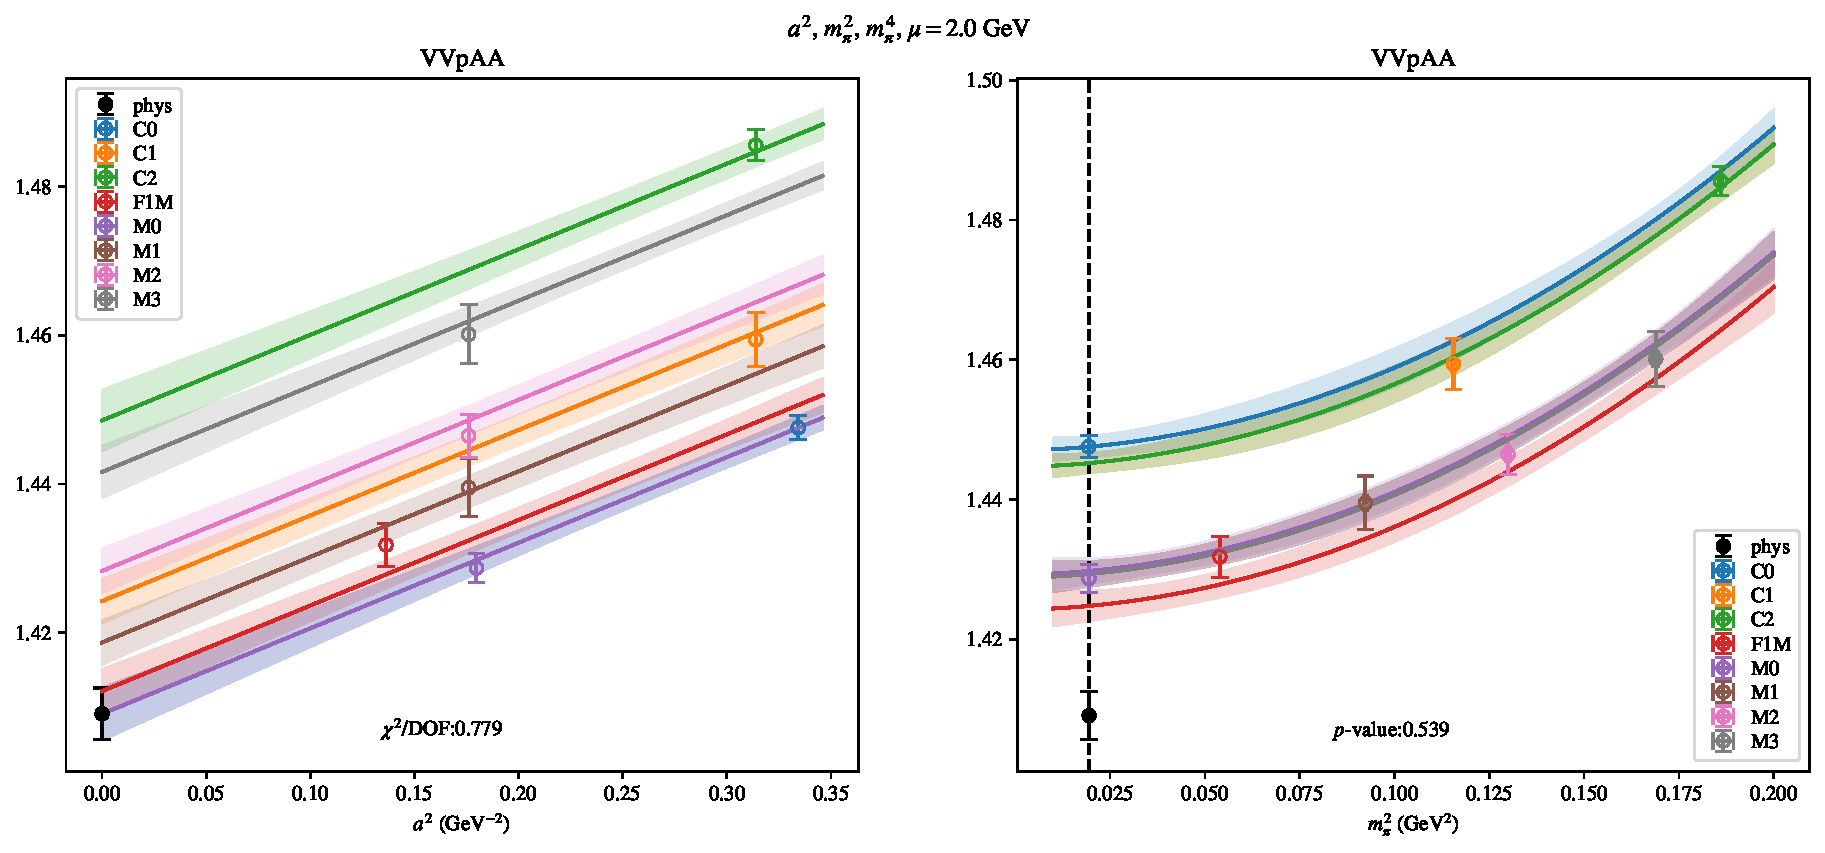
\includepdf[link, pages=-]{VVpAA/SUSY/a2m2m4_20.pdf}
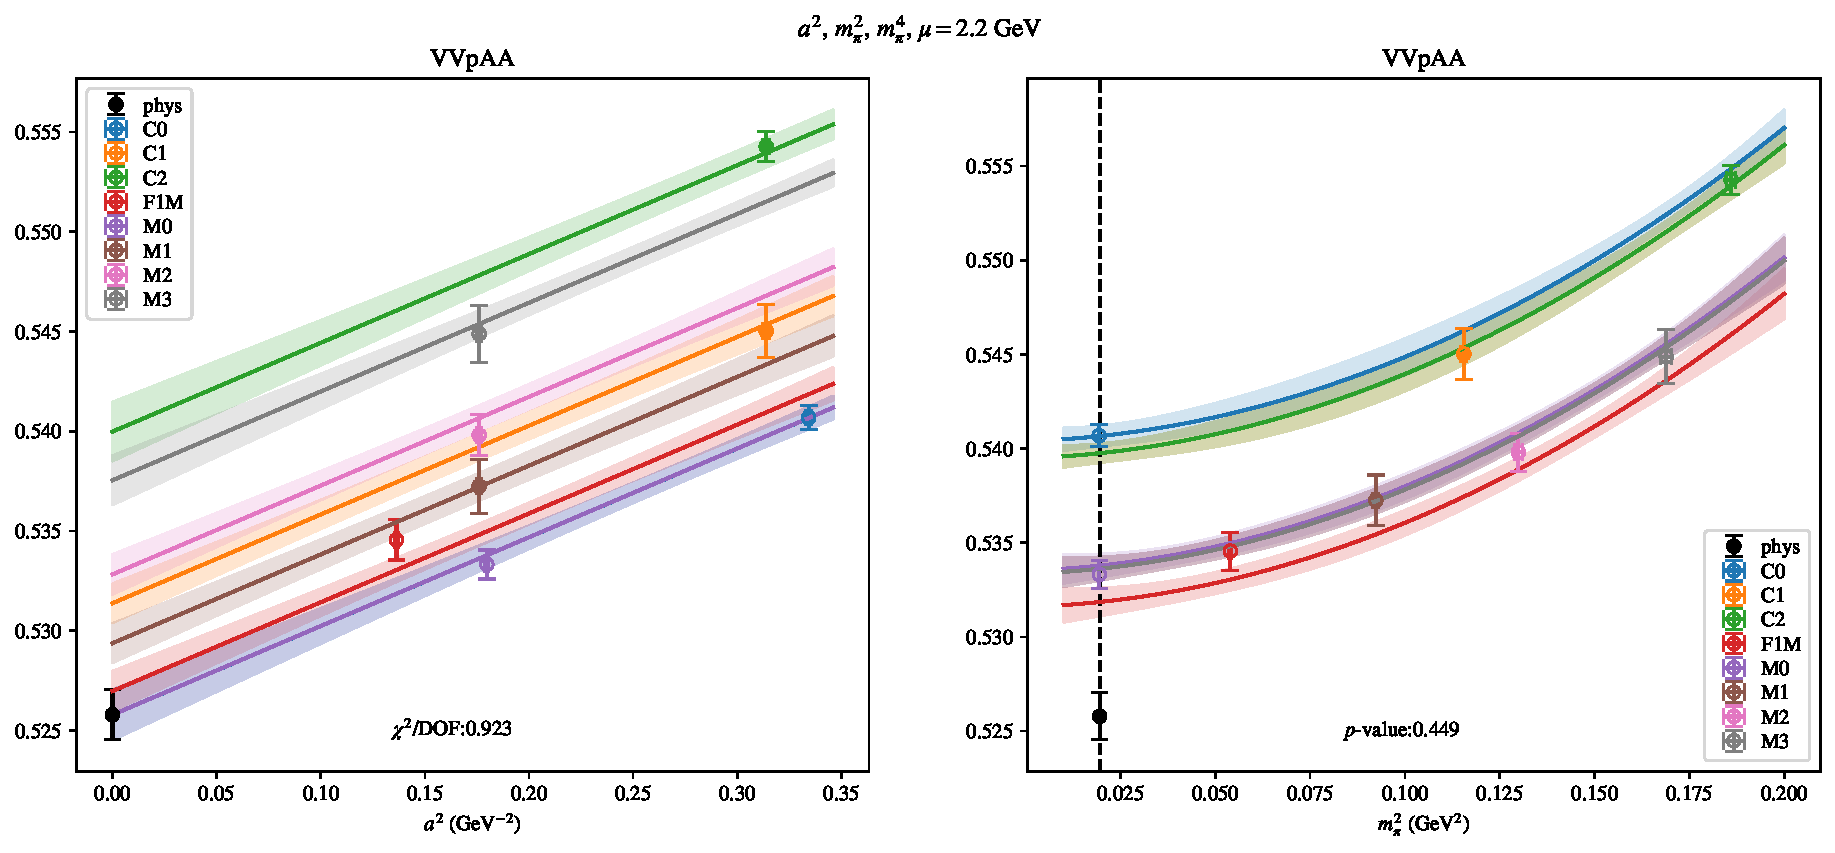
\includepdf[link, pages=-]{VVpAA/SUSY/a2m2m4_22.pdf}
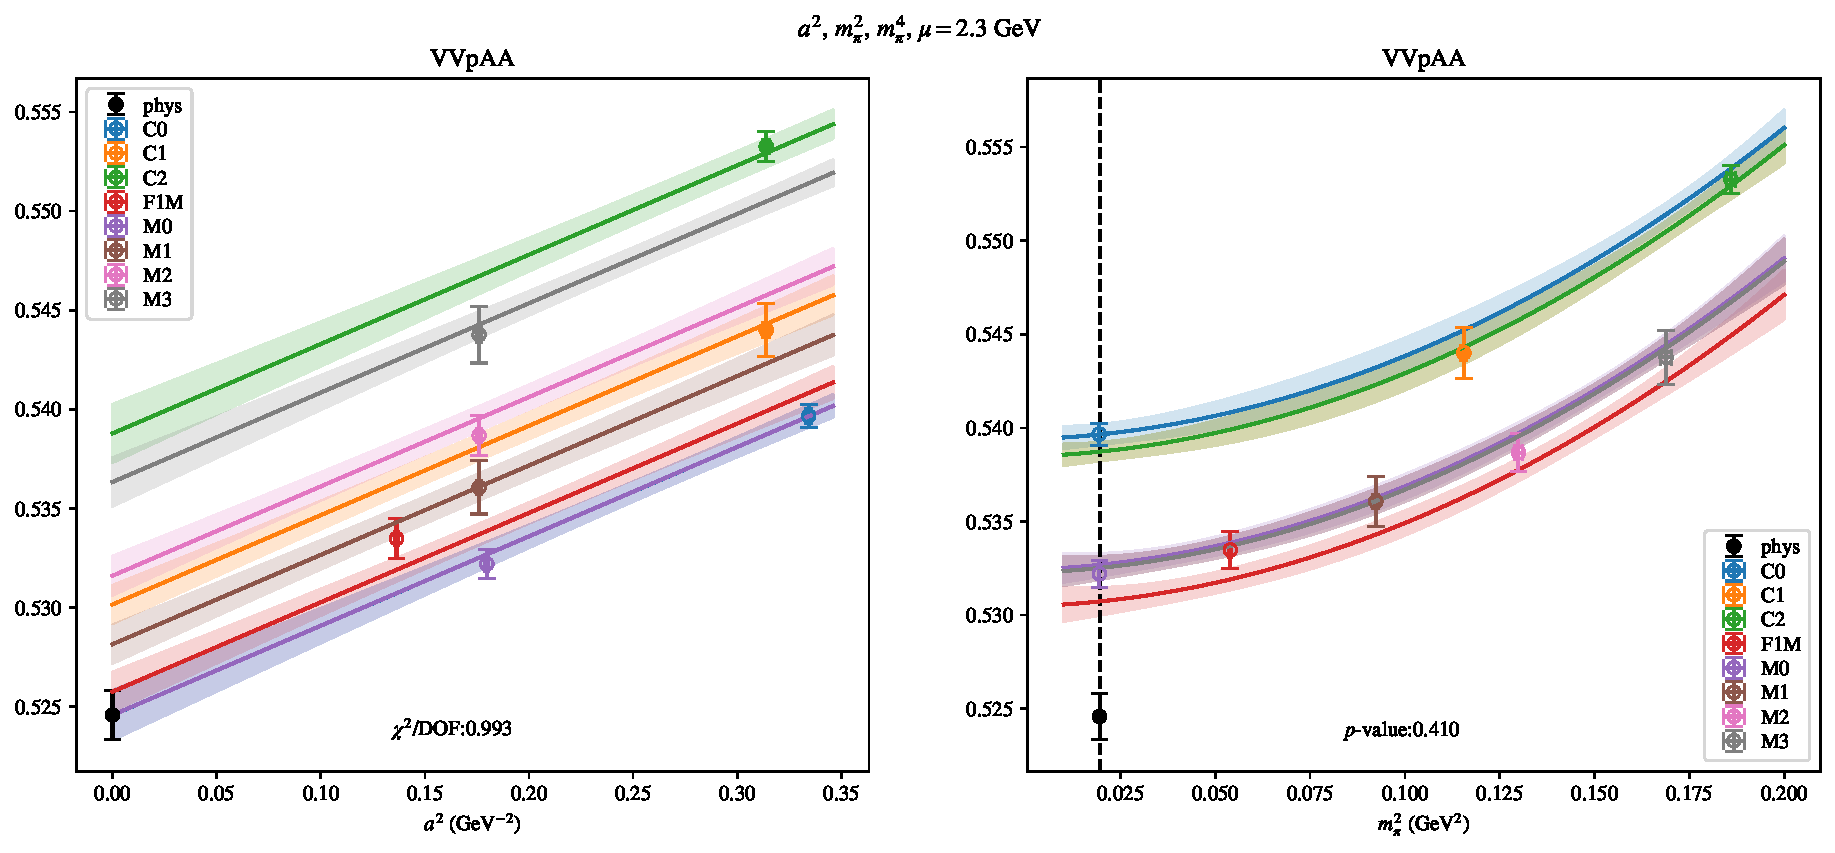
\includepdf[link, pages=-]{VVpAA/SUSY/a2m2m4_23.pdf}
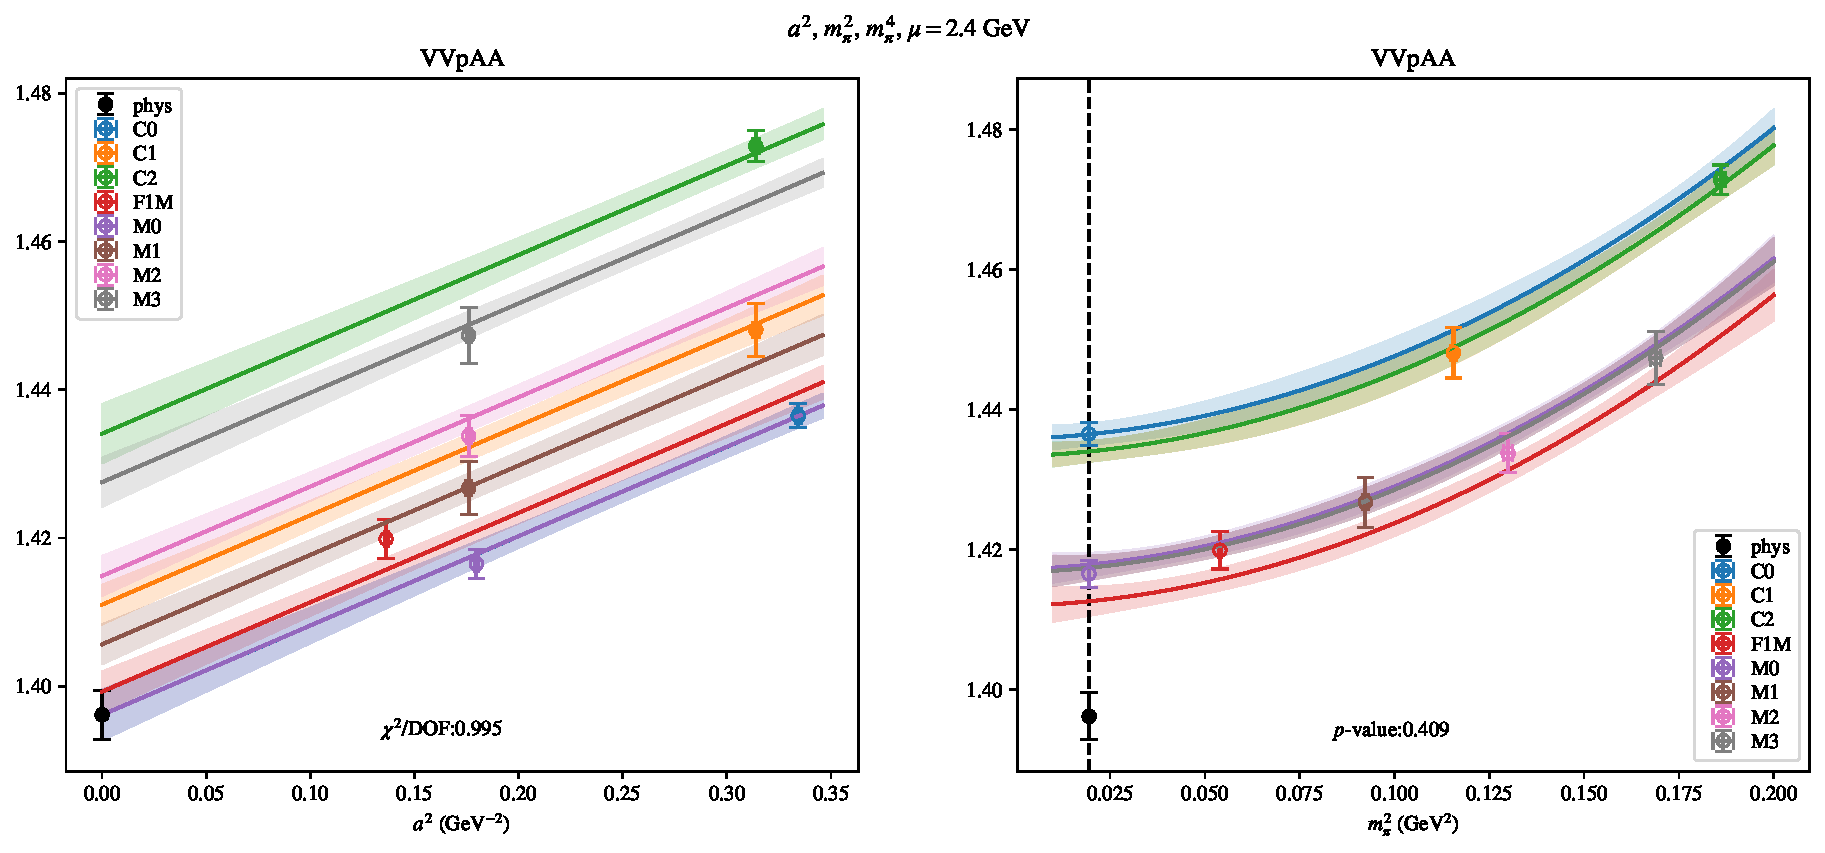
\includepdf[link, pages=-]{VVpAA/SUSY/a2m2m4_24.pdf}
\clearpage
\section{$\mathcal{B}_2$}
\begin{table}[h!]
\begin{center}
\begin{tabular}{|c|c|c|c|c|c|}
\hline
$\mu$ (GeV) & $a^2$, $m_\pi^2$& $a^2$, $m_\pi^2$ (no C)& $a^2$, $a^4$, $m_\pi^2$& $a^2$, $m_\pi^2$ (no M3, C2)& $a^2$, $m_\pi^2$, $m_\pi^4$\\
\hline
2.0& \hyperlink{VVmAA/SUSY/a2m2_20.pdf.1}{\textbf{-0.925(16)}: 2.885 (0.013)} & \hyperlink{VVmAA/SUSY/a2m2noC_20.pdf.1}{\textbf{-0.936(95)}: 2.412 (0.09)} & \hyperlink{VVmAA/SUSY/a2a4m2_20.pdf.1}{\textbf{-0.92(16)}: 3.607 (0.006)} & \hyperlink{VVmAA/SUSY/a2m2mcut_20.pdf.1}{\textbf{-0.925(19)}: 3.122 (0.025)} & \hyperlink{VVmAA/SUSY/a2m2m4_20.pdf.1}{\textbf{-0.924(18)}: 2.59 (0.035)}\\
2.2& \hyperlink{VVmAA/SUSY/a2m2_22.pdf.1}{\textbf{-0.905(16)}: 3.937 (0.001)} & \hyperlink{VVmAA/SUSY/a2m2noC_22.pdf.1}{\textbf{-0.920(90)}: 1.967 (0.14)} & \hyperlink{VVmAA/SUSY/a2a4m2_22.pdf.1}{\textbf{-0.90(15)}: 4.921 (0.001)} & \hyperlink{VVmAA/SUSY/a2m2mcut_22.pdf.1}{\textbf{-0.906(18)}: 4.12 (0.006)} & \hyperlink{VVmAA/SUSY/a2m2m4_22.pdf.1}{\textbf{-0.904(18)}: 4.142 (0.002)}\\
2.3& \hyperlink{VVmAA/SUSY/a2m2_23.pdf.1}{\textbf{-0.897(16)}: 4.405 (0.001)} & \hyperlink{VVmAA/SUSY/a2m2noC_23.pdf.1}{\textbf{-0.913(88)}: 2.284 (0.102)} & \hyperlink{VVmAA/SUSY/a2a4m2_23.pdf.1}{\textbf{-0.90(15)}: 5.494 (0.0)} & \hyperlink{VVmAA/SUSY/a2m2mcut_23.pdf.1}{\textbf{-0.897(18)}: 4.775 (0.002)} & \hyperlink{VVmAA/SUSY/a2m2m4_23.pdf.1}{\textbf{-0.895(18)}: 4.544 (0.001)}\\
2.4& \hyperlink{VVmAA/SUSY/a2m2_24.pdf.1}{\textbf{-0.889(16)}: 4.799 (0.0)} & \hyperlink{VVmAA/SUSY/a2m2noC_24.pdf.1}{\textbf{-0.906(88)}: 2.427 (0.088)} & \hyperlink{VVmAA/SUSY/a2a4m2_24.pdf.1}{\textbf{-0.89(15)}: 5.991 (0.0)} & \hyperlink{VVmAA/SUSY/a2m2mcut_24.pdf.1}{\textbf{-0.890(18)}: 5.334 (0.001)} & \hyperlink{VVmAA/SUSY/a2m2m4_24.pdf.1}{\textbf{-0.887(18)}: 5.056 (0.0)}\\
\hline
\end{tabular}
\caption{Physical point value from chiral and continuum extrapolation at renormalisation scale $\mu$. Entries are \textbf{value(error)}: $\chi^2/\text{DOF}$ ($p$-value).}
\end{center}
\end{table}
\begin{table}[h!]
\begin{center}
\begin{tabular}{|c c|c|c|c|c|c|}
\hline
$\mu$ (GeV) &  & $a^2$, $m_\pi^2$& $a^2$, $m_\pi^2$ (no C)& $a^2$, $a^4$, $m_\pi^2$& $a^2$, $m_\pi^2$ (no M3, C2)& $a^2$, $m_\pi^2$, $m_\pi^4$\\
\hline
\multirow{2}{0.5in}{2.0} & $\alpha$ & 0.3754(77)& 0.308(62)& 0.37(16)& 0.3753(87)& 0.3815(85)\\
 & $\beta$ & 0.00665(15)& 0.00613(29)& 0.00665(16)& 0.00705(26)& 0.00838(81)\\
\hline
\multirow{2}{0.5in}{2.2} & $\alpha$ & 0.4227(79)& 0.330(60)& 0.41(16)& 0.4192(88)& 0.4280(86)\\
 & $\beta$ & 0.00705(15)& 0.00635(24)& 0.00705(16)& 0.00738(25)& 0.00849(75)\\
\hline
\multirow{2}{0.5in}{2.3} & $\alpha$ & 0.4443(79)& 0.339(59)& 0.41(16)& 0.4411(89)& 0.4504(87)\\
 & $\beta$ & 0.00714(15)& 0.00644(23)& 0.00713(16)& 0.00749(25)& 0.00871(75)\\
\hline
\multirow{2}{0.5in}{2.4} & $\alpha$ & 0.4634(80)& 0.355(60)& 0.43(16)& 0.4599(90)& 0.4695(88)\\
 & $\beta$ & 0.00724(15)& 0.00651(22)& 0.00723(16)& 0.00756(25)& 0.00877(75)\\
\hline
\end{tabular}
\caption{Fit values of coefficients in $Q = Q_{phys} + \mathbf{\alpha} a^2 + \mathbf{\beta}\left(\frac{m_\pi^2}{f_\pi^2}-\frac{m_{\pi,PDG}^2}{f_\pi^2}\right) + \ldots$.}
\end{center}
\end{table}
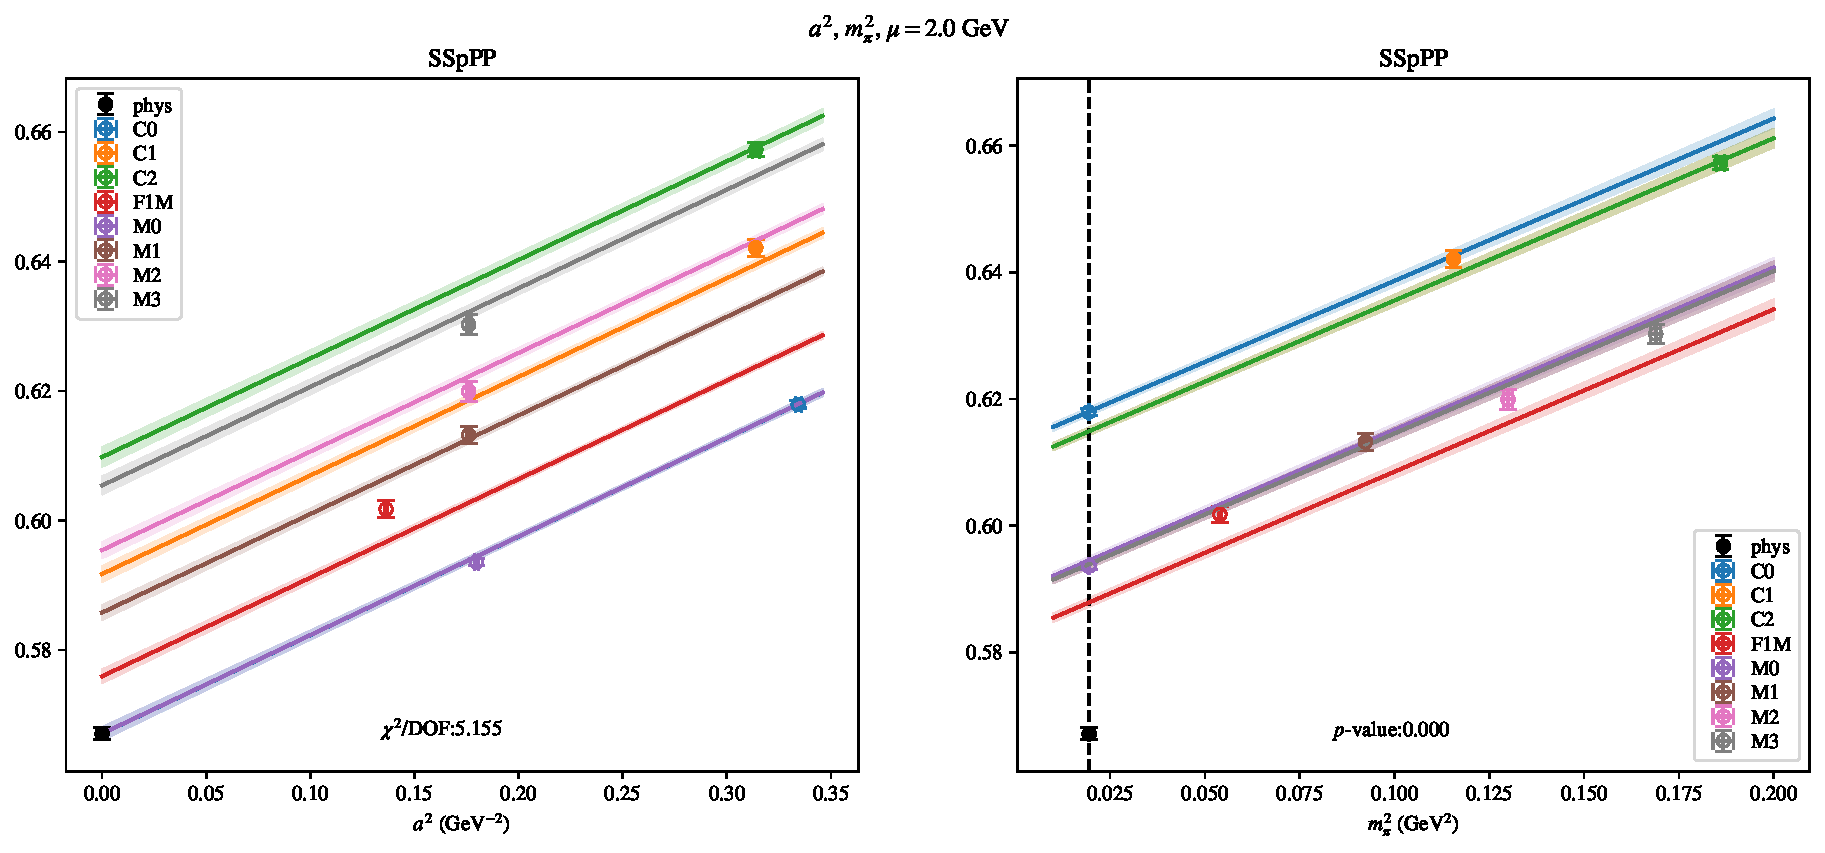
\includepdf[link, pages=-]{VVmAA/SUSY/a2m2_20.pdf}
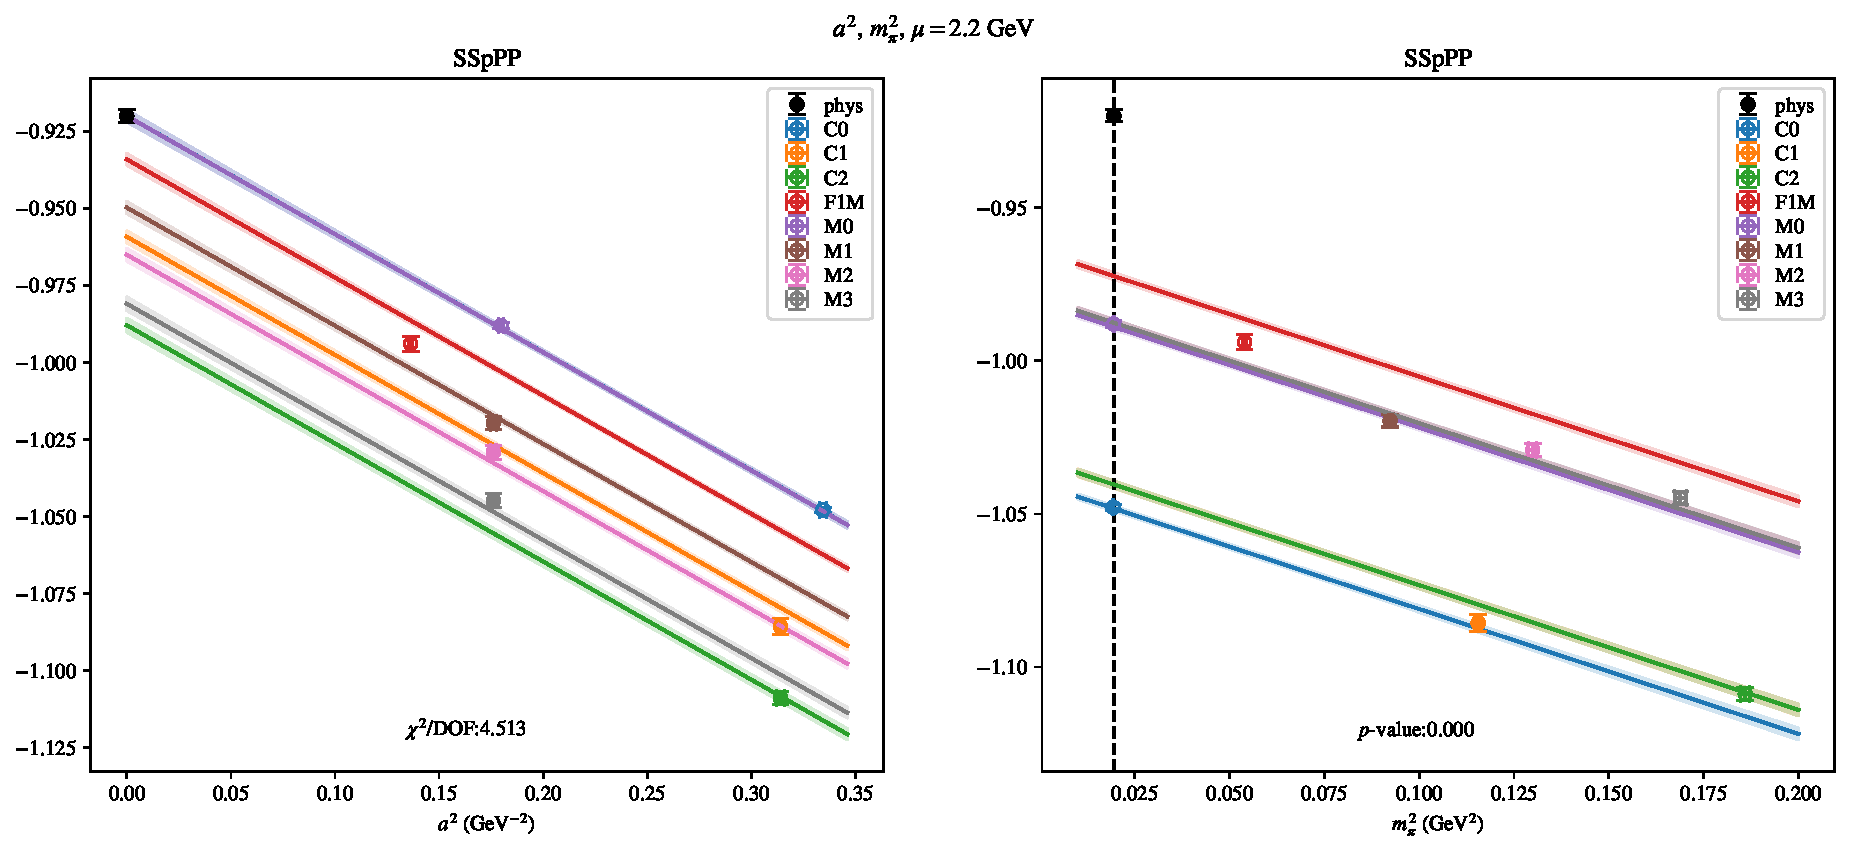
\includepdf[link, pages=-]{VVmAA/SUSY/a2m2_22.pdf}
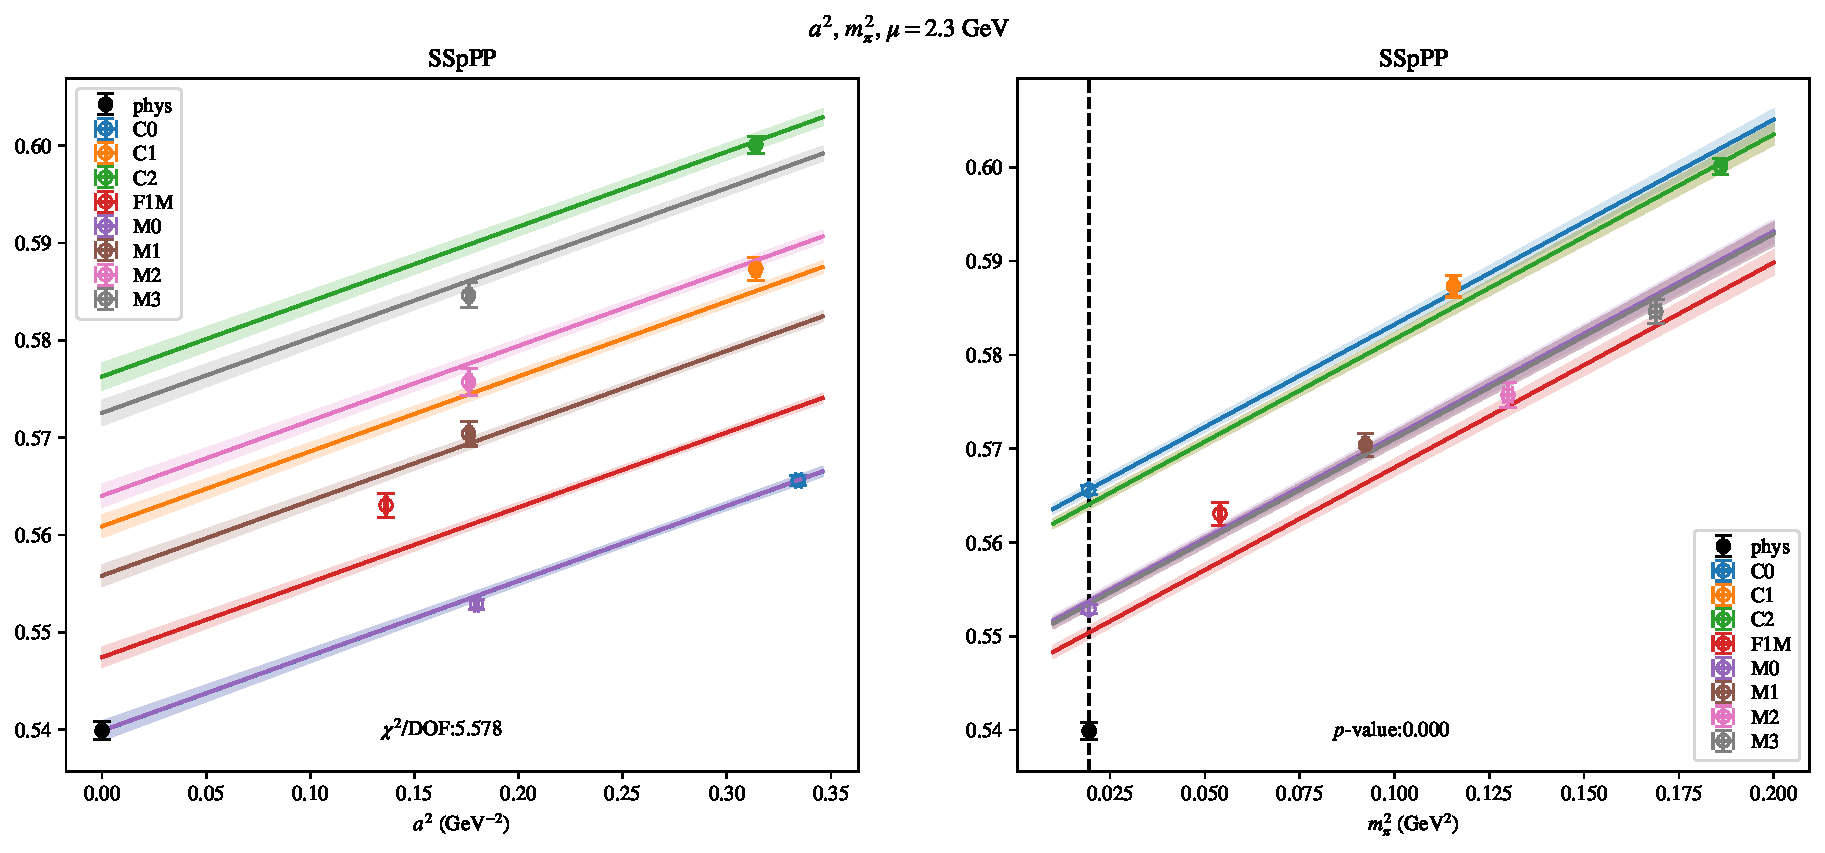
\includepdf[link, pages=-]{VVmAA/SUSY/a2m2_23.pdf}
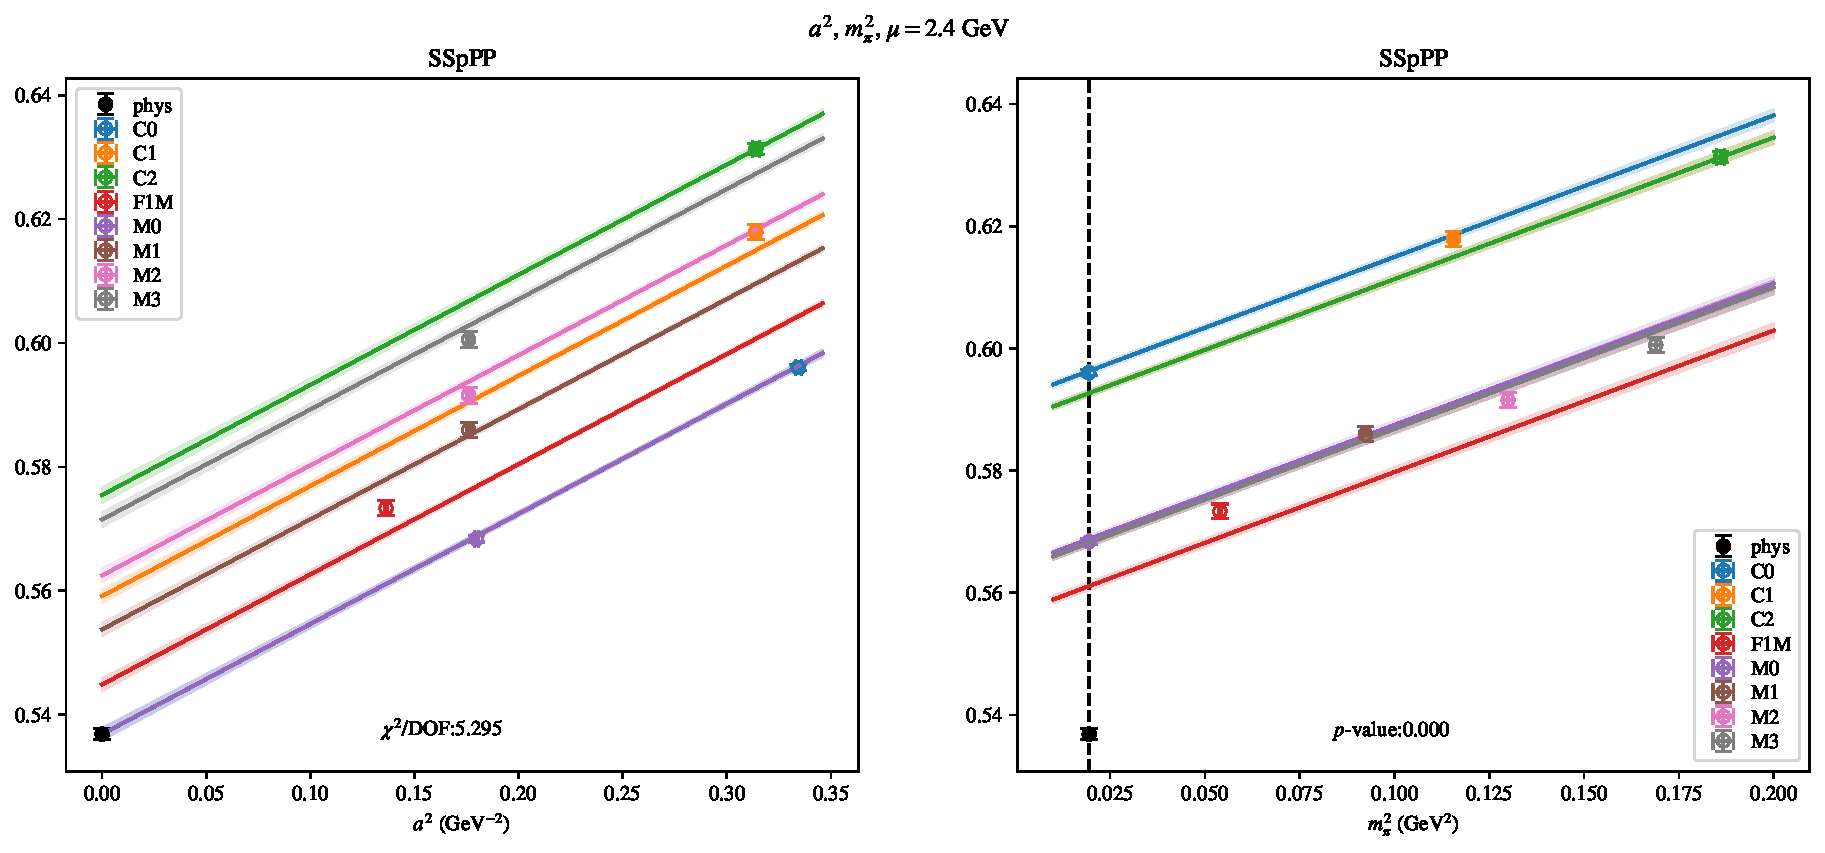
\includepdf[link, pages=-]{VVmAA/SUSY/a2m2_24.pdf}
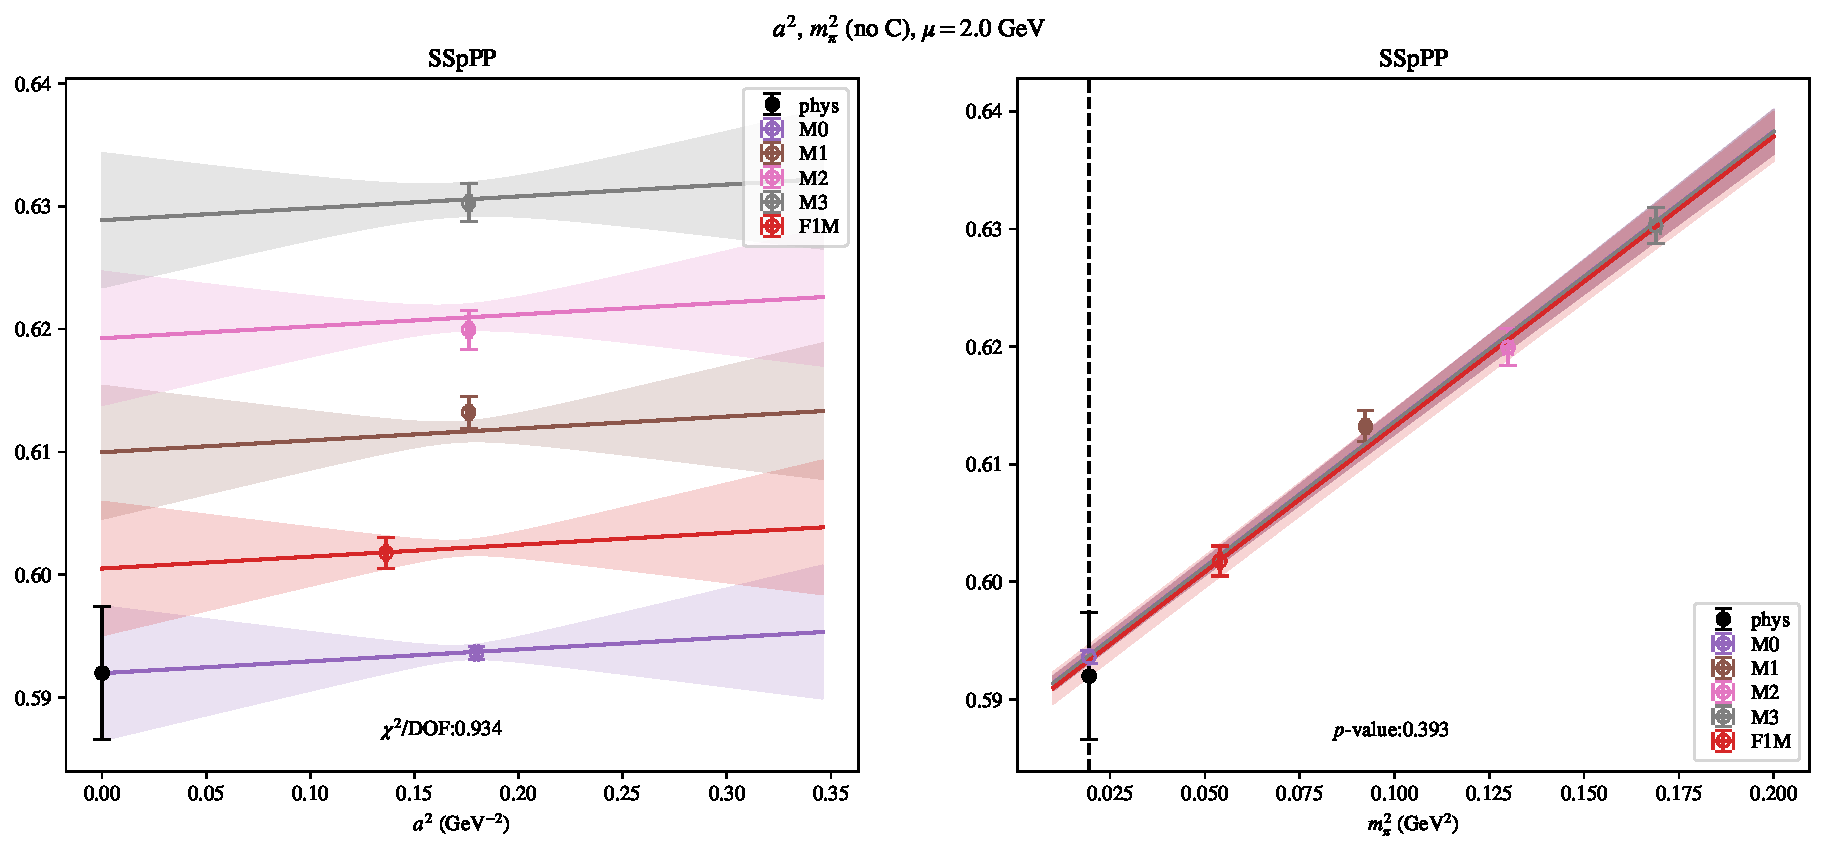
\includepdf[link, pages=-]{VVmAA/SUSY/a2m2noC_20.pdf}
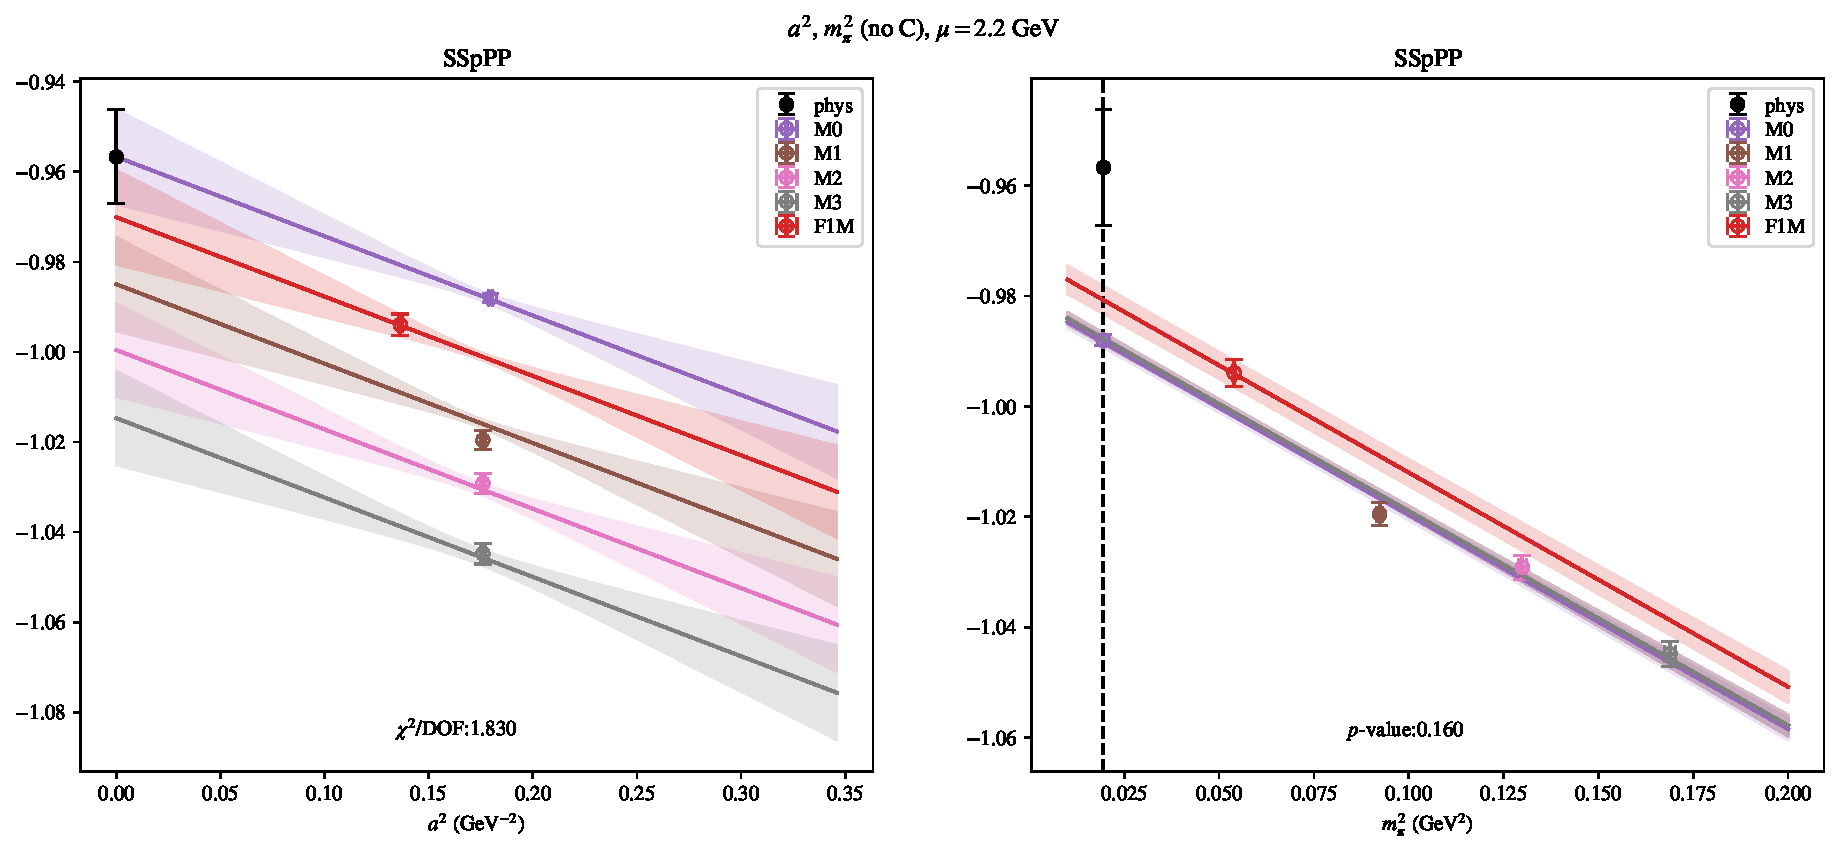
\includepdf[link, pages=-]{VVmAA/SUSY/a2m2noC_22.pdf}
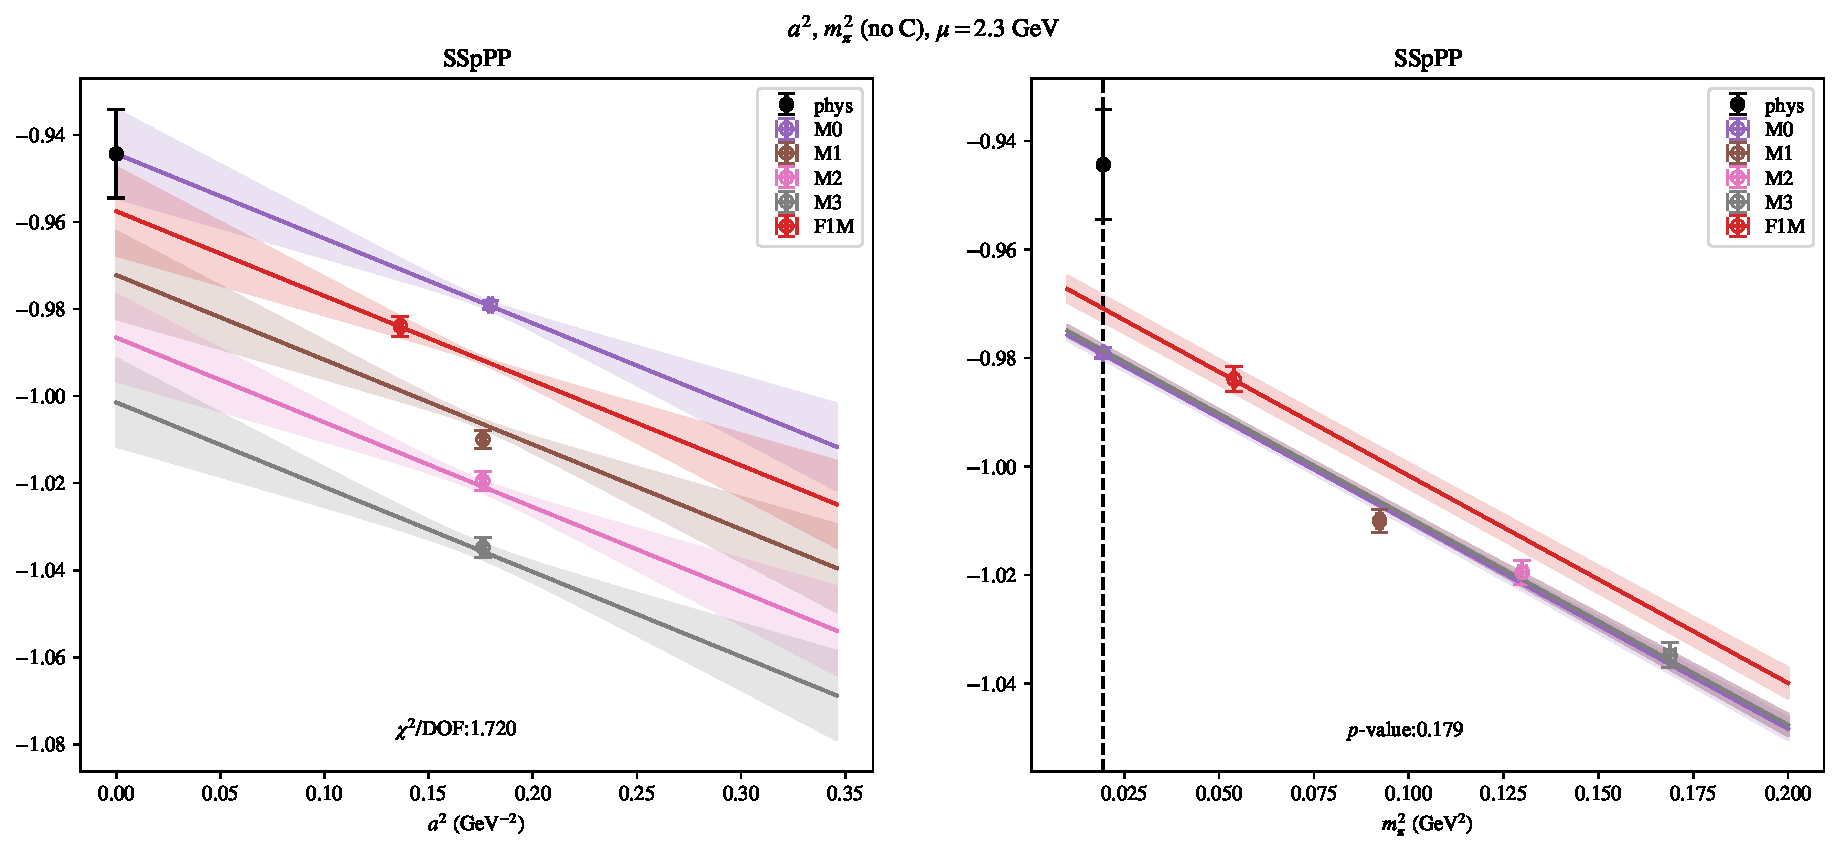
\includepdf[link, pages=-]{VVmAA/SUSY/a2m2noC_23.pdf}
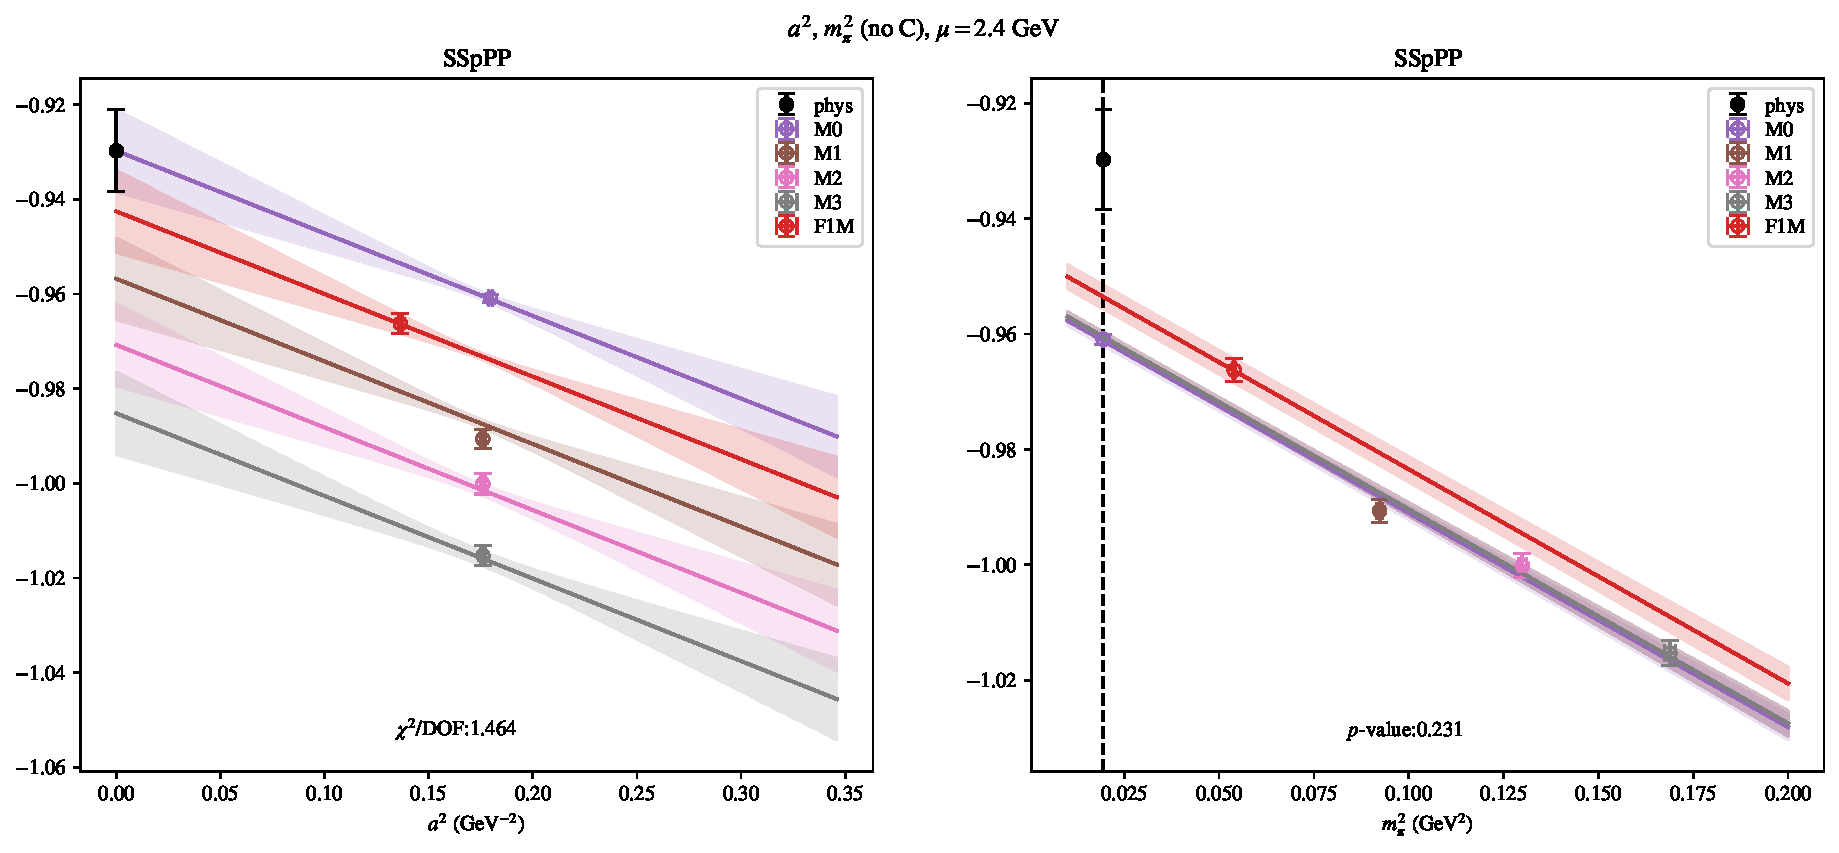
\includepdf[link, pages=-]{VVmAA/SUSY/a2m2noC_24.pdf}
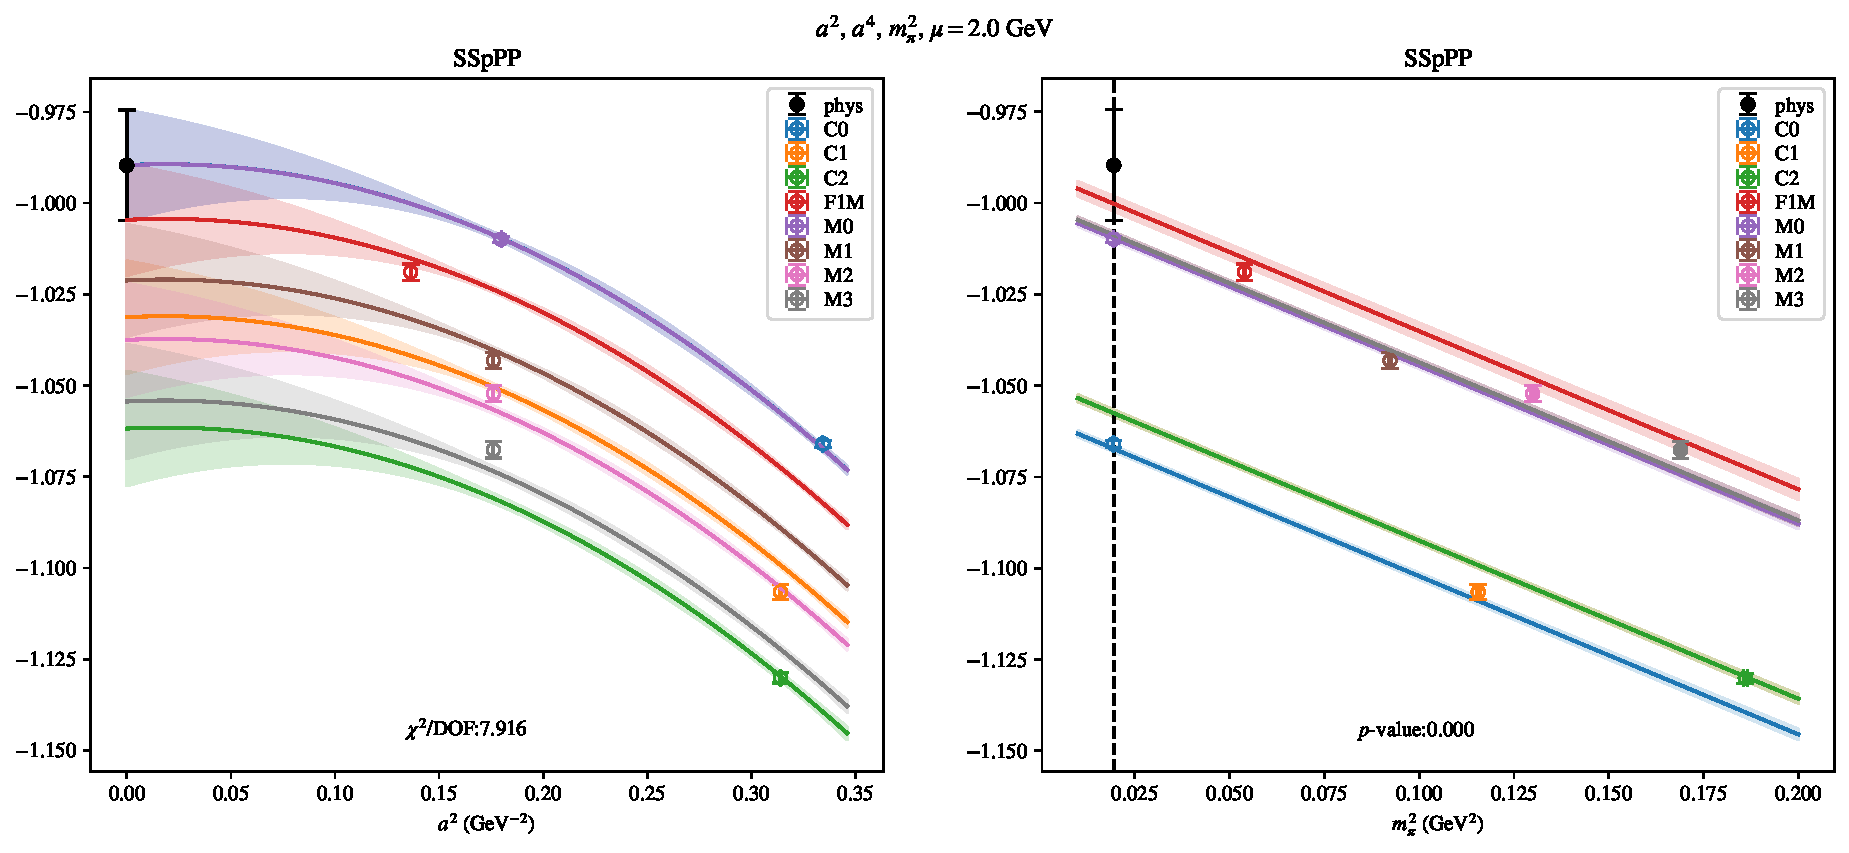
\includepdf[link, pages=-]{VVmAA/SUSY/a2a4m2_20.pdf}
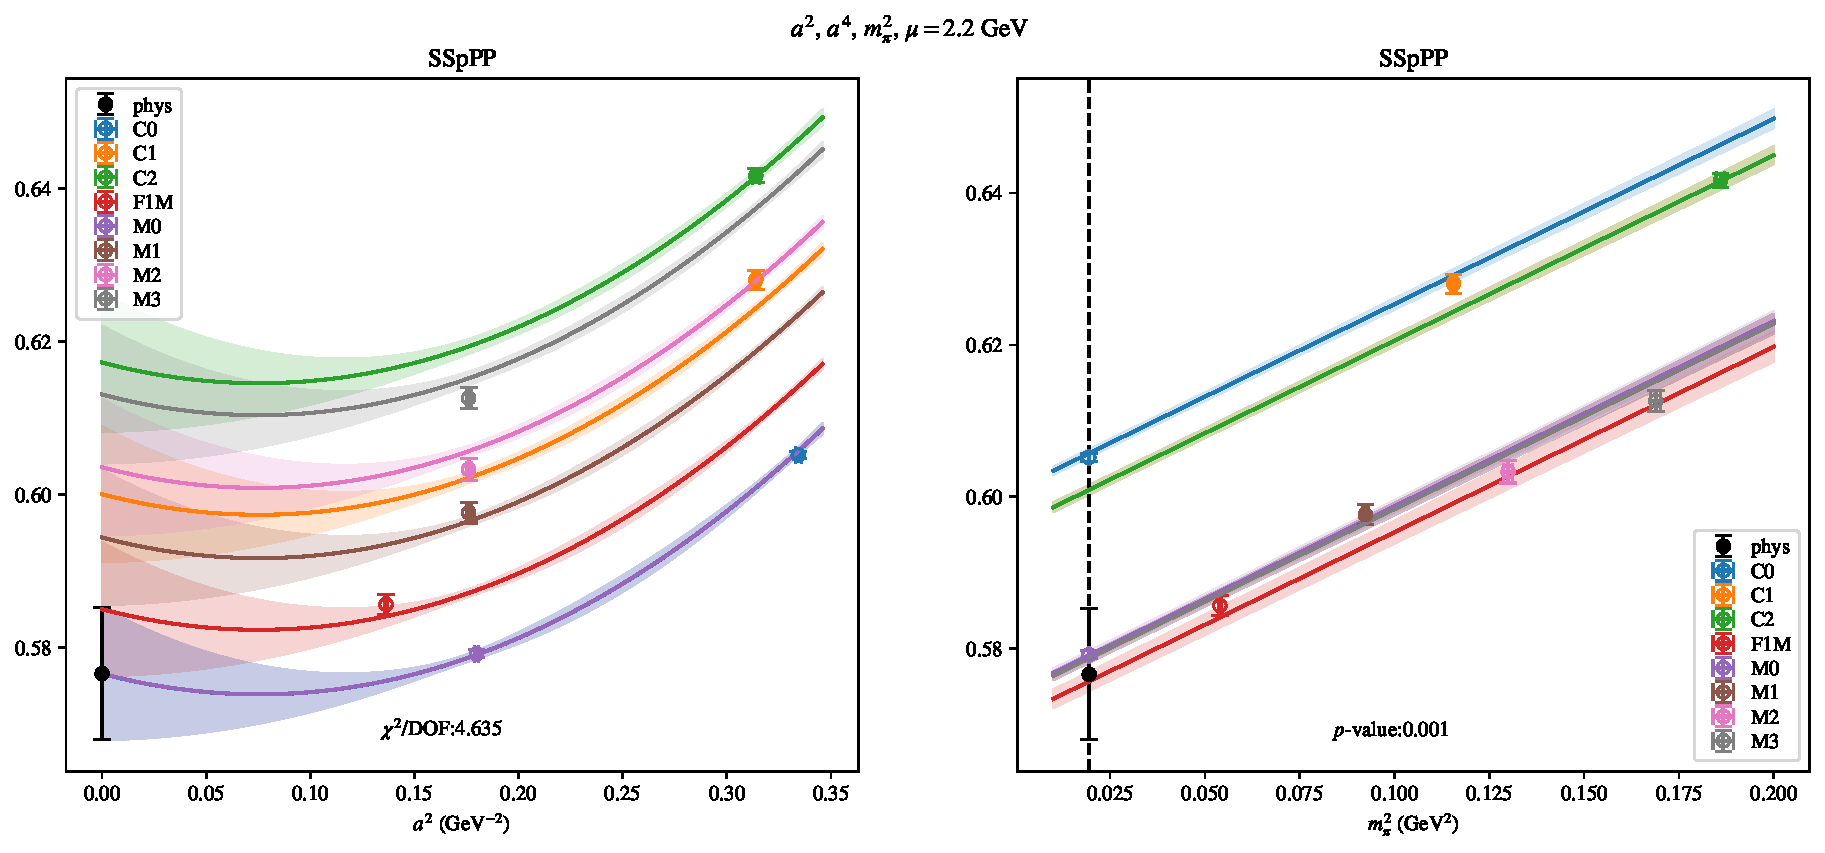
\includepdf[link, pages=-]{VVmAA/SUSY/a2a4m2_22.pdf}
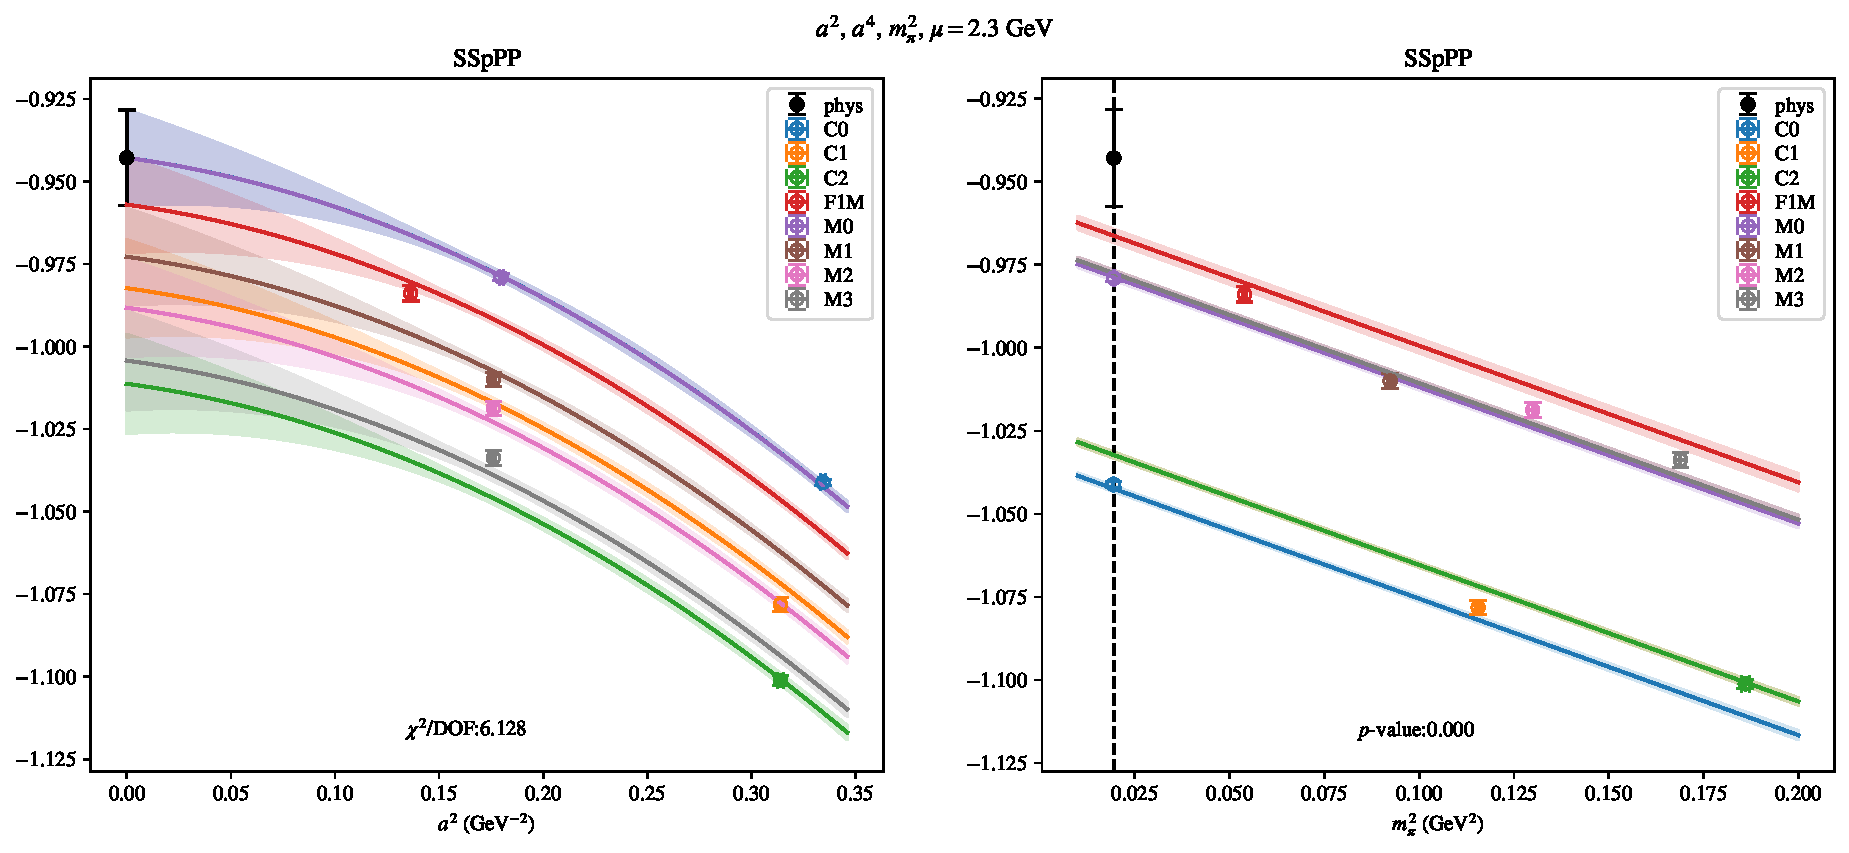
\includepdf[link, pages=-]{VVmAA/SUSY/a2a4m2_23.pdf}
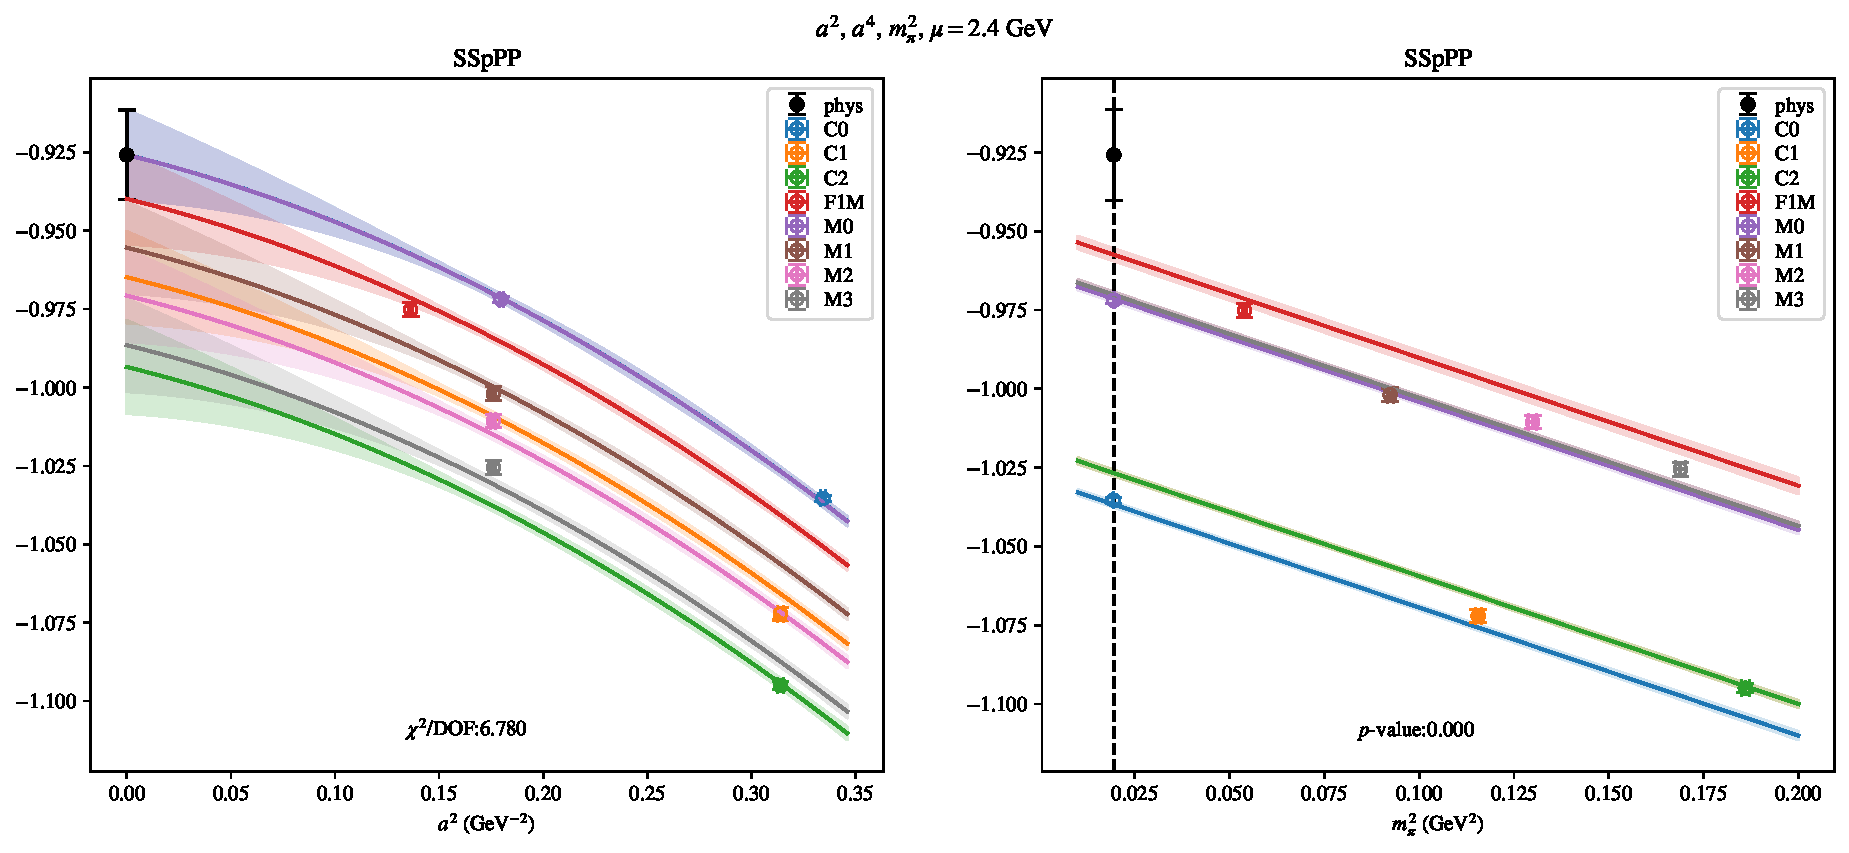
\includepdf[link, pages=-]{VVmAA/SUSY/a2a4m2_24.pdf}
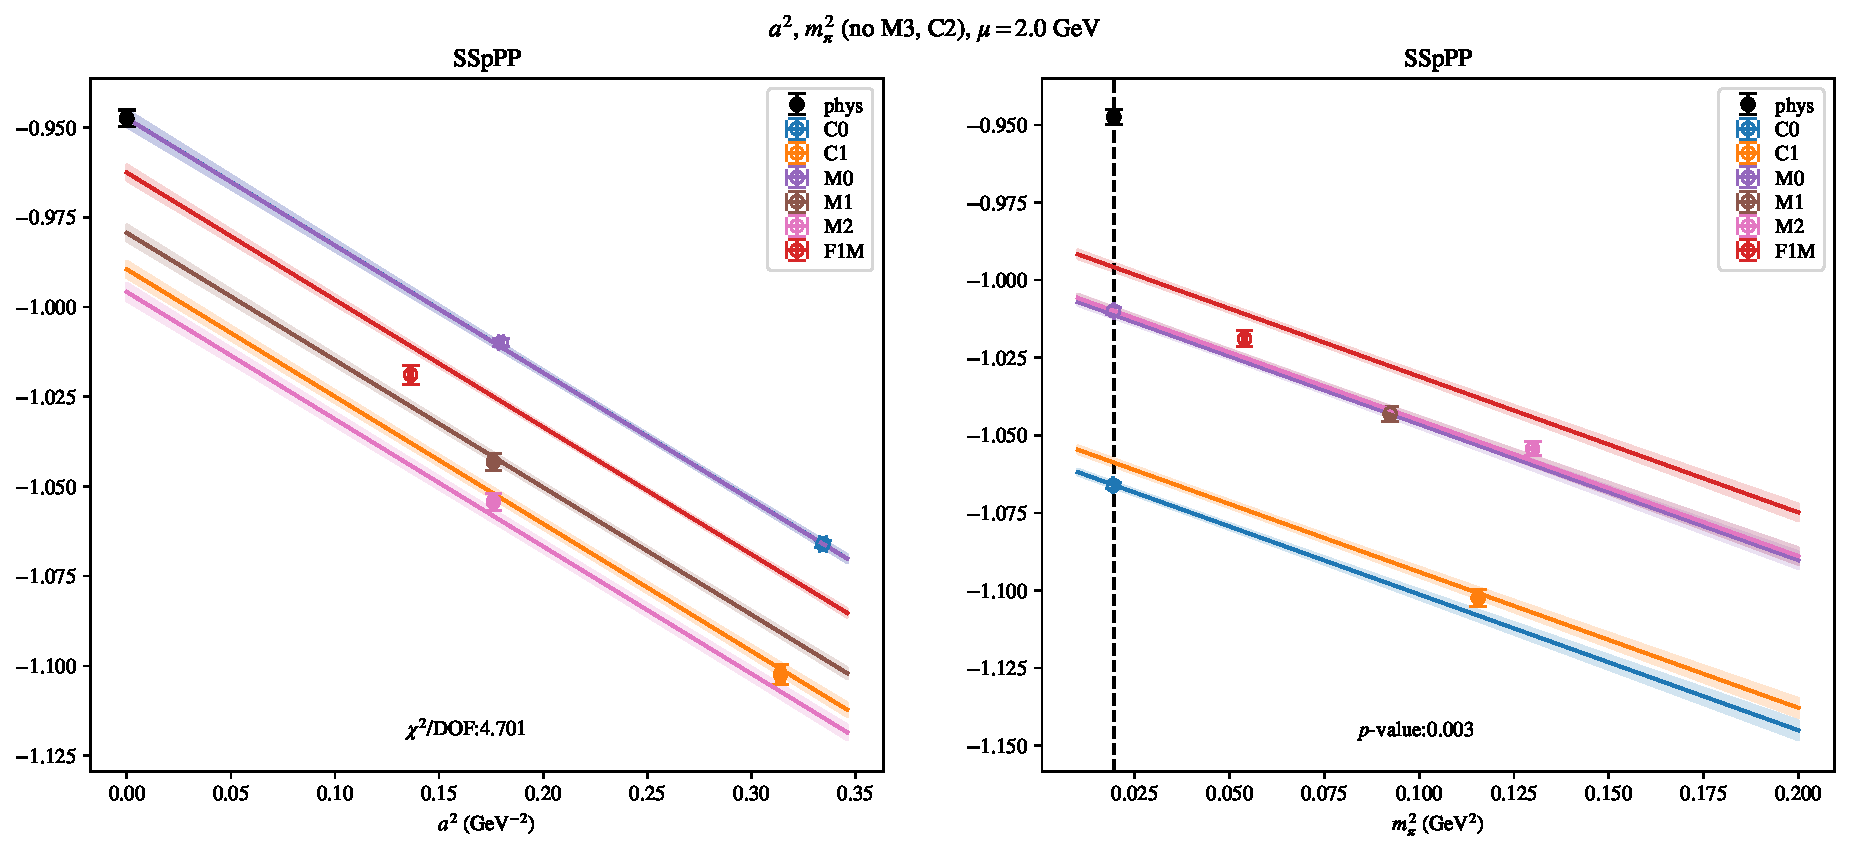
\includepdf[link, pages=-]{VVmAA/SUSY/a2m2mcut_20.pdf}
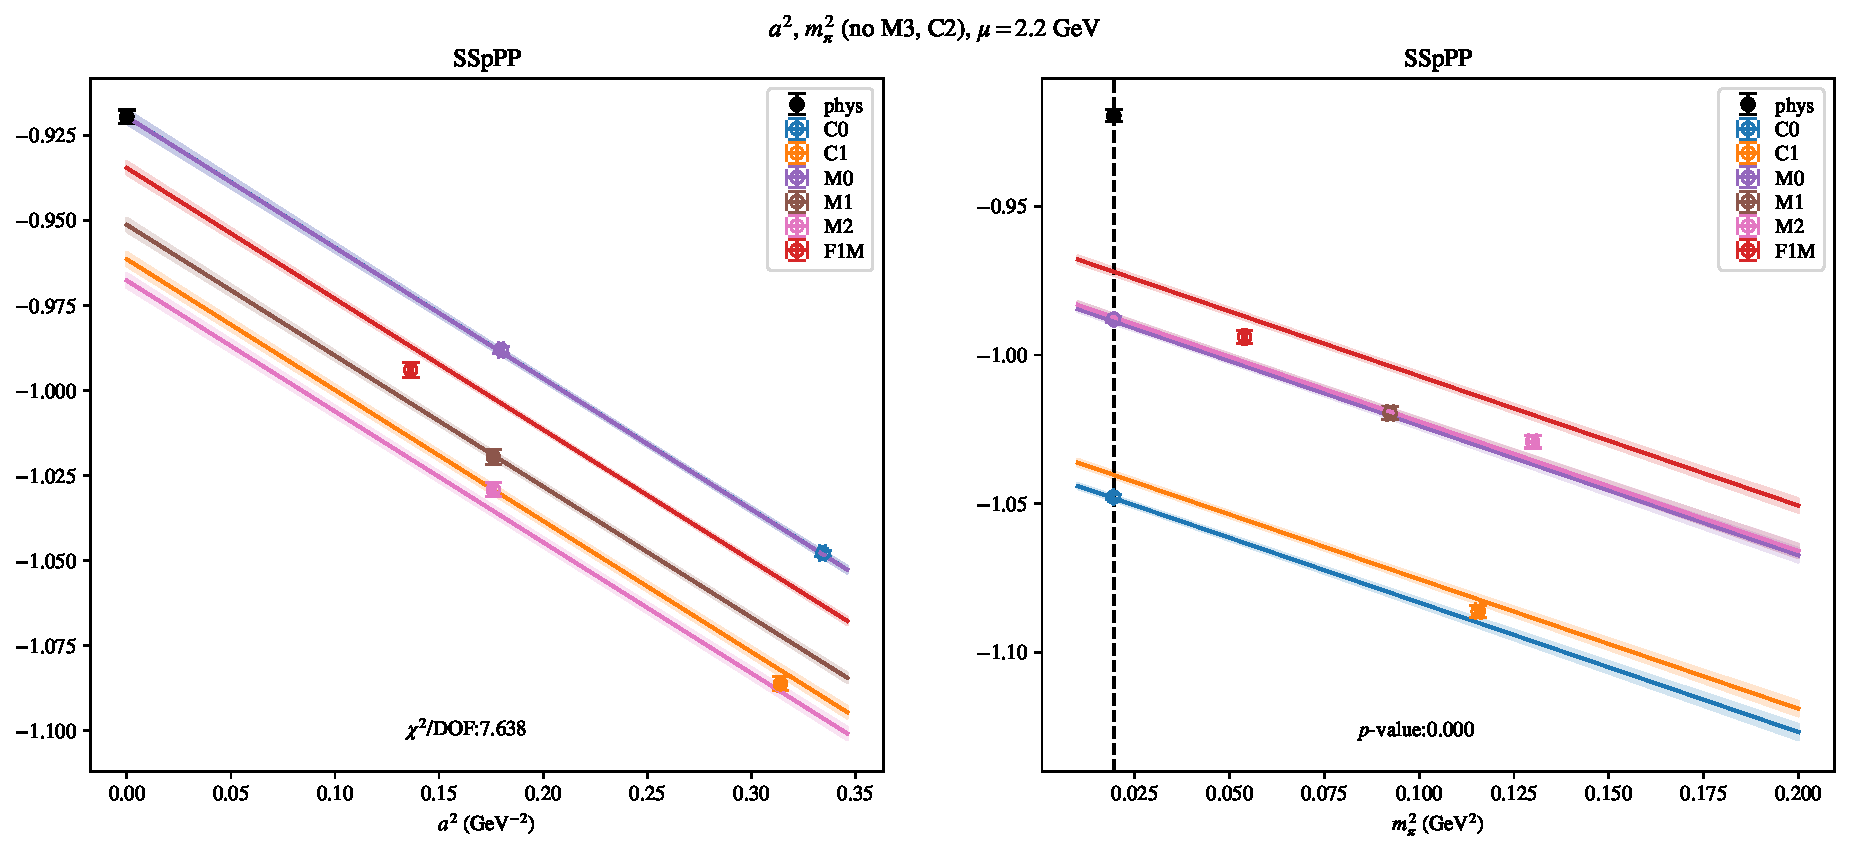
\includepdf[link, pages=-]{VVmAA/SUSY/a2m2mcut_22.pdf}
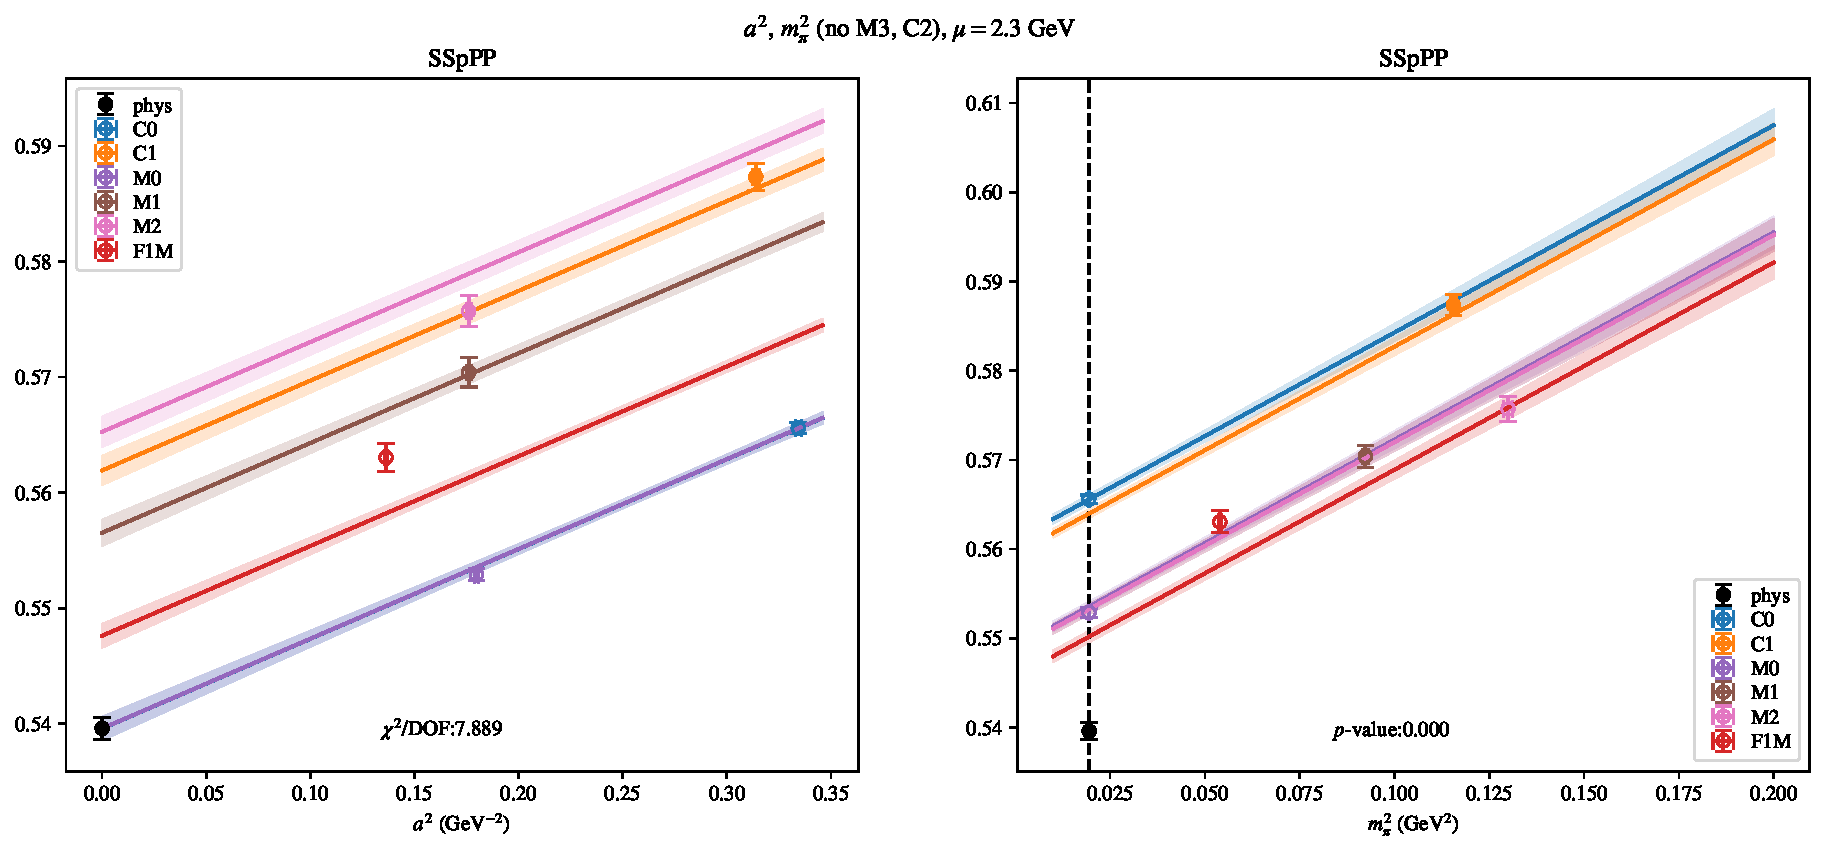
\includepdf[link, pages=-]{VVmAA/SUSY/a2m2mcut_23.pdf}
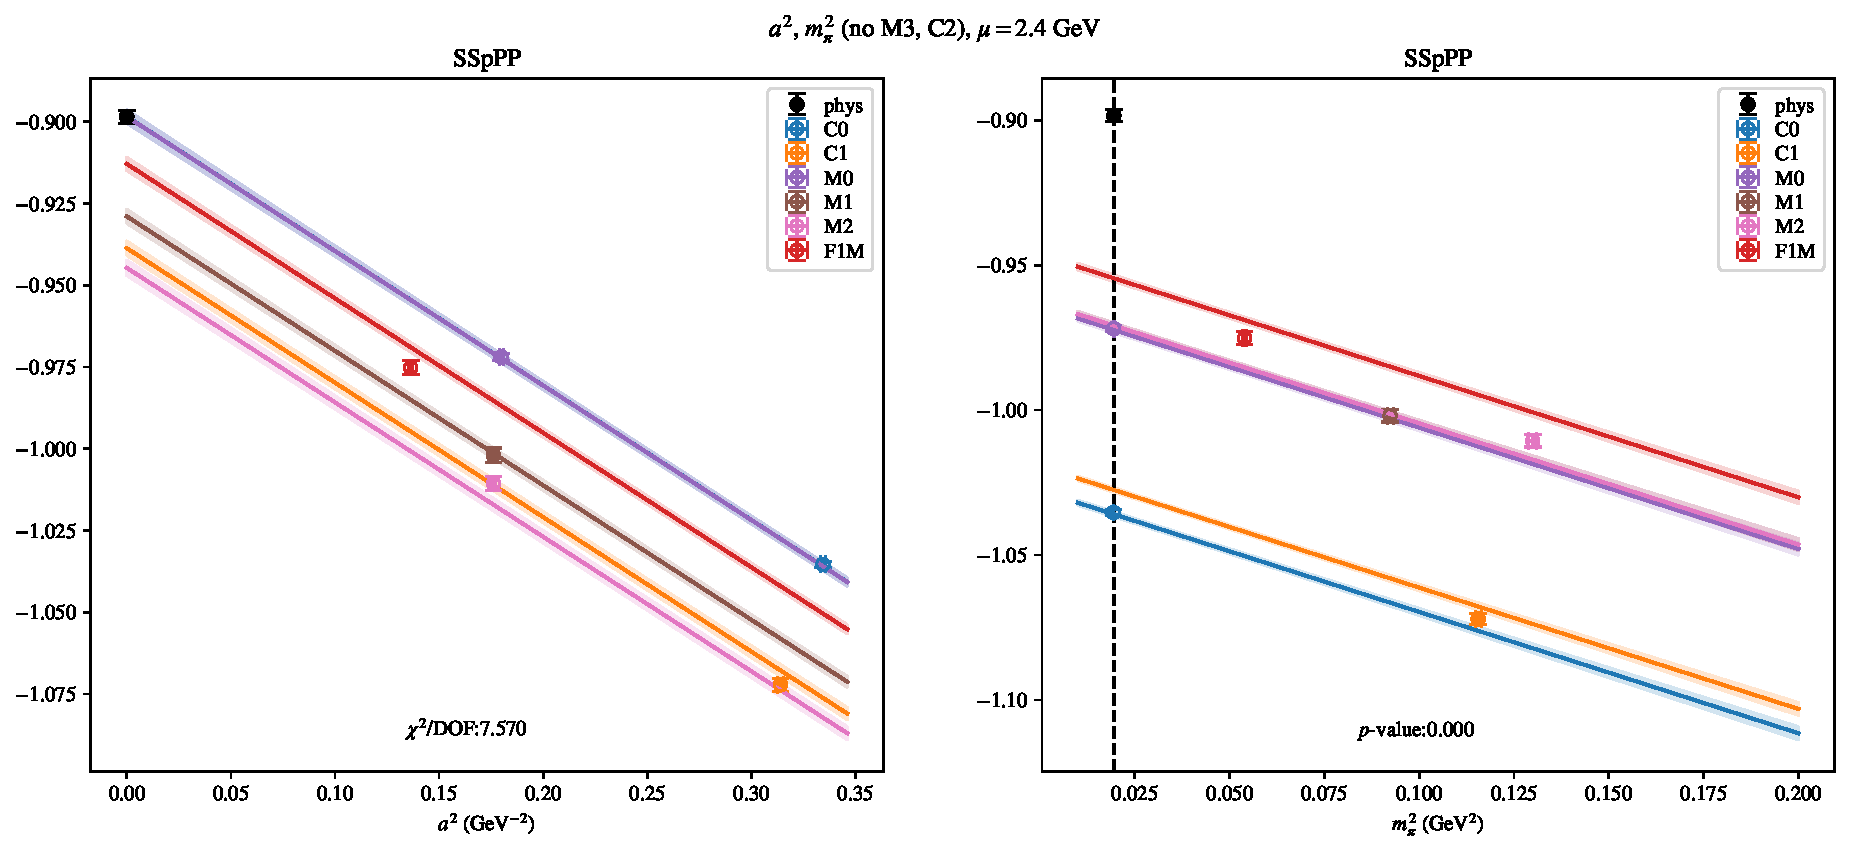
\includepdf[link, pages=-]{VVmAA/SUSY/a2m2mcut_24.pdf}
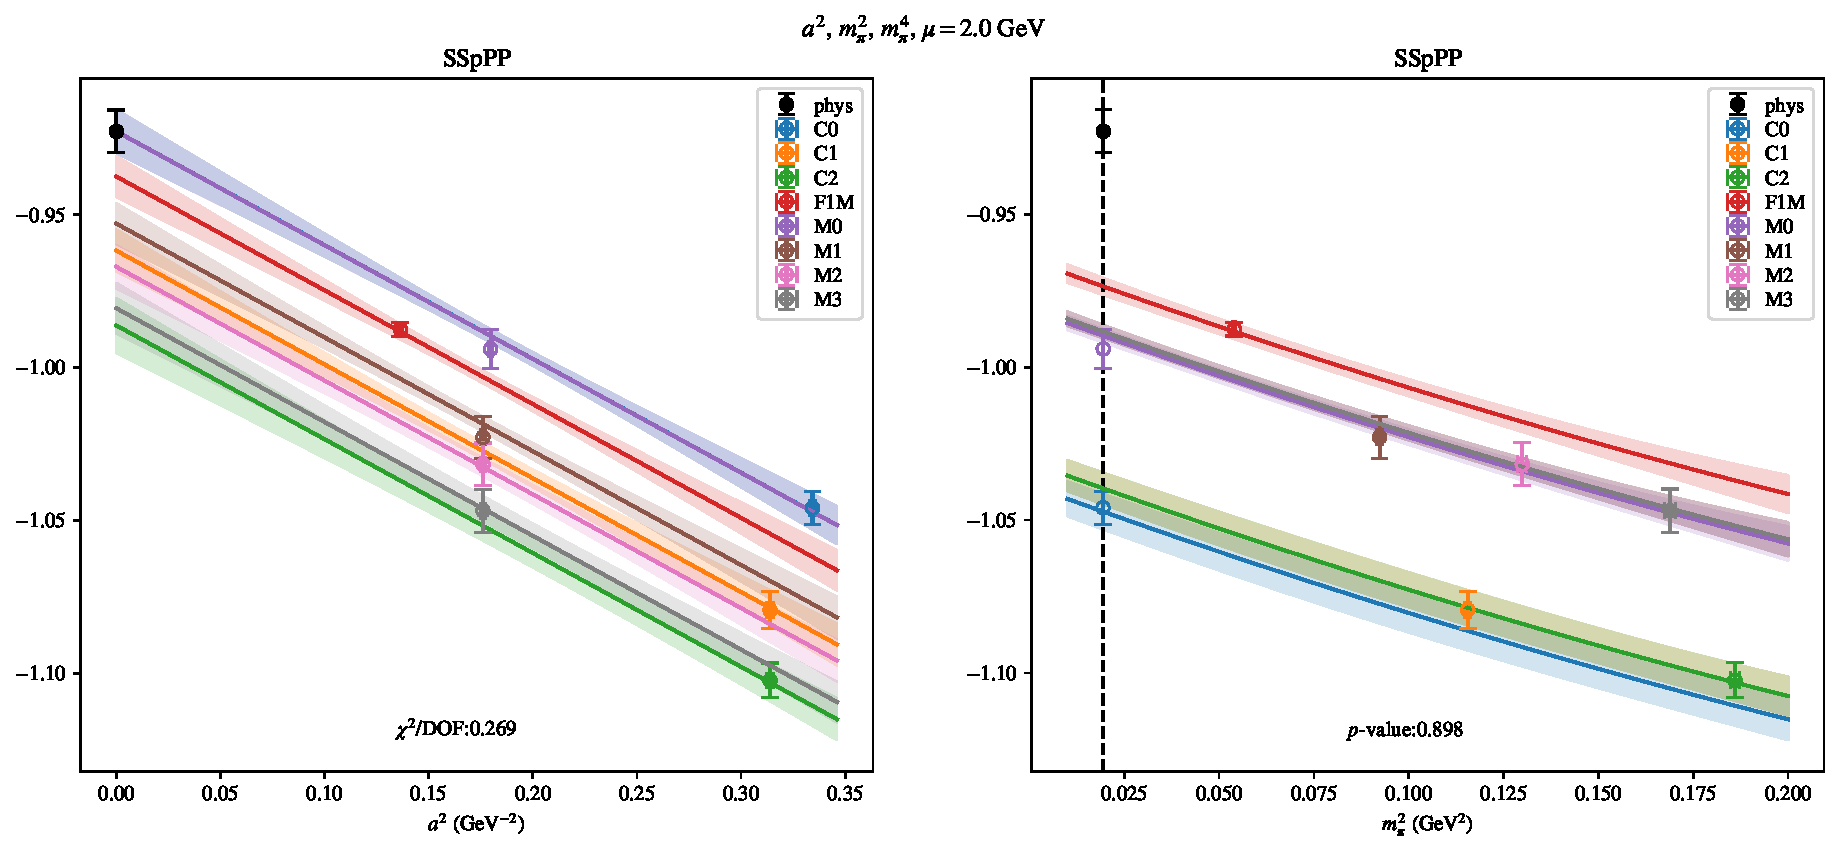
\includepdf[link, pages=-]{VVmAA/SUSY/a2m2m4_20.pdf}
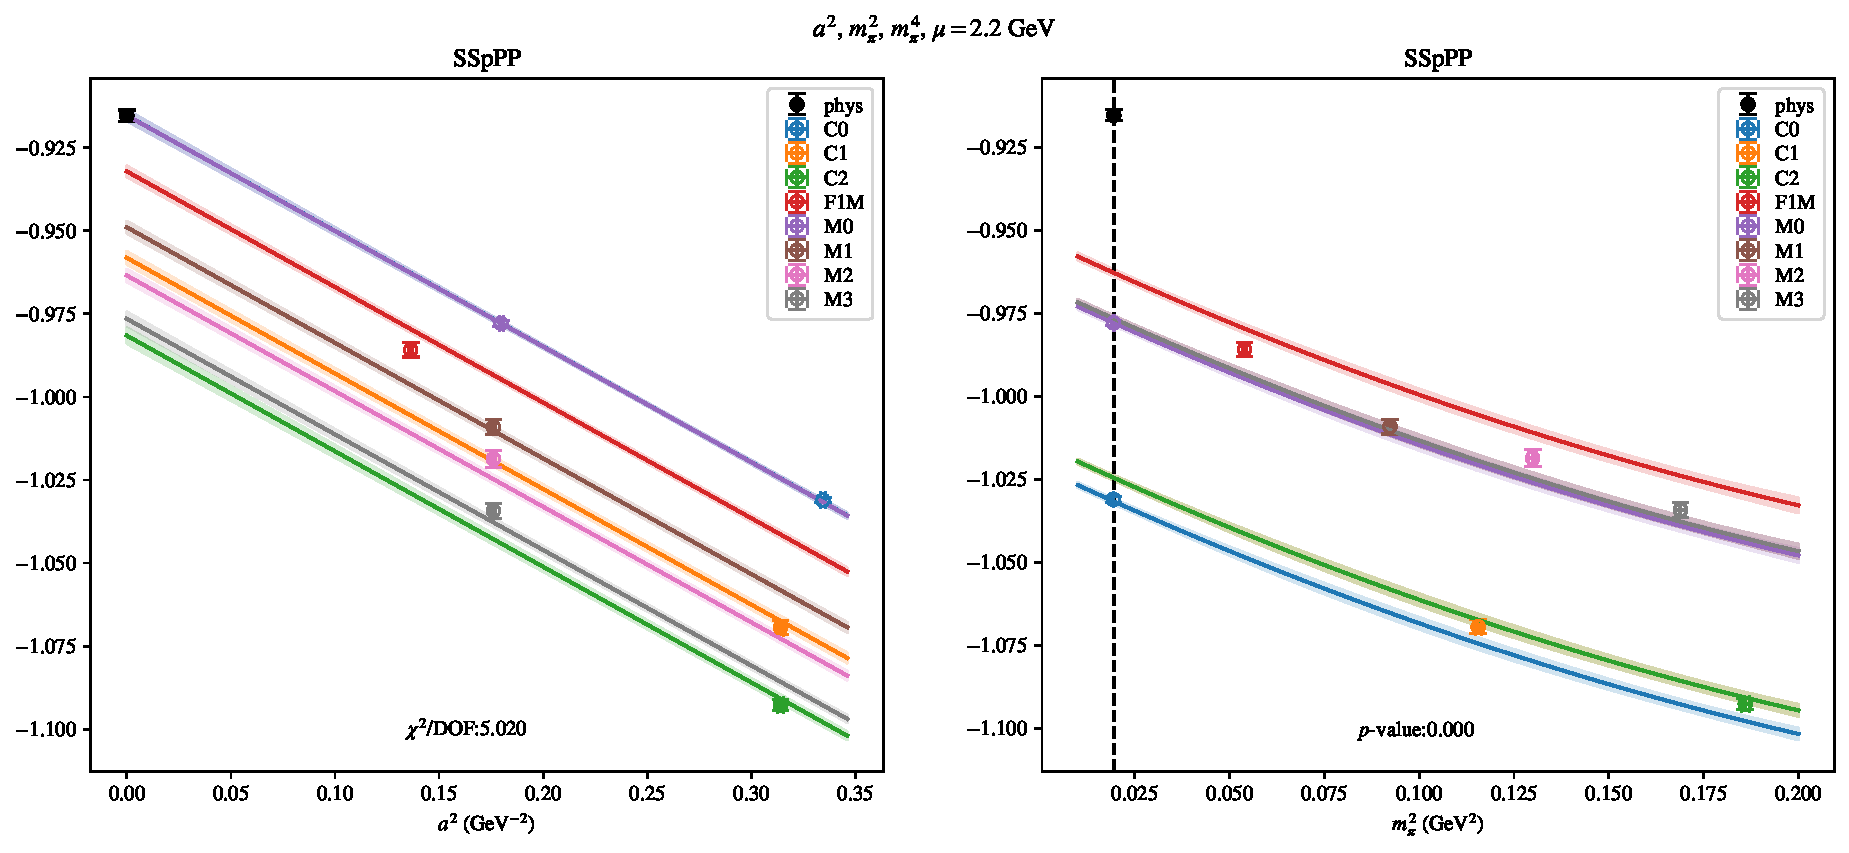
\includepdf[link, pages=-]{VVmAA/SUSY/a2m2m4_22.pdf}
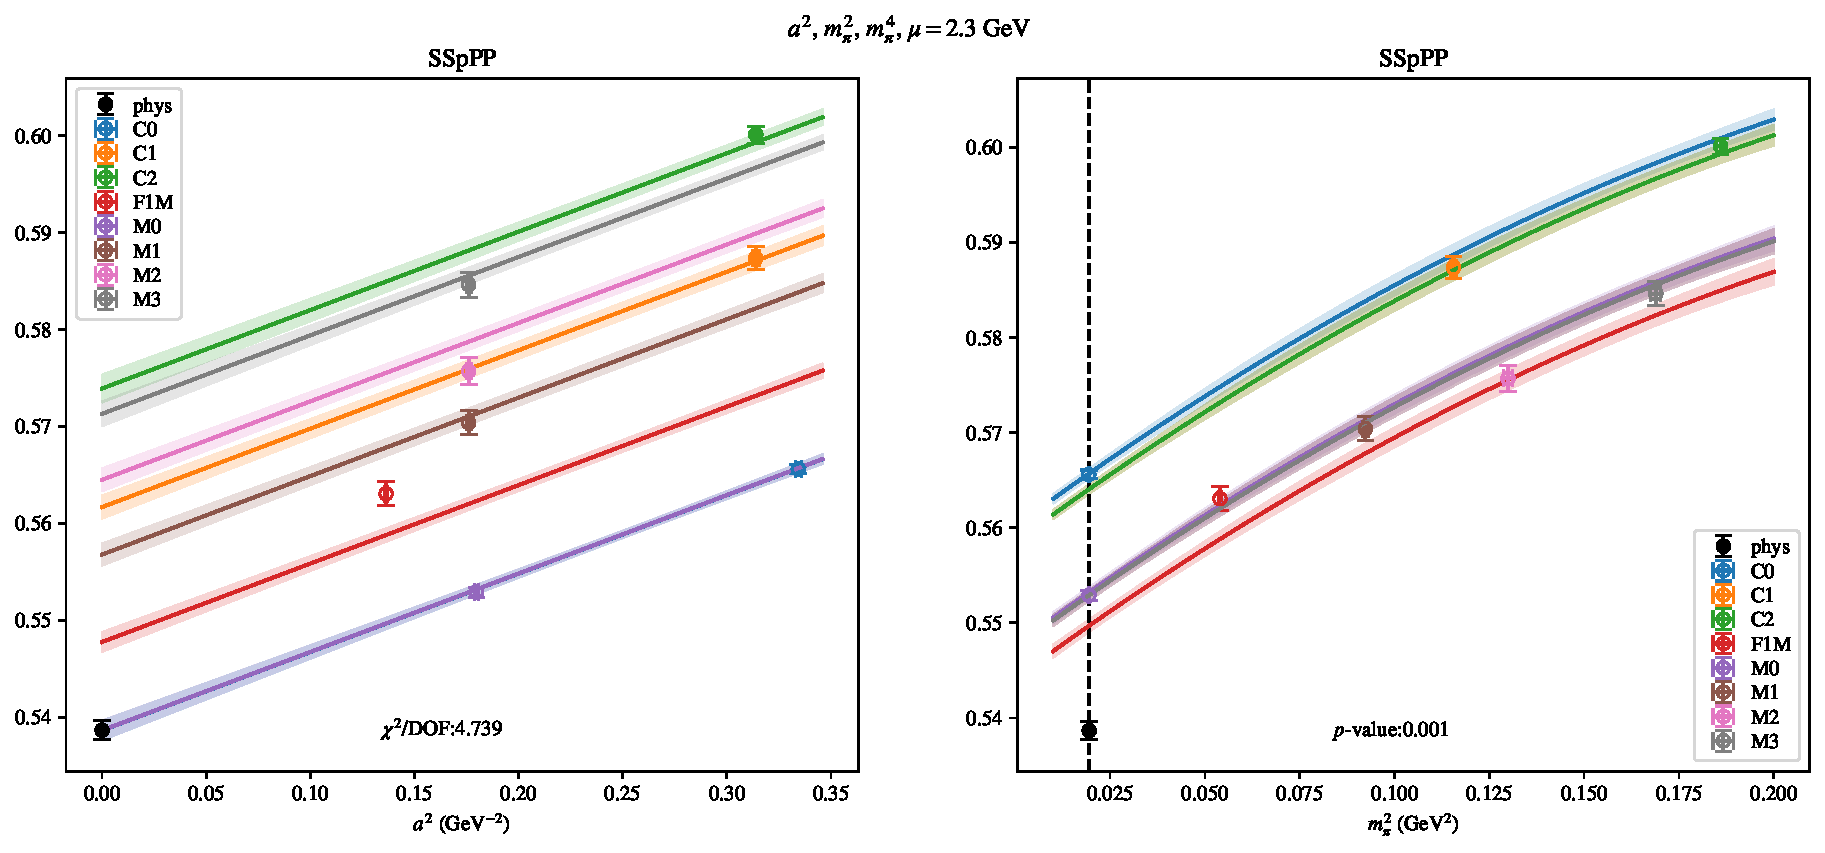
\includepdf[link, pages=-]{VVmAA/SUSY/a2m2m4_23.pdf}
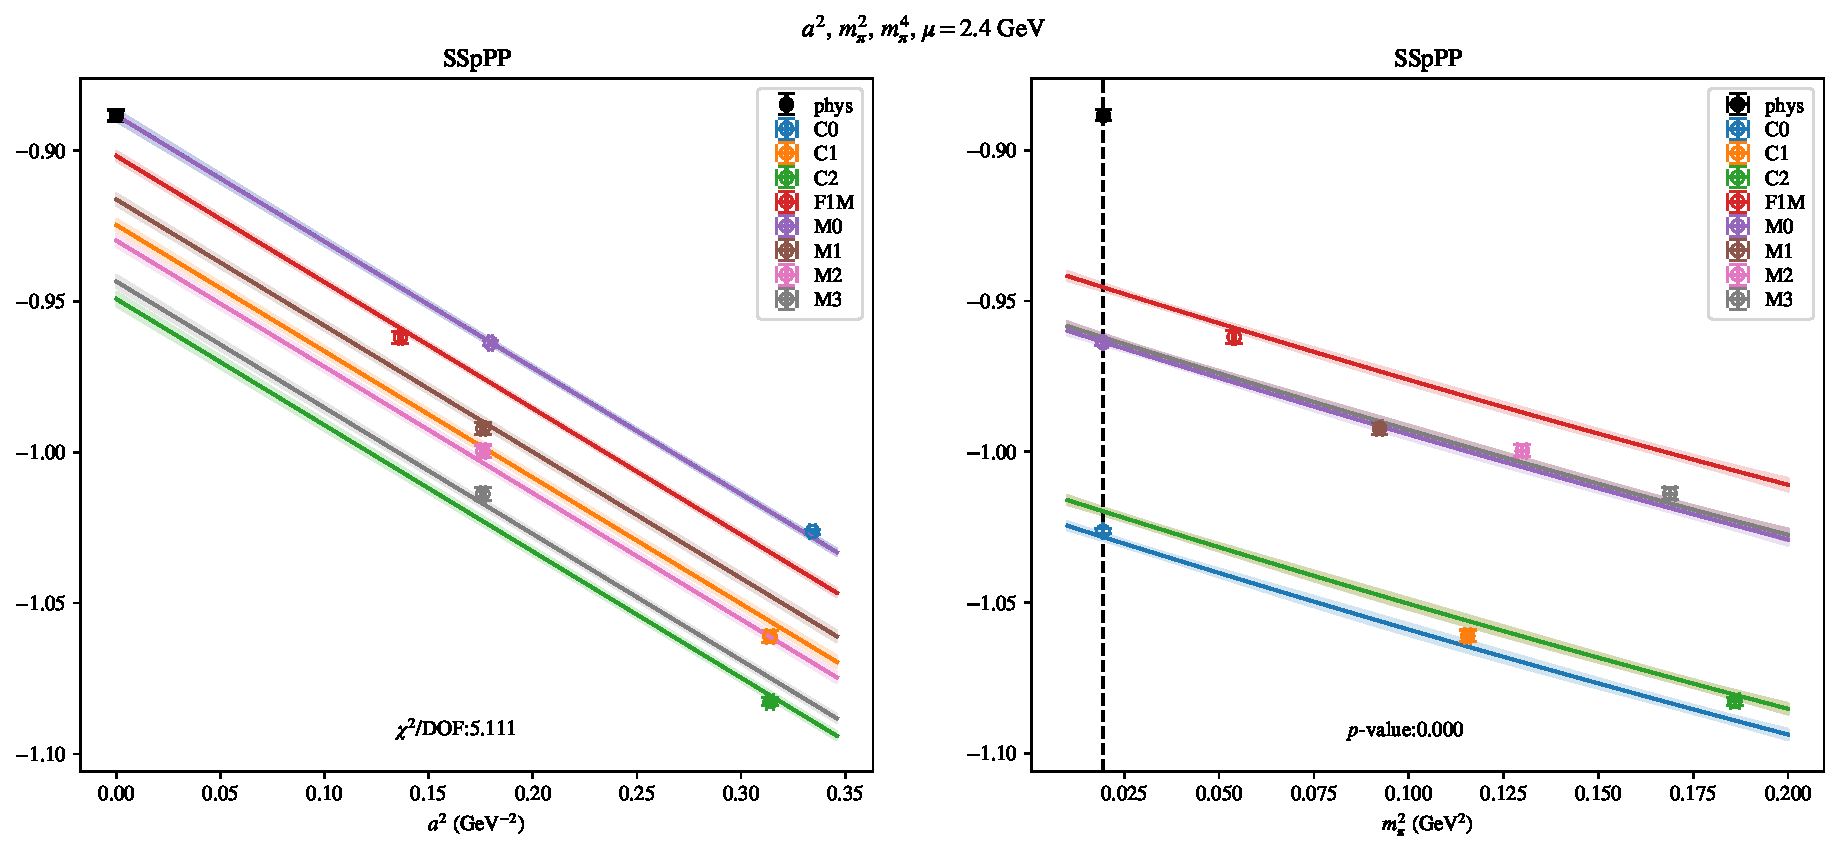
\includepdf[link, pages=-]{VVmAA/SUSY/a2m2m4_24.pdf}
\clearpage
\section{$\mathcal{B}_3$}
\begin{table}[h!]
\begin{center}
\begin{tabular}{|c|c|c|c|c|c|}
\hline
$\mu$ (GeV) & $a^2$, $m_\pi^2$& $a^2$, $m_\pi^2$ (no C)& $a^2$, $a^4$, $m_\pi^2$& $a^2$, $m_\pi^2$ (no M3, C2)& $a^2$, $m_\pi^2$, $m_\pi^4$\\
\hline
2.0& \hyperlink{SSmPP/SUSY/a2m2_20.pdf.1}{\textbf{0.28165(62)}: 4.452 (0.0)} & \hyperlink{SSmPP/SUSY/a2m2noC_20.pdf.1}{\textbf{0.2859(29)}: 4.418 (0.012)} & \hyperlink{SSmPP/SUSY/a2a4m2_20.pdf.1}{\textbf{0.2826(53)}: 5.554 (0.0)} & \hyperlink{SSmPP/SUSY/a2m2mcut_20.pdf.1}{\textbf{0.28156(69)}: 4.754 (0.003)} & \hyperlink{SSmPP/SUSY/a2m2m4_20.pdf.1}{\textbf{0.28089(69)}: 3.775 (0.005)}\\
2.2& \hyperlink{SSmPP/SUSY/a2m2_22.pdf.1}{\textbf{0.27304(61)}: 6.167 (0.0)} & \hyperlink{SSmPP/SUSY/a2m2noC_22.pdf.1}{\textbf{0.2789(28)}: 3.601 (0.027)} & \hyperlink{SSmPP/SUSY/a2a4m2_22.pdf.1}{\textbf{0.2744(52)}: 7.685 (0.0)} & \hyperlink{SSmPP/SUSY/a2m2mcut_22.pdf.1}{\textbf{0.27326(69)}: 5.682 (0.001)} & \hyperlink{SSmPP/SUSY/a2m2m4_22.pdf.1}{\textbf{0.27235(68)}: 5.967 (0.0)}\\
2.3& \hyperlink{SSmPP/SUSY/a2m2_23.pdf.1}{\textbf{0.26919(61)}: 6.876 (0.0)} & \hyperlink{SSmPP/SUSY/a2m2noC_23.pdf.1}{\textbf{0.2760(28)}: 3.885 (0.021)} & \hyperlink{SSmPP/SUSY/a2a4m2_23.pdf.1}{\textbf{0.2718(52)}: 8.503 (0.0)} & \hyperlink{SSmPP/SUSY/a2m2mcut_23.pdf.1}{\textbf{0.26941(69)}: 6.832 (0.0)} & \hyperlink{SSmPP/SUSY/a2m2m4_23.pdf.1}{\textbf{0.26850(69)}: 6.786 (0.0)}\\
2.4& \hyperlink{SSmPP/SUSY/a2m2_24.pdf.1}{\textbf{0.26581(62)}: 7.684 (0.0)} & \hyperlink{SSmPP/SUSY/a2m2noC_24.pdf.1}{\textbf{0.2728(27)}: 3.894 (0.02)} & \hyperlink{SSmPP/SUSY/a2a4m2_24.pdf.1}{\textbf{0.2681(52)}: 9.534 (0.0)} & \hyperlink{SSmPP/SUSY/a2m2mcut_24.pdf.1}{\textbf{0.26611(70)}: 7.989 (0.0)} & \hyperlink{SSmPP/SUSY/a2m2m4_24.pdf.1}{\textbf{0.26517(70)}: 8.018 (0.0)}\\
\hline
\end{tabular}
\caption{Physical point value from chiral and continuum extrapolation at renormalisation scale $\mu$. Entries are \textbf{value(error)}: $\chi^2/\text{DOF}$ ($p$-value).}
\end{center}
\end{table}
\begin{table}[h!]
\begin{center}
\begin{tabular}{|c c|c|c|c|c|c|}
\hline
$\mu$ (GeV) &  & $a^2$, $m_\pi^2$& $a^2$, $m_\pi^2$ (no C)& $a^2$, $a^4$, $m_\pi^2$& $a^2$, $m_\pi^2$ (no M3, C2)& $a^2$, $m_\pi^2$, $m_\pi^4$\\
\hline
\multirow{2}{0.5in}{2.0} & $\alpha$ & 0.642(10)& 0.550(66)& 0.60(18)& 0.642(11)& 0.652(11)\\
 & $\beta$ & 0.00695(19)& 0.00630(32)& 0.00693(20)& 0.00752(32)& 0.00952(96)\\
\hline
\multirow{2}{0.5in}{2.2} & $\alpha$ & 0.754(11)& 0.624(66)& 0.70(18)& 0.749(12)& 0.764(11)\\
 & $\beta$ & 0.00749(19)& 0.00660(27)& 0.00747(21)& 0.00809(32)& 0.00992(93)\\
\hline
\multirow{2}{0.5in}{2.3} & $\alpha$ & 0.810(11)& 0.656(66)& 0.71(19)& 0.805(12)& 0.821(12)\\
 & $\beta$ & 0.00766(19)& 0.00672(26)& 0.00762(21)& 0.00821(32)& 0.01008(94)\\
\hline
\multirow{2}{0.5in}{2.4} & $\alpha$ & 0.862(11)& 0.701(67)& 0.77(19)& 0.856(13)& 0.872(13)\\
 & $\beta$ & 0.00785(20)& 0.00682(26)& 0.00781(22)& 0.00832(32)& 0.01009(95)\\
\hline
\end{tabular}
\caption{Fit values of coefficients in $Q = Q_{phys} + \mathbf{\alpha} a^2 + \mathbf{\beta}\left(\frac{m_\pi^2}{f_\pi^2}-\frac{m_{\pi,PDG}^2}{f_\pi^2}\right) + \ldots$.}
\end{center}
\end{table}
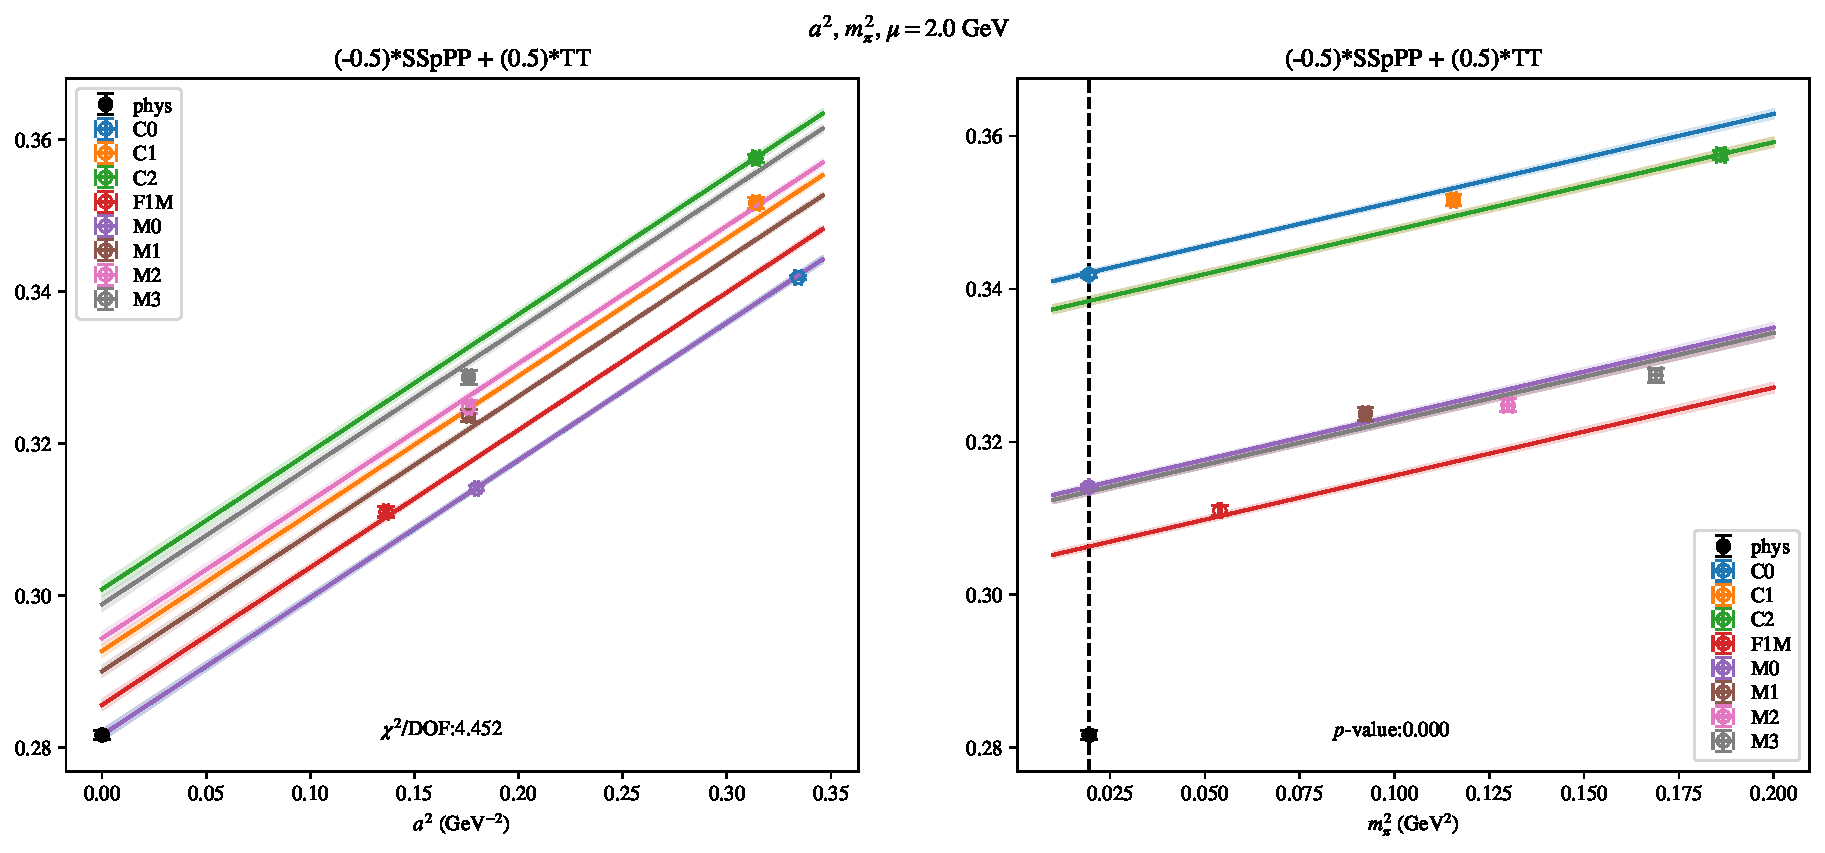
\includepdf[link, pages=-]{SSmPP/SUSY/a2m2_20.pdf}
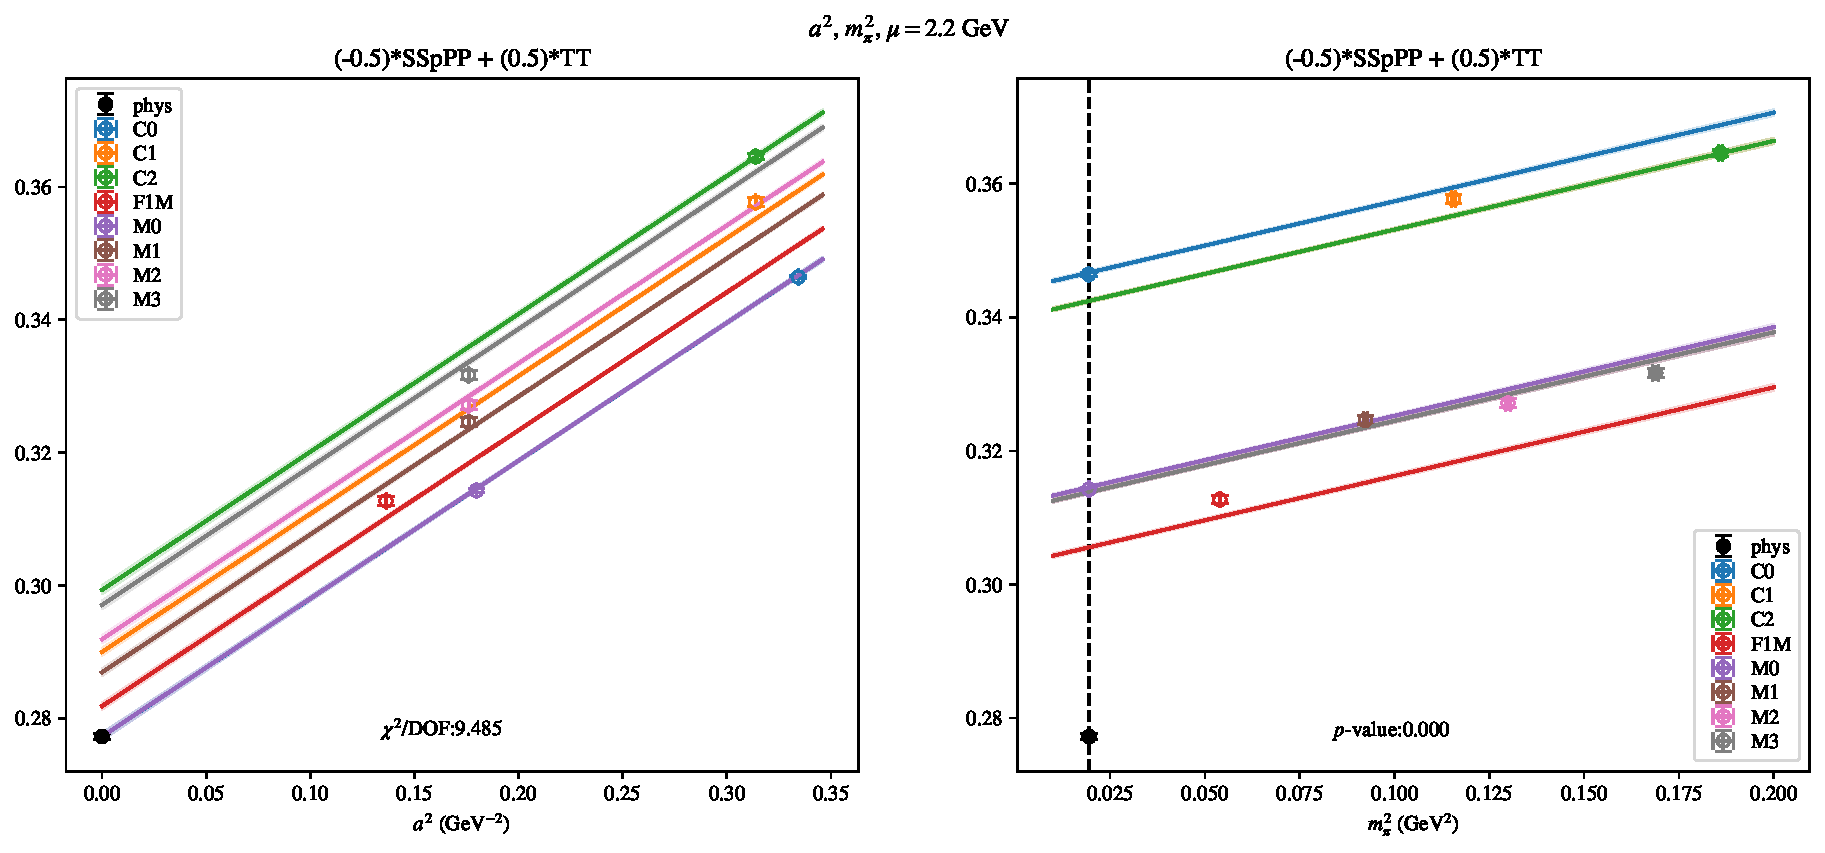
\includepdf[link, pages=-]{SSmPP/SUSY/a2m2_22.pdf}
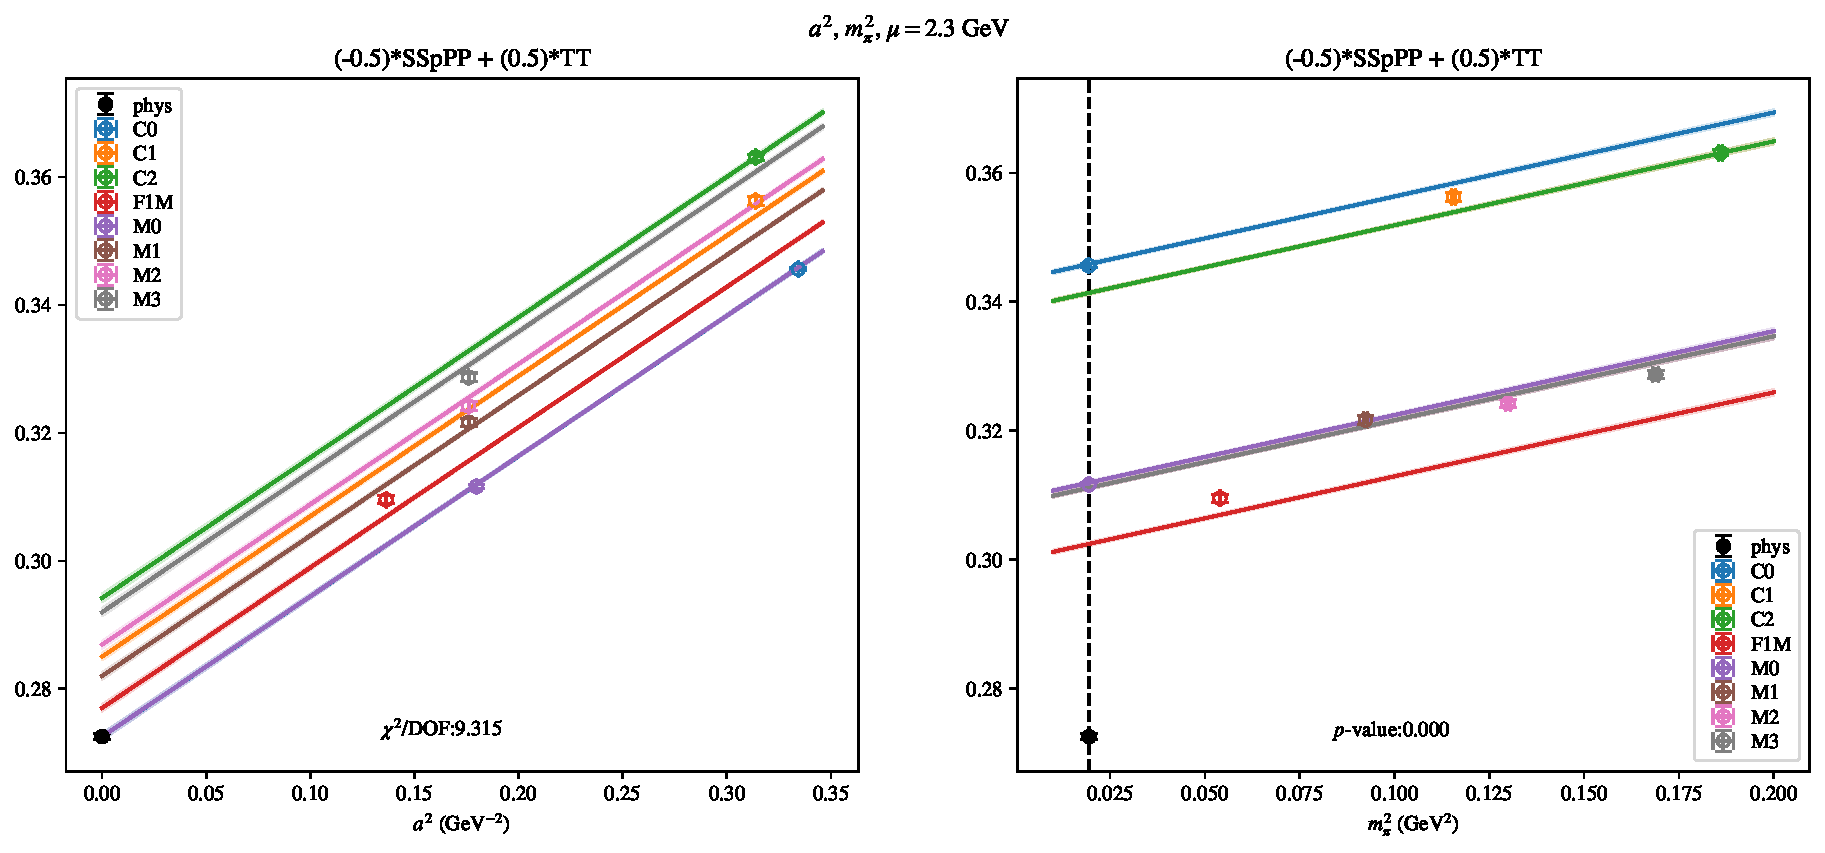
\includepdf[link, pages=-]{SSmPP/SUSY/a2m2_23.pdf}
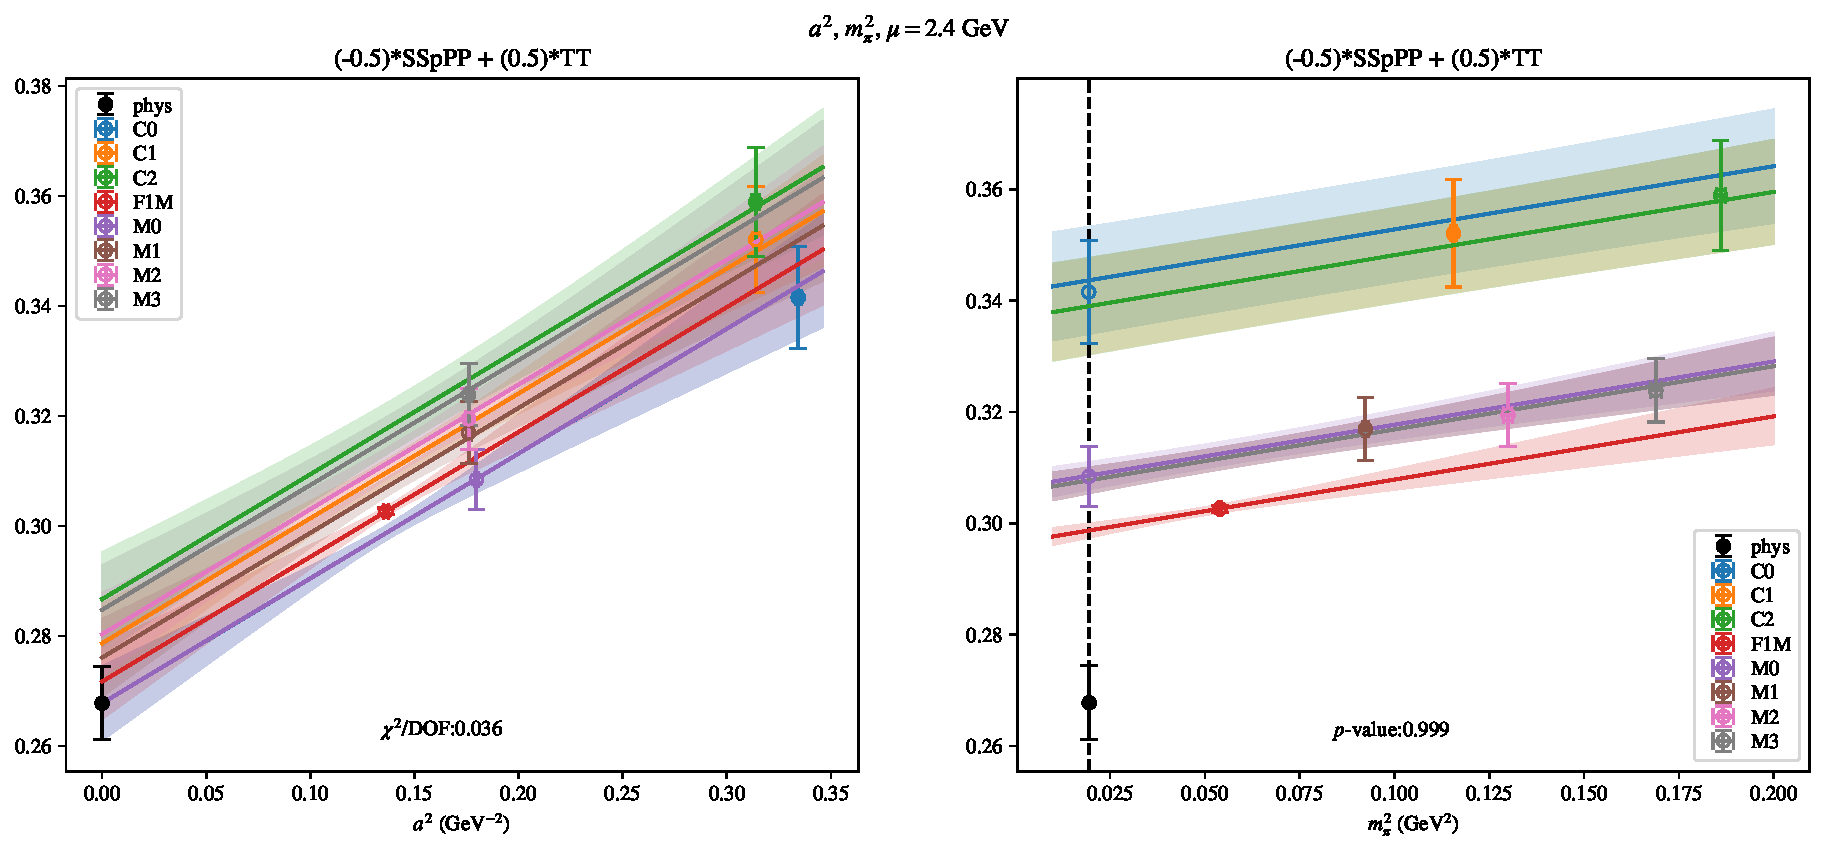
\includepdf[link, pages=-]{SSmPP/SUSY/a2m2_24.pdf}
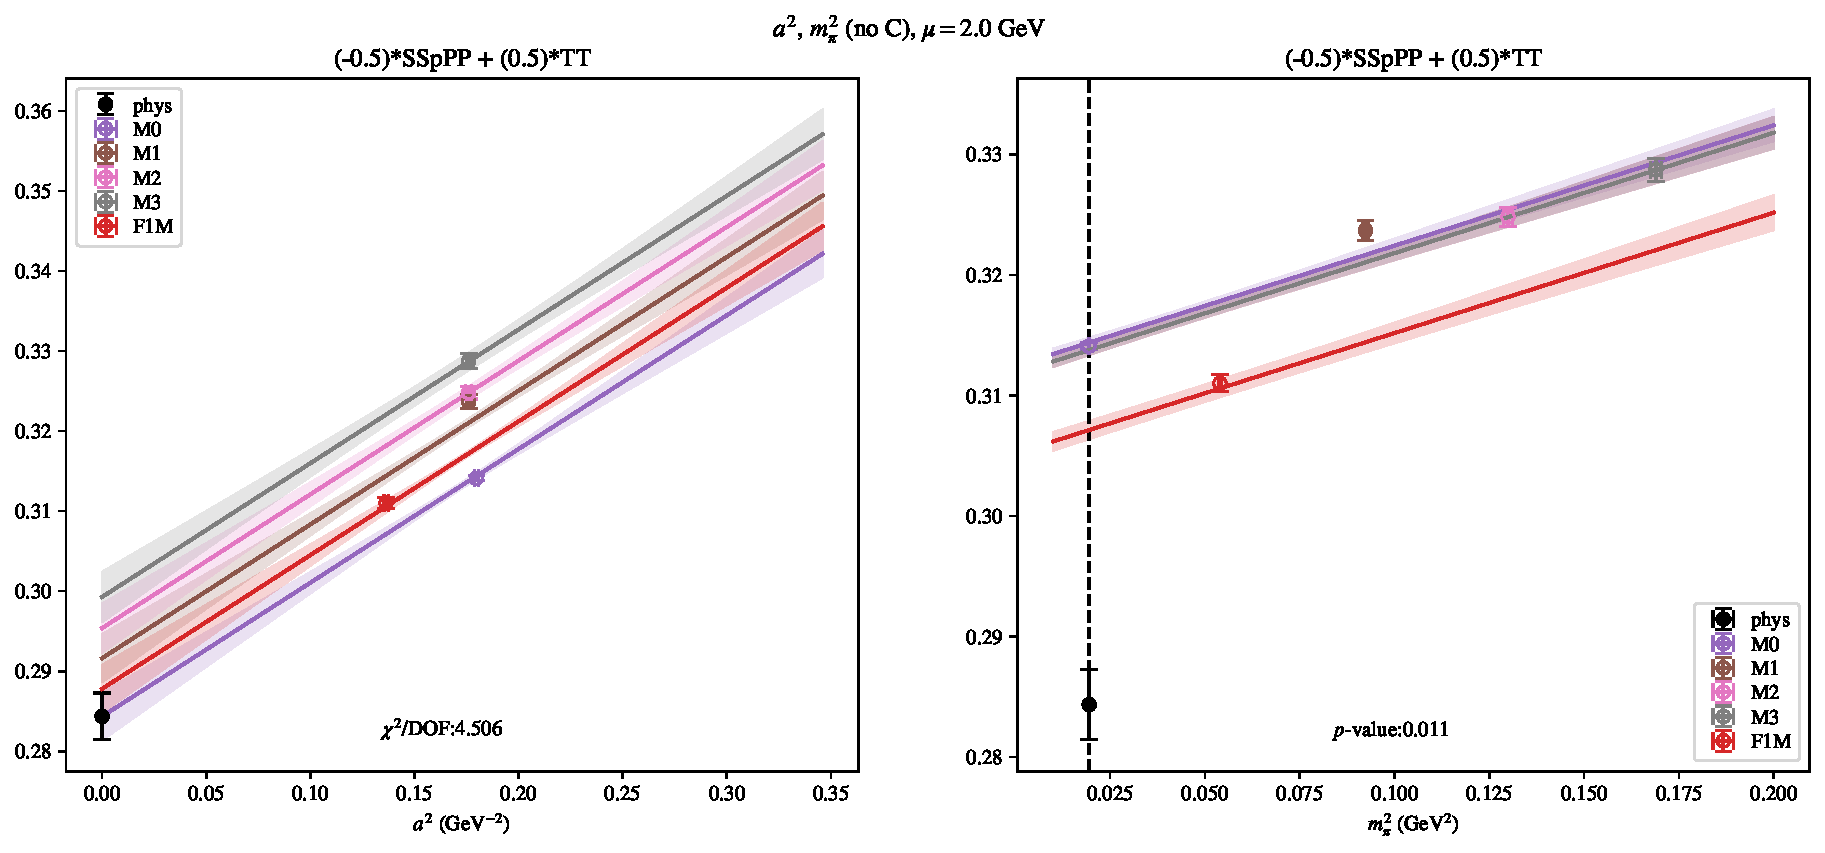
\includepdf[link, pages=-]{SSmPP/SUSY/a2m2noC_20.pdf}
\includepdf[link, pages=-]{SSmPP/SUSY/a2m2noC_22.pdf}
\includepdf[link, pages=-]{SSmPP/SUSY/a2m2noC_23.pdf}
\includepdf[link, pages=-]{SSmPP/SUSY/a2m2noC_24.pdf}
\includepdf[link, pages=-]{SSmPP/SUSY/a2a4m2_20.pdf}
\includepdf[link, pages=-]{SSmPP/SUSY/a2a4m2_22.pdf}
\includepdf[link, pages=-]{SSmPP/SUSY/a2a4m2_23.pdf}
\includepdf[link, pages=-]{SSmPP/SUSY/a2a4m2_24.pdf}
\includepdf[link, pages=-]{SSmPP/SUSY/a2m2mcut_20.pdf}
\includepdf[link, pages=-]{SSmPP/SUSY/a2m2mcut_22.pdf}
\includepdf[link, pages=-]{SSmPP/SUSY/a2m2mcut_23.pdf}
\includepdf[link, pages=-]{SSmPP/SUSY/a2m2mcut_24.pdf}
\includepdf[link, pages=-]{SSmPP/SUSY/a2m2m4_20.pdf}
\includepdf[link, pages=-]{SSmPP/SUSY/a2m2m4_22.pdf}
\includepdf[link, pages=-]{SSmPP/SUSY/a2m2m4_23.pdf}
\includepdf[link, pages=-]{SSmPP/SUSY/a2m2m4_24.pdf}
\clearpage
\section{$\mathcal{B}_4$}
\begin{table}[h!]
\begin{center}
\begin{tabular}{|c|c|c|c|c|c|}
\hline
$\mu$ (GeV) & $a^2$, $m_\pi^2$& $a^2$, $m_\pi^2$ (no C)& $a^2$, $a^4$, $m_\pi^2$& $a^2$, $m_\pi^2$ (no M3, C2)& $a^2$, $m_\pi^2$, $m_\pi^4$\\
\hline
2.0& \hyperlink{SSpPP/SUSY/a2m2_20.pdf.1}{\textbf{1.7999(28)}: 15.792 (0.0)} & \hyperlink{SSpPP/SUSY/a2m2noC_20.pdf.1}{\textbf{1.692(13)}: 0.632 (0.532)} & \hyperlink{SSpPP/SUSY/a2a4m2_20.pdf.1}{\textbf{1.622(20)}: 1.004 (0.404)} & \hyperlink{SSpPP/SUSY/a2m2mcut_20.pdf.1}{\textbf{1.8011(29)}: 24.886 (0.0)} & \hyperlink{SSpPP/SUSY/a2m2m4_20.pdf.1}{\textbf{1.8050(29)}: 15.279 (0.0)}\\
2.2& \hyperlink{SSpPP/SUSY/a2m2_22.pdf.1}{\textbf{1.8055(26)}: 14.677 (0.0)} & \hyperlink{SSpPP/SUSY/a2m2noC_22.pdf.1}{\textbf{1.705(12)}: 1.335 (0.263)} & \hyperlink{SSpPP/SUSY/a2a4m2_22.pdf.1}{\textbf{1.639(20)}: 1.485 (0.204)} & \hyperlink{SSpPP/SUSY/a2m2mcut_22.pdf.1}{\textbf{1.8069(28)}: 22.054 (0.0)} & \hyperlink{SSpPP/SUSY/a2m2m4_22.pdf.1}{\textbf{1.8106(28)}: 13.331 (0.0)}\\
2.3& \hyperlink{SSpPP/SUSY/a2m2_23.pdf.1}{\textbf{1.8079(26)}: 14.105 (0.0)} & \hyperlink{SSpPP/SUSY/a2m2noC_23.pdf.1}{\textbf{1.709(12)}: 1.491 (0.225)} & \hyperlink{SSpPP/SUSY/a2a4m2_23.pdf.1}{\textbf{1.645(20)}: 1.383 (0.237)} & \hyperlink{SSpPP/SUSY/a2m2mcut_23.pdf.1}{\textbf{1.8092(28)}: 21.411 (0.0)} & \hyperlink{SSpPP/SUSY/a2m2m4_23.pdf.1}{\textbf{1.8129(28)}: 13.139 (0.0)}\\
2.4& \hyperlink{SSpPP/SUSY/a2m2_24.pdf.1}{\textbf{1.8093(26)}: 13.073 (0.0)} & \hyperlink{SSpPP/SUSY/a2m2noC_24.pdf.1}{\textbf{1.714(12)}: 1.493 (0.225)} & \hyperlink{SSpPP/SUSY/a2a4m2_24.pdf.1}{\textbf{1.652(20)}: 1.366 (0.243)} & \hyperlink{SSpPP/SUSY/a2m2mcut_24.pdf.1}{\textbf{1.8105(28)}: 19.975 (0.0)} & \hyperlink{SSpPP/SUSY/a2m2m4_24.pdf.1}{\textbf{1.8141(28)}: 12.382 (0.0)}\\
\hline
\end{tabular}
\caption{Physical point value from chiral and continuum extrapolation at renormalisation scale $\mu$. Entries are \textbf{value(error)}: $\chi^2/\text{DOF}$ ($p$-value).}
\end{center}
\end{table}
\begin{table}[h!]
\begin{center}
\begin{tabular}{|c c|c|c|c|c|c|}
\hline
$\mu$ (GeV) &  & $a^2$, $m_\pi^2$& $a^2$, $m_\pi^2$ (no C)& $a^2$, $a^4$, $m_\pi^2$& $a^2$, $m_\pi^2$ (no M3, C2)& $a^2$, $m_\pi^2$, $m_\pi^4$\\
\hline
\multirow{2}{0.5in}{2.0} & $\alpha$ & 0.0708(59)& 0.446(47)& 1.06(12)& 0.0687(61)& 0.0614(62)\\
 & $\beta$ & -0.0010(13)& -0.0011(26)& -0.0015(15)& -0.0015(24)& -0.0040(69)\\
\hline
\multirow{2}{0.5in}{2.2} & $\alpha$ & 0.0763(57)& 0.425(46)& 0.99(12)& 0.0742(60)& 0.0670(59)\\
 & $\beta$ & -0.0007(12)& -0.0008(24)& -0.0011(14)& -0.0012(23)& -0.0037(65)\\
\hline
\multirow{2}{0.5in}{2.3} & $\alpha$ & 0.0774(56)& 0.417(45)& 0.97(12)& 0.0754(59)& 0.0683(59)\\
 & $\beta$ & -0.0006(12)& -0.0008(22)& -0.0011(14)& -0.0011(22)& -0.0034(64)\\
\hline
\multirow{2}{0.5in}{2.4} & $\alpha$ & 0.0792(55)& 0.406(45)& 0.93(12)& 0.0774(59)& 0.0704(59)\\
 & $\beta$ & -0.0006(11)& -0.0007(21)& -0.0010(13)& -0.0010(22)& -0.0031(62)\\
\hline
\end{tabular}
\caption{Fit values of coefficients in $Q = Q_{phys} + \mathbf{\alpha} a^2 + \mathbf{\beta}\left(\frac{m_\pi^2}{f_\pi^2}-\frac{m_{\pi,PDG}^2}{f_\pi^2}\right) + \ldots$.}
\end{center}
\end{table}
\includepdf[link, pages=-]{SSpPP/SUSY/a2m2_20.pdf}
\includepdf[link, pages=-]{SSpPP/SUSY/a2m2_22.pdf}
\includepdf[link, pages=-]{SSpPP/SUSY/a2m2_23.pdf}
\includepdf[link, pages=-]{SSpPP/SUSY/a2m2_24.pdf}
\includepdf[link, pages=-]{SSpPP/SUSY/a2m2noC_20.pdf}
\includepdf[link, pages=-]{SSpPP/SUSY/a2m2noC_22.pdf}
\includepdf[link, pages=-]{SSpPP/SUSY/a2m2noC_23.pdf}
\includepdf[link, pages=-]{SSpPP/SUSY/a2m2noC_24.pdf}
\includepdf[link, pages=-]{SSpPP/SUSY/a2a4m2_20.pdf}
\includepdf[link, pages=-]{SSpPP/SUSY/a2a4m2_22.pdf}
\includepdf[link, pages=-]{SSpPP/SUSY/a2a4m2_23.pdf}
\includepdf[link, pages=-]{SSpPP/SUSY/a2a4m2_24.pdf}
\includepdf[link, pages=-]{SSpPP/SUSY/a2m2mcut_20.pdf}
\includepdf[link, pages=-]{SSpPP/SUSY/a2m2mcut_22.pdf}
\includepdf[link, pages=-]{SSpPP/SUSY/a2m2mcut_23.pdf}
\includepdf[link, pages=-]{SSpPP/SUSY/a2m2mcut_24.pdf}
\includepdf[link, pages=-]{SSpPP/SUSY/a2m2m4_20.pdf}
\includepdf[link, pages=-]{SSpPP/SUSY/a2m2m4_22.pdf}
\includepdf[link, pages=-]{SSpPP/SUSY/a2m2m4_23.pdf}
\includepdf[link, pages=-]{SSpPP/SUSY/a2m2m4_24.pdf}
\clearpage
\section{$\mathcal{B}_5$}
\begin{table}[h!]
\begin{center}
\begin{tabular}{|c|c|c|c|c|c|}
\hline
$\mu$ (GeV) & $a^2$, $m_\pi^2$& $a^2$, $m_\pi^2$ (no C)& $a^2$, $a^4$, $m_\pi^2$& $a^2$, $m_\pi^2$ (no M3, C2)& $a^2$, $m_\pi^2$, $m_\pi^4$\\
\hline
2.0& \hyperlink{TT/SUSY/a2m2_20.pdf.1}{\textbf{0.49582(79)}: 10.301 (0.0)} & \hyperlink{TT/SUSY/a2m2noC_20.pdf.1}{\textbf{0.4656(44)}: 1.83 (0.16)} & \hyperlink{TT/SUSY/a2a4m2_20.pdf.1}{\textbf{0.4491(68)}: 1.817 (0.122)} & \hyperlink{TT/SUSY/a2m2mcut_20.pdf.1}{\textbf{0.49608(79)}: 16.122 (0.0)} & \hyperlink{TT/SUSY/a2m2m4_20.pdf.1}{\textbf{0.49675(81)}: 9.907 (0.0)}\\
2.2& \hyperlink{TT/SUSY/a2m2_22.pdf.1}{\textbf{0.50288(74)}: 10.029 (0.0)} & \hyperlink{TT/SUSY/a2m2noC_22.pdf.1}{\textbf{0.4750(44)}: 2.919 (0.054)} & \hyperlink{TT/SUSY/a2a4m2_22.pdf.1}{\textbf{0.4601(69)}: 2.575 (0.036)} & \hyperlink{TT/SUSY/a2m2mcut_22.pdf.1}{\textbf{0.50319(75)}: 14.189 (0.0)} & \hyperlink{TT/SUSY/a2m2m4_22.pdf.1}{\textbf{0.50389(76)}: 8.538 (0.0)}\\
2.3& \hyperlink{TT/SUSY/a2m2_23.pdf.1}{\textbf{0.50603(73)}: 10.128 (0.0)} & \hyperlink{TT/SUSY/a2m2noC_23.pdf.1}{\textbf{0.4784(43)}: 3.114 (0.044)} & \hyperlink{TT/SUSY/a2a4m2_23.pdf.1}{\textbf{0.4633(68)}: 2.454 (0.044)} & \hyperlink{TT/SUSY/a2m2mcut_23.pdf.1}{\textbf{0.50631(74)}: 14.515 (0.0)} & \hyperlink{TT/SUSY/a2m2m4_23.pdf.1}{\textbf{0.50702(76)}: 8.927 (0.0)}\\
2.4& \hyperlink{TT/SUSY/a2m2_24.pdf.1}{\textbf{0.50838(72)}: 9.305 (0.0)} & \hyperlink{TT/SUSY/a2m2noC_24.pdf.1}{\textbf{0.4821(42)}: 3.086 (0.046)} & \hyperlink{TT/SUSY/a2a4m2_24.pdf.1}{\textbf{0.4688(68)}: 2.623 (0.033)} & \hyperlink{TT/SUSY/a2m2mcut_24.pdf.1}{\textbf{0.50859(75)}: 13.197 (0.0)} & \hyperlink{TT/SUSY/a2m2m4_24.pdf.1}{\textbf{0.50935(77)}: 8.289 (0.0)}\\
\hline
\end{tabular}
\caption{Physical point value from chiral and continuum extrapolation at renormalisation scale $\mu$. Entries are \textbf{value(error)}: $\chi^2/\text{DOF}$ ($p$-value).}
\end{center}
\end{table}
\begin{table}[h!]
\begin{center}
\begin{tabular}{|c c|c|c|c|c|c|}
\hline
$\mu$ (GeV) &  & $a^2$, $m_\pi^2$& $a^2$, $m_\pi^2$ (no C)& $a^2$, $a^4$, $m_\pi^2$& $a^2$, $m_\pi^2$ (no M3, C2)& $a^2$, $m_\pi^2$, $m_\pi^4$\\
\hline
\multirow{2}{0.5in}{2.0} & $\alpha$ & -0.183(55)& 0.176(56)& 0.71(14)& -0.184(55)& -0.189(57)\\
 & $\beta$ & 0.00106(14)& 0.00114(26)& 0.00085(17)& 0.00071(24)& -0.0014(73)\\
\hline
\multirow{2}{0.5in}{2.2} & $\alpha$ & -0.223(52)& 0.099(53)& 0.57(14)& -0.225(52)& -0.229(53)\\
 & $\beta$ & 0.00116(13)& 0.00120(23)& 0.00098(15)& 0.00067(22)& -0.0014(66)\\
\hline
\multirow{2}{0.5in}{2.3} & $\alpha$ & -0.246(52)& 0.070(52)& 0.54(14)& -0.247(53)& -0.251(53)\\
 & $\beta$ & 0.00116(13)& 0.00119(22)& 0.00098(15)& 0.00070(22)& -0.0012(65)\\
\hline
\multirow{2}{0.5in}{2.4} & $\alpha$ & -0.265(52)& 0.031(50)& 0.45(13)& -0.266(53)& -0.271(54)\\
 & $\beta$ & 0.00112(12)& 0.00120(21)& 0.00095(15)& 0.00070(21)& -0.0011(64)\\
\hline
\end{tabular}
\caption{Fit values of coefficients in $Q = Q_{phys} + \mathbf{\alpha} a^2 + \mathbf{\beta}\left(\frac{m_\pi^2}{f_\pi^2}-\frac{m_{\pi,PDG}^2}{f_\pi^2}\right) + \ldots$.}
\end{center}
\end{table}
\includepdf[link, pages=-]{TT/SUSY/a2m2_20.pdf}
\includepdf[link, pages=-]{TT/SUSY/a2m2_22.pdf}
\includepdf[link, pages=-]{TT/SUSY/a2m2_23.pdf}
\includepdf[link, pages=-]{TT/SUSY/a2m2_24.pdf}
\includepdf[link, pages=-]{TT/SUSY/a2m2noC_20.pdf}
\includepdf[link, pages=-]{TT/SUSY/a2m2noC_22.pdf}
\includepdf[link, pages=-]{TT/SUSY/a2m2noC_23.pdf}
\includepdf[link, pages=-]{TT/SUSY/a2m2noC_24.pdf}
\includepdf[link, pages=-]{TT/SUSY/a2a4m2_20.pdf}
\includepdf[link, pages=-]{TT/SUSY/a2a4m2_22.pdf}
\includepdf[link, pages=-]{TT/SUSY/a2a4m2_23.pdf}
\includepdf[link, pages=-]{TT/SUSY/a2a4m2_24.pdf}
\includepdf[link, pages=-]{TT/SUSY/a2m2mcut_20.pdf}
\includepdf[link, pages=-]{TT/SUSY/a2m2mcut_22.pdf}
\includepdf[link, pages=-]{TT/SUSY/a2m2mcut_23.pdf}
\includepdf[link, pages=-]{TT/SUSY/a2m2mcut_24.pdf}
\includepdf[link, pages=-]{TT/SUSY/a2m2m4_20.pdf}
\includepdf[link, pages=-]{TT/SUSY/a2m2m4_22.pdf}
\includepdf[link, pages=-]{TT/SUSY/a2m2m4_23.pdf}
\includepdf[link, pages=-]{TT/SUSY/a2m2m4_24.pdf}
\clearpage
\end{document}